% ════════════════════════════════════════════
% 结果分析（05.模型建立求解.tex，一级章节包装）
% ════════════════════════════════════════════
\section{结果分析}

本章按数据诊断、数据整理、回归建模与效应测算四个环节呈现结果。每一节先说明该环节要回答的问题与采用的口径，再给出关键图表与数值，最后归纳对后续环节的含义。四节使用同一份 500 条帖子的分析数据，图表编号连续，全部数值由求解目录中的主程序生成。


% ════════════════════════════════════════════
% 数据理解与分布诊断（5.1）
% ════════════════════════════════════════════
\subsection{数据理解与分布诊断}

\subsubsection{数据口径与变量角色}

本部分不追求拟合模型，而是要把“数据能支持什么样的模型”说清楚。原始表共 500 行、8 个字段，一行即一条帖子，7 个输入变量加 1 个曝光结果；没有帖子编号与发布时间戳，同一主页只有一次观测，因此判定为帖子级截面数据，而不是面板或时间序列。按发帖前运营人员能否决定，帖子类型、内容主题、月份、星期、时段与付费标记属于发帖决策变量；粉丝规模由历史积累决定，属于账号状态变量；曝光总次数是发布后的结果。图\ref{fig:q1_dict}把变量的类型、取值类别与缺失状态集中呈现：X1 为连续变量但有 90 个重复取值，X2、X3 为名义变量，X4 至 X6 为周期性时间标记，X7 为二元指示变量且是唯一存在缺失的字段，Y1 为连续计数结果。计量单位上，X1 以人、Y1 以次计，X4、X5、X6 分别以月、星期与小时计；这些口径在后续所有模型中保持不变。

\begin{figure}[ht]
  \centering
  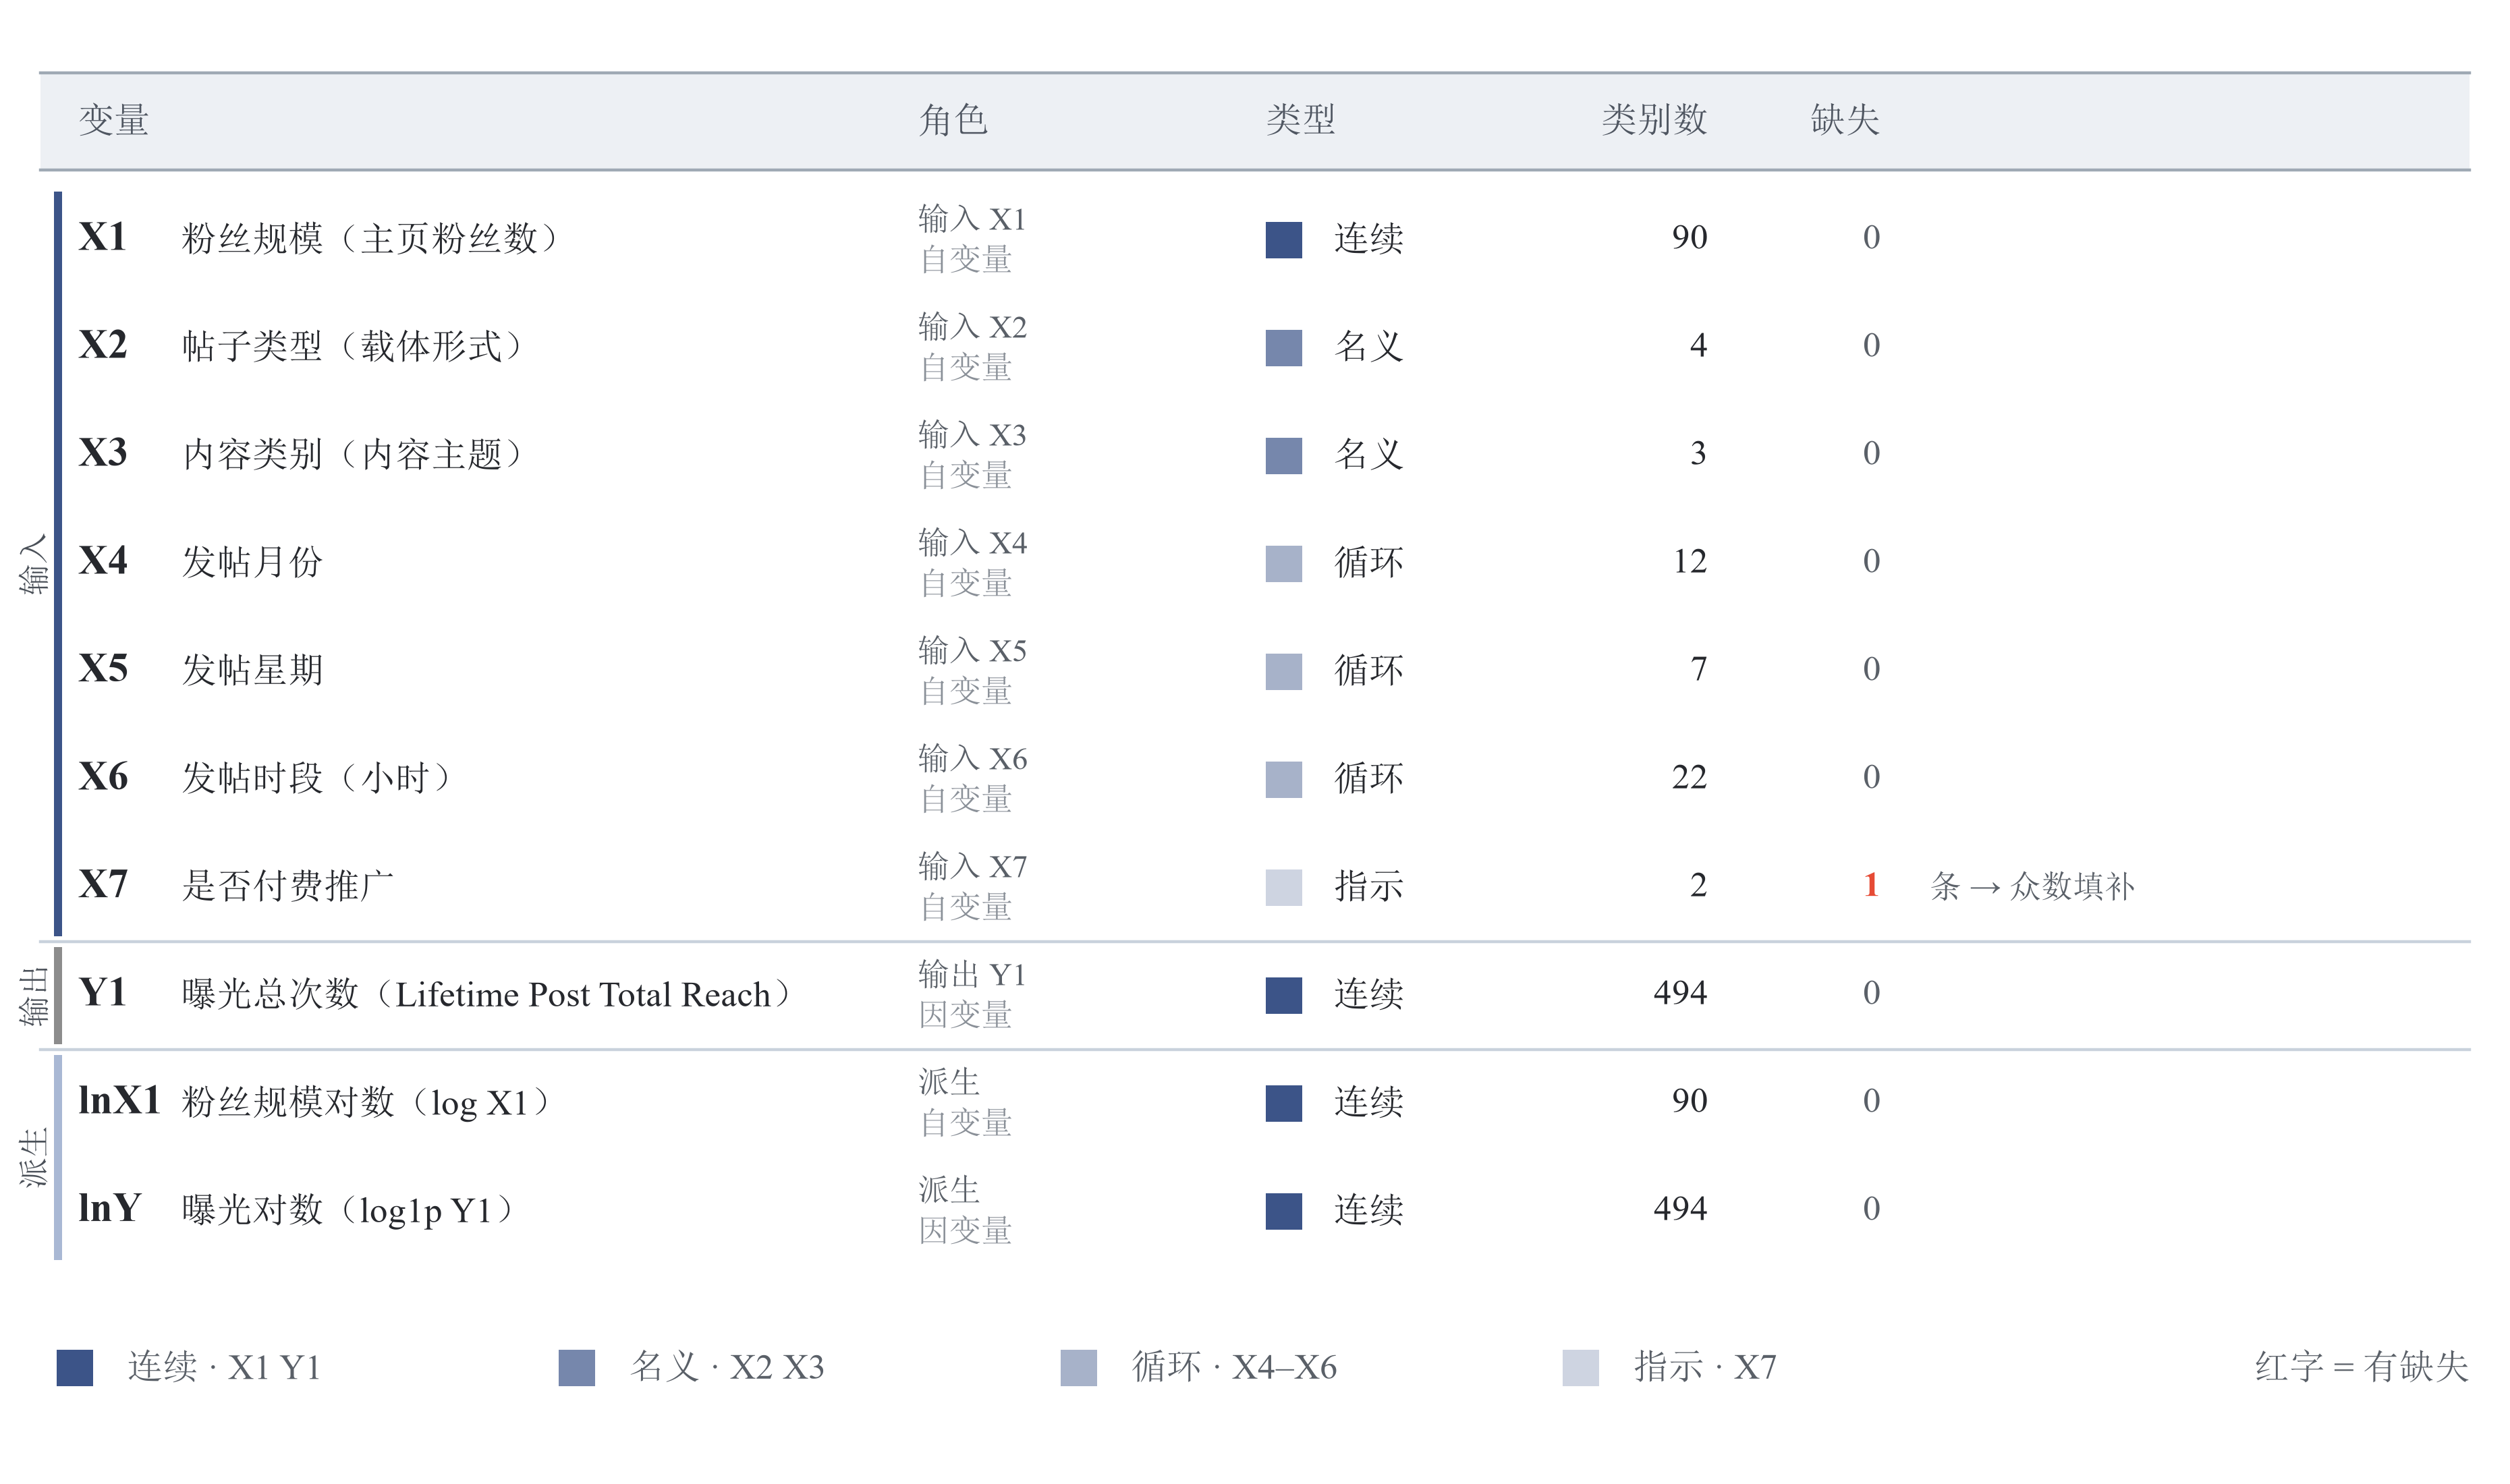
\includegraphics[width=0.68\textwidth]{../求解/问题一/结果/图14_变量字典与缺失.png}
  \caption{变量字典、类型与缺失状态}
  \label{fig:q1_dict}
\end{figure}

图\ref{fig:q1_dict}还显示，X1 只有 90 个不同取值，说明粉丝数按天或按批次更新，同一数值被多条帖子共享；X6 在样本中有 22 个取值，0 时与 21 时没有帖子；Y1 有 494 个不同取值，只有少数重复。上述结构决定了后续不能把 X1 当作独立的时间序列，也不能对 X6 逐小时生成哑变量。

\subsubsection{分布形态与共线证据}

曝光量呈典型的重尾右偏。表\ref{tab:q1_desc}显示，均值为 29,586 次，约为中位数 9,051 次的 3.27 倍；最大值 1,110,282 次为中位数的 122.67 倍；偏度 8.33、峰度 93.05，远超正态分布的参考范围。粉丝规模均值 123,194 人、标准差 16,273 人，最大值与最小值之比仅 1.71，量级跨度有限。付费帖子 139 条，占 499 条有效记录的 27.9\%，填补后占 500 条的 27.8\%。

图\ref{fig:q1_dist}把分布与分组差异放在同一画布。左上直方图在对数横轴上仍向右拖尾，中位数附近堆积了大量帖子，10 万次以上的极端帖子数量很少；右上雨云图显示，付费组的中位曝光为 12,060 次、自然组为 8,443 次（完整案例 $n=360$），中位数提升 42.8\%。下方按类型与主题分组的雨云图表明，视频组的中位数最高（56,950 次），状态组次之（20,849 次），图片组与链接组接近（8,132 与 9,773 次），三类主题的中位数分别为 10,417、8,962 与 8,303 次。分组差异为后续回归提供了初步线索，但未控制月份与内容构成，不能直接当作净效应。

\begin{figure}[p]
  \centering
  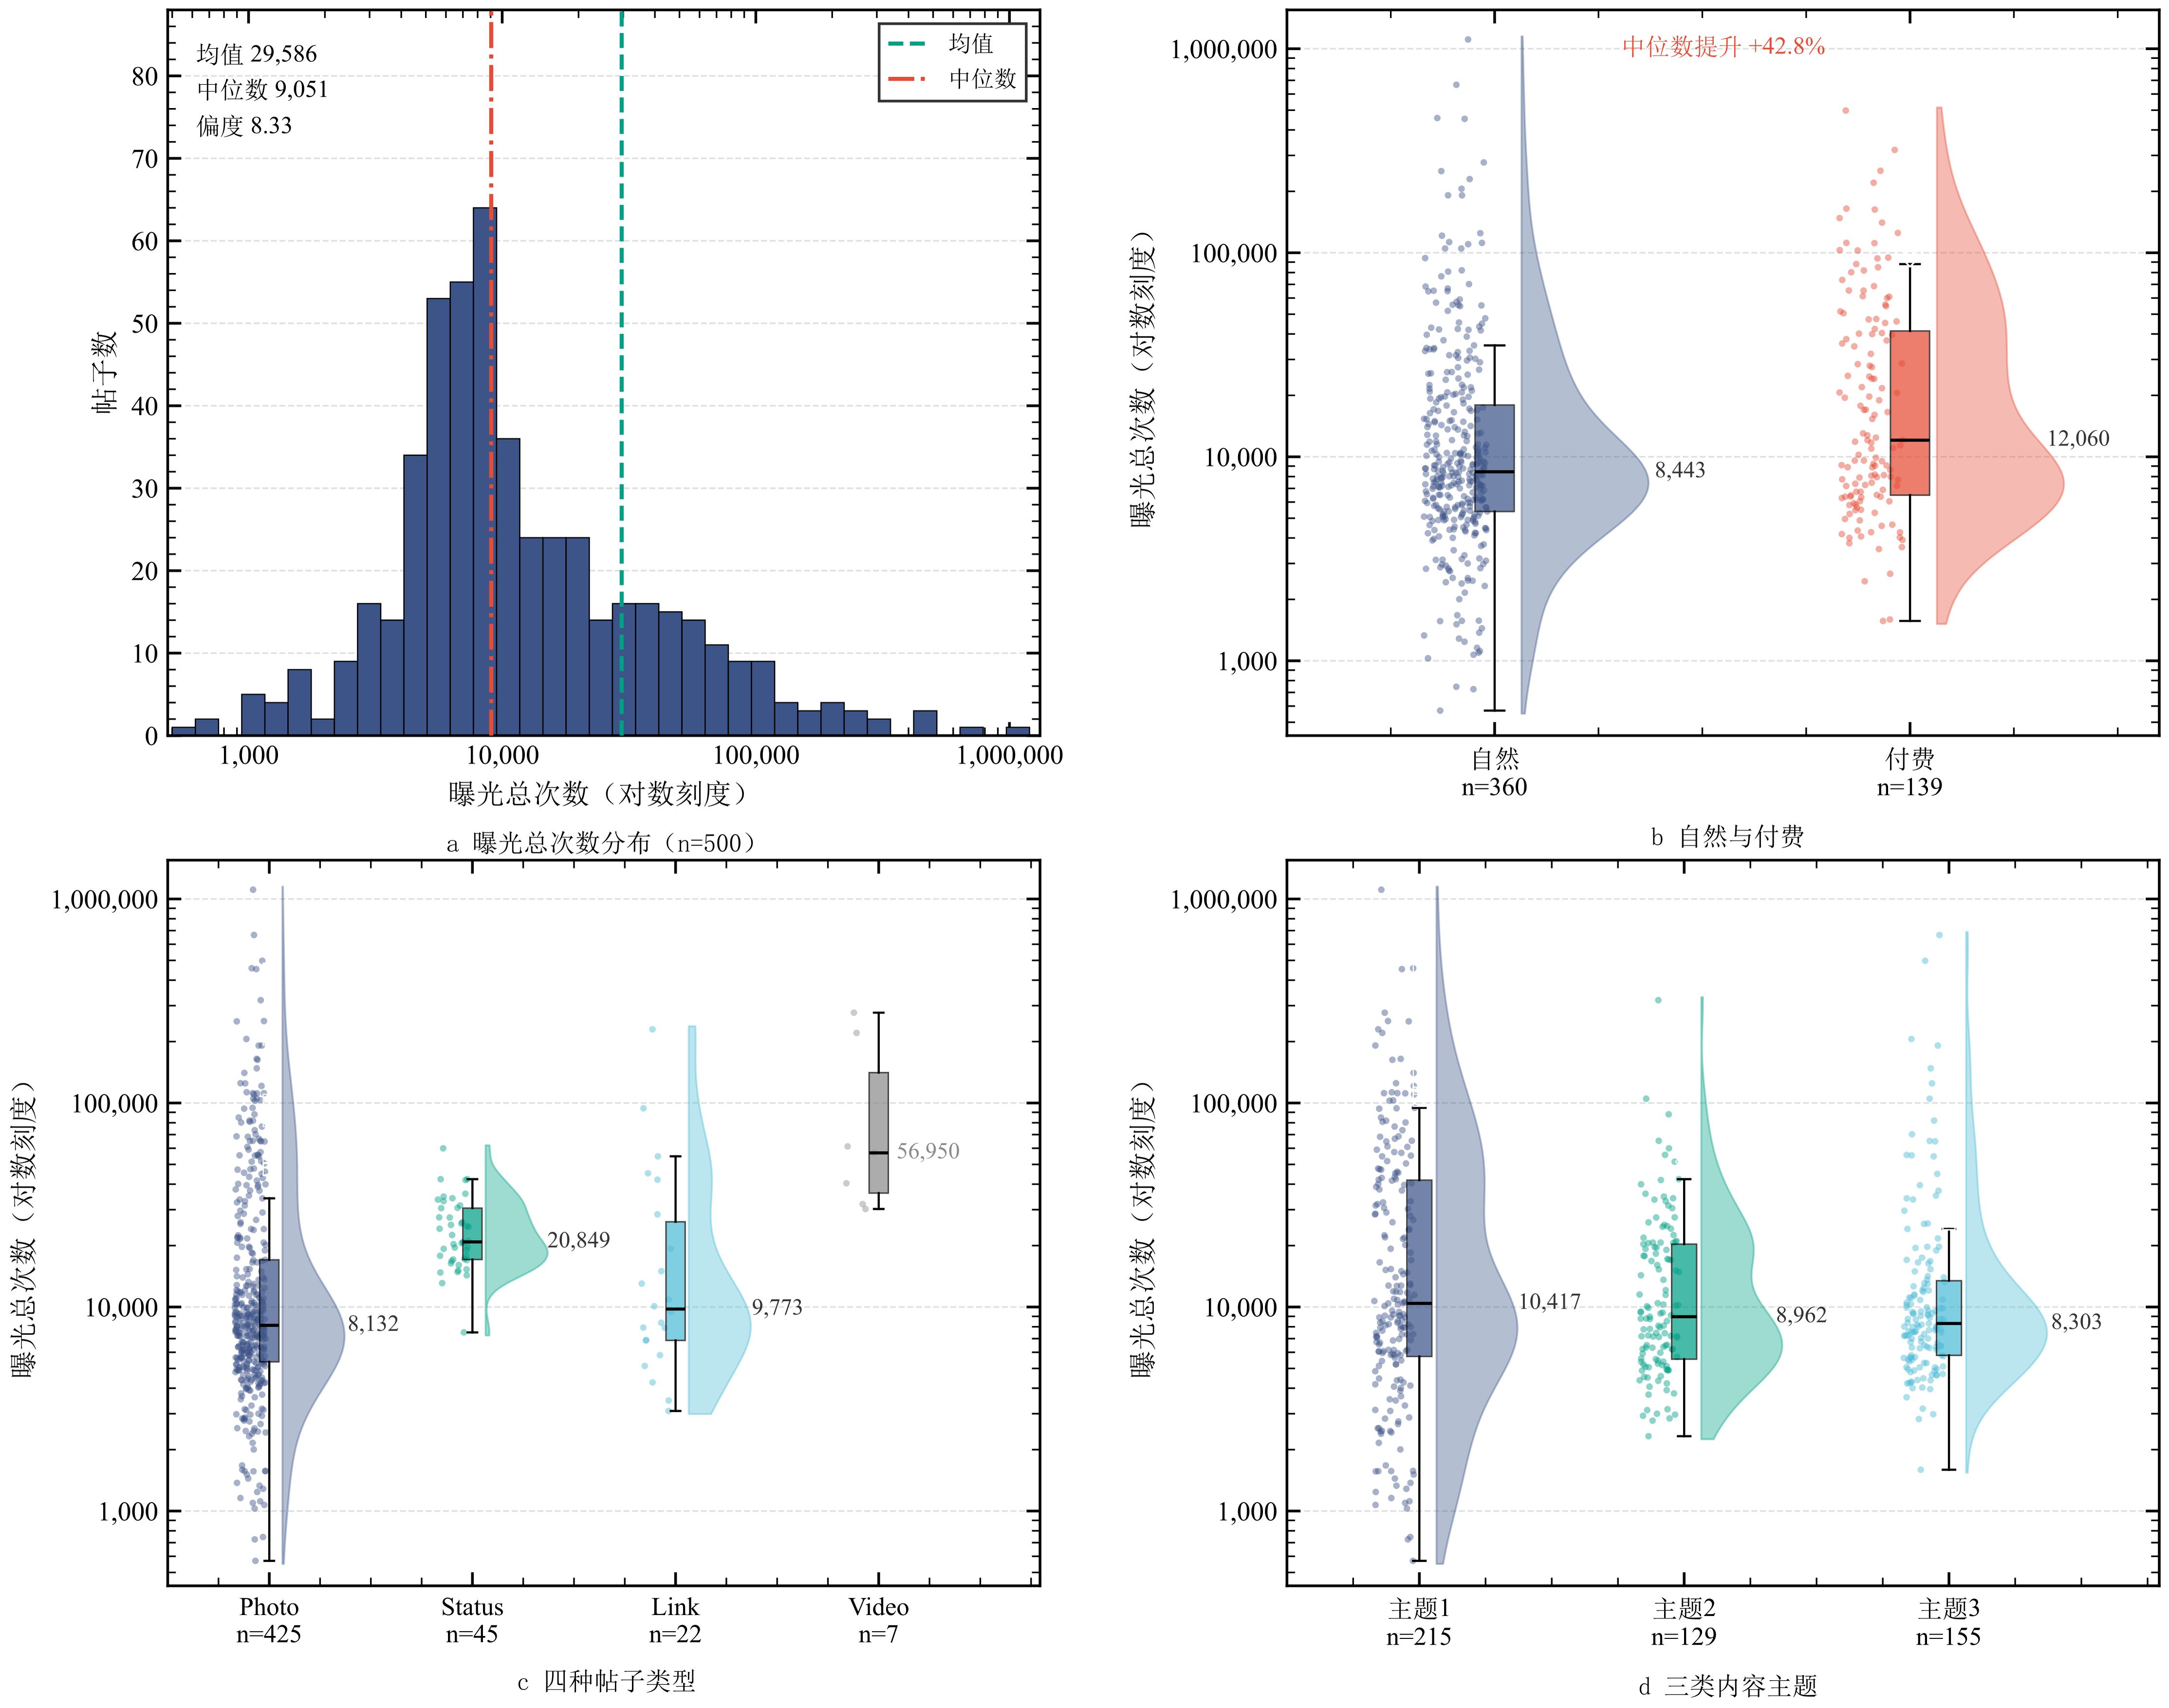
\includegraphics[width=0.66\textwidth]{../求解/问题一/结果/图1_曝光与分组分布.png}
  \caption{曝光量分布与分组差异}
  \label{fig:q1_dist}
\end{figure}

图\ref{fig:q1_structure}从构成、主题分布与联合分布三个角度补充样本结构。左上图以中线为界，左侧为自然帖、右侧为付费帖：Photo 在两组中都占 85\% 以上（自然 307 条、付费 119 条），Status 与 Link 合计不足 15\%，Video 只有 7 条且其中 4 条为付费，付费占比 57.1\%，说明类型效应主要由 Photo 与 Status 支撑，Video 的估计必然带有较大不确定性。右上图把三类主题的曝光分布、箱线与原始散点叠在一起，三组对数曝光的中位数分别为 9.25、9.09、9.02，主题 1 的分布整体略高，但三组重叠很大，单看主题不足以区分帖子表现。下方联合密度图的散点呈近竖直云团，粉丝规模对数与曝光对数的 Pearson 相关系数仅为 $-0.082$（$p=0.066$），上缘与右缘的边缘直方图进一步显示：两组在粉丝规模上几乎完全重合，而在曝光轴上付费组整体右移。由此可见，粉丝规模既不能单独解释曝光，也不足以区分付费与自然帖子，后续模型应把重点放在内容与投放变量上。

\begin{figure}[p]
  \centering
  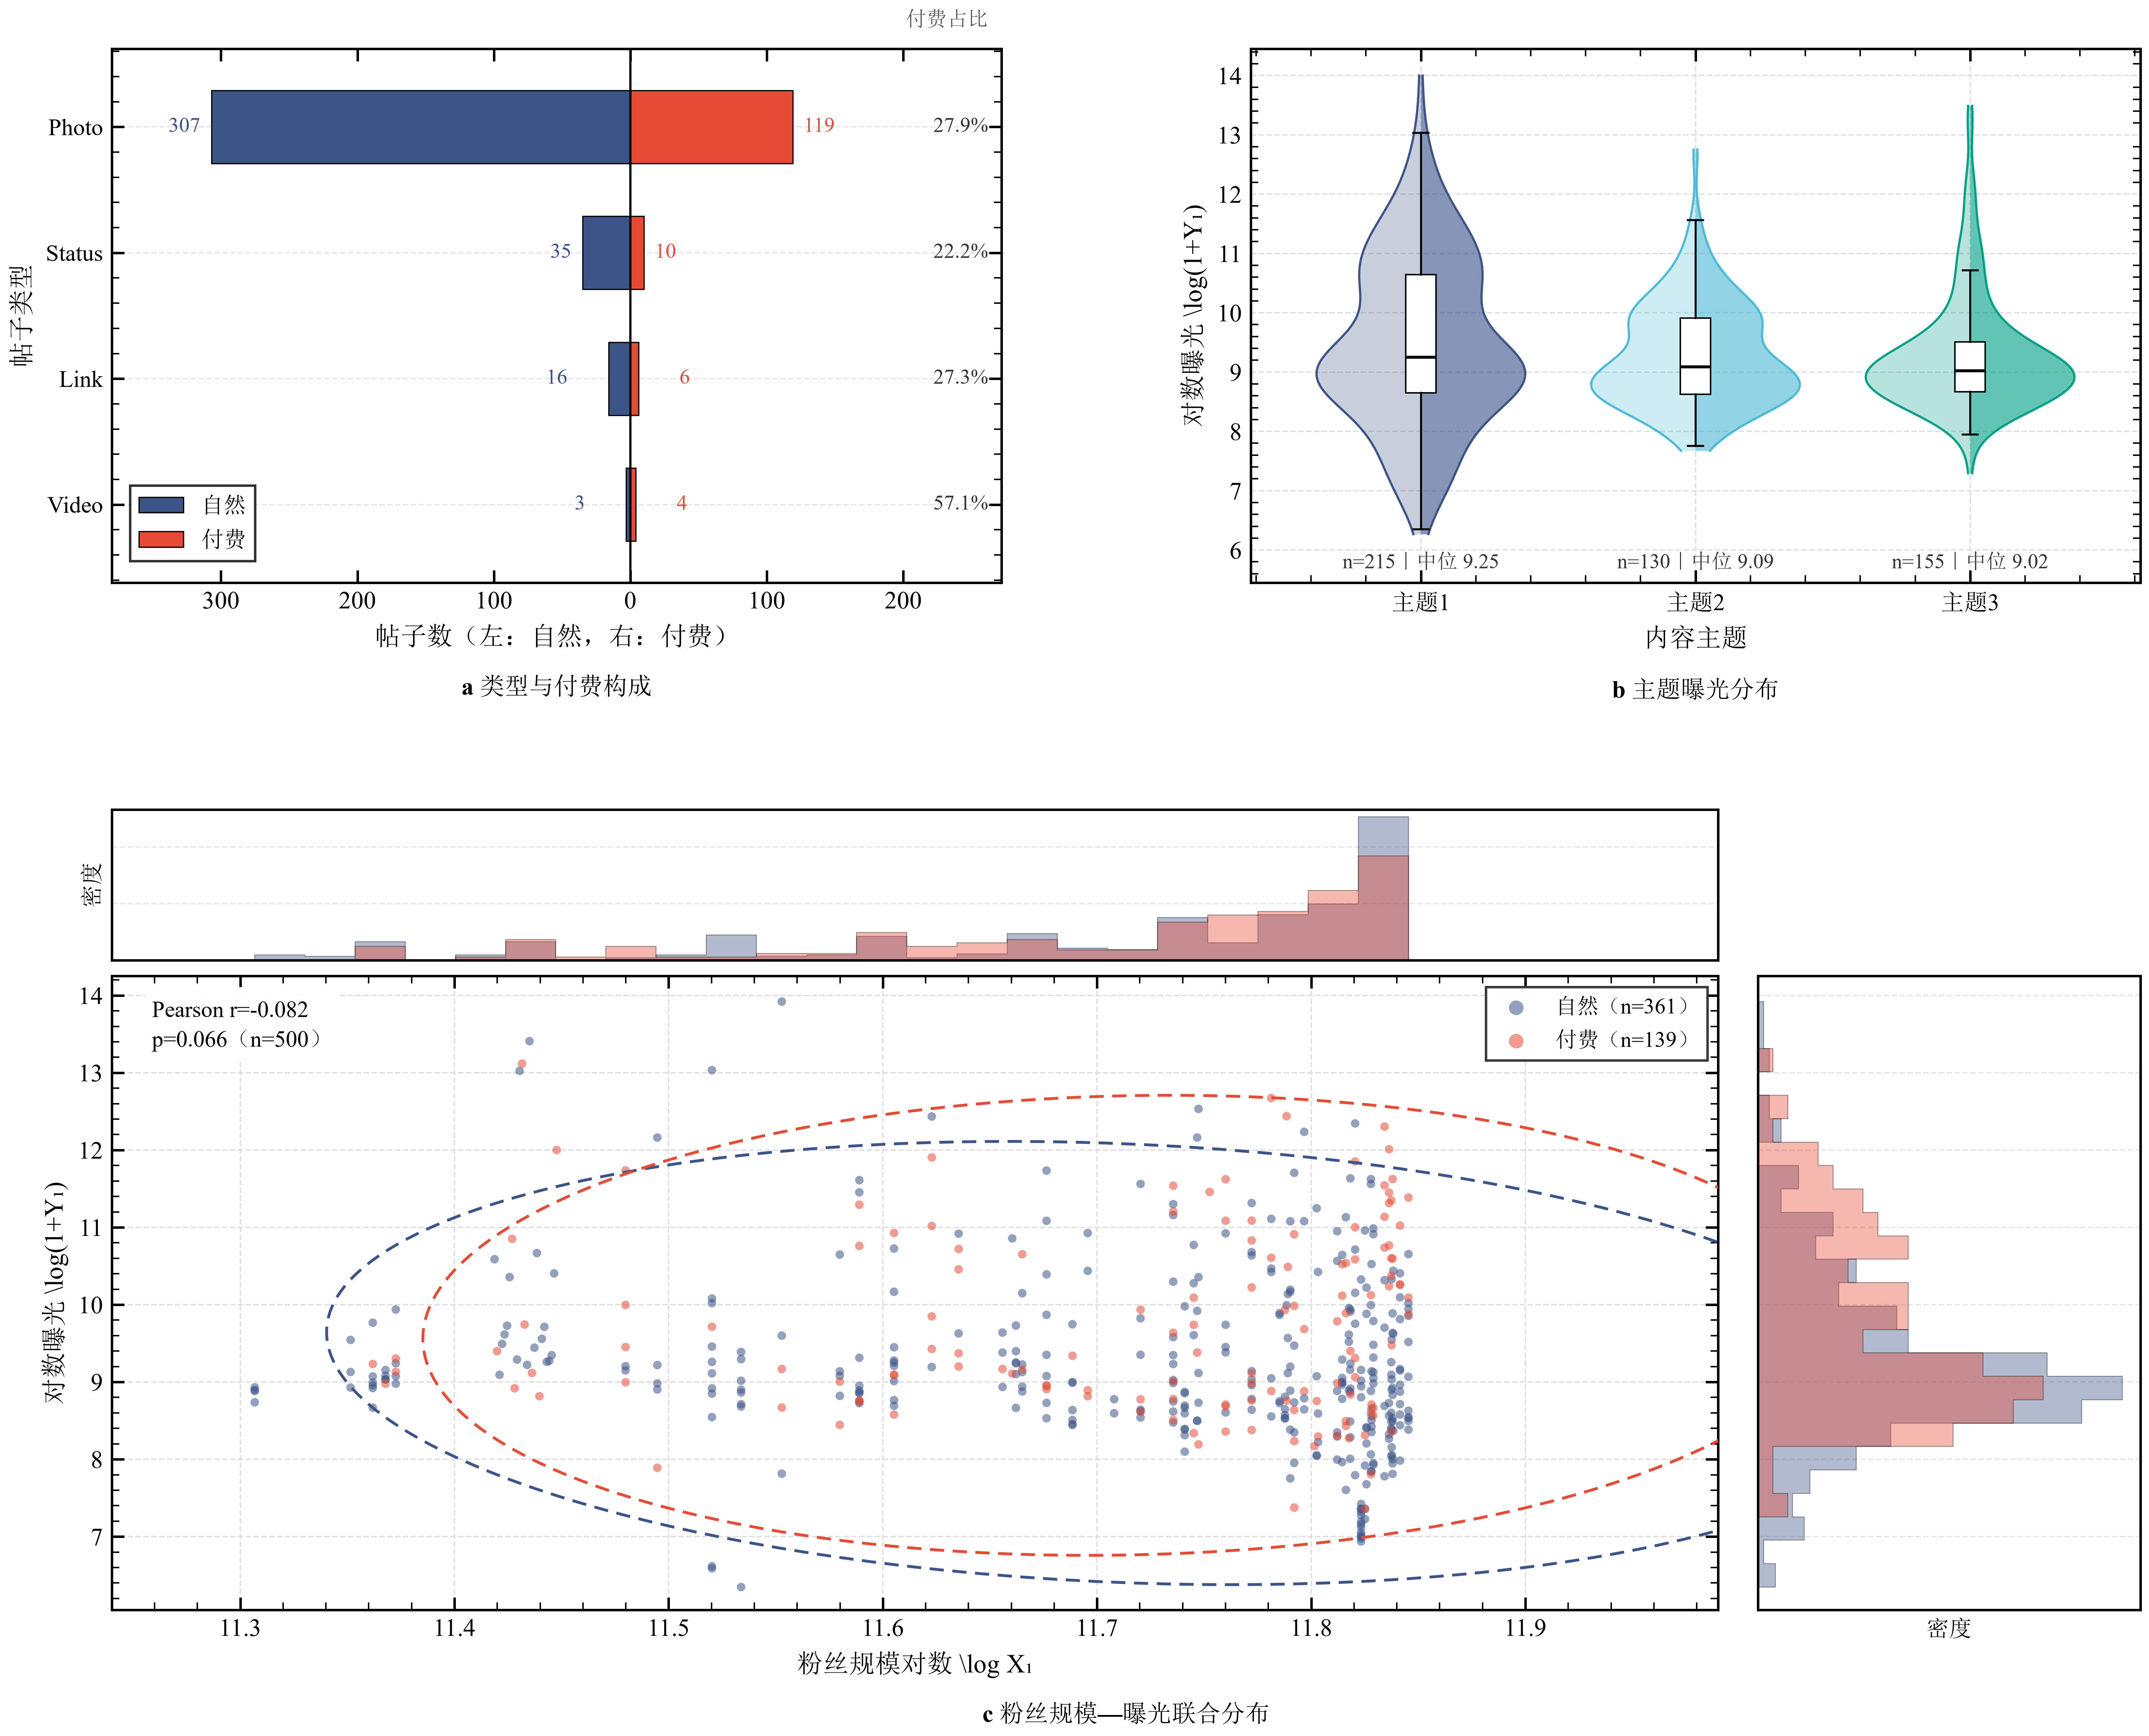
\includegraphics[width=0.66\textwidth]{../求解/临时产物/补充图1_样本结构.png}
  \caption{样本构成、主题分布与粉丝—曝光联合分布}
  \label{fig:q1_structure}
\end{figure}

表\ref{tab:q1_desc}同时给出共线证据。粉丝规模与月份的 Pearson 相关为 0.941、Spearman 相关为 0.996；以月份哑变量对粉丝规模对数做辅助回归，解释度达 0.9917，月内标准差仅 0.0130，月内方差占比仅 0.83\%。按预设的三项判别标准，粉丝规模与月份属于同一变异维度，同时进入回归会使系数依赖极少量月内变异。这一结构在散点与月均值折线上表现为阶梯式上升：月均值几乎单调递增，同一月份内部的粉丝规模对数只在极小范围内波动，偏差幅度远小于月间差异。这意味着粉丝规模在本样本中更接近“时间标签”而非独立解释变量。

\begin{figure}[htbp]
  \centering
  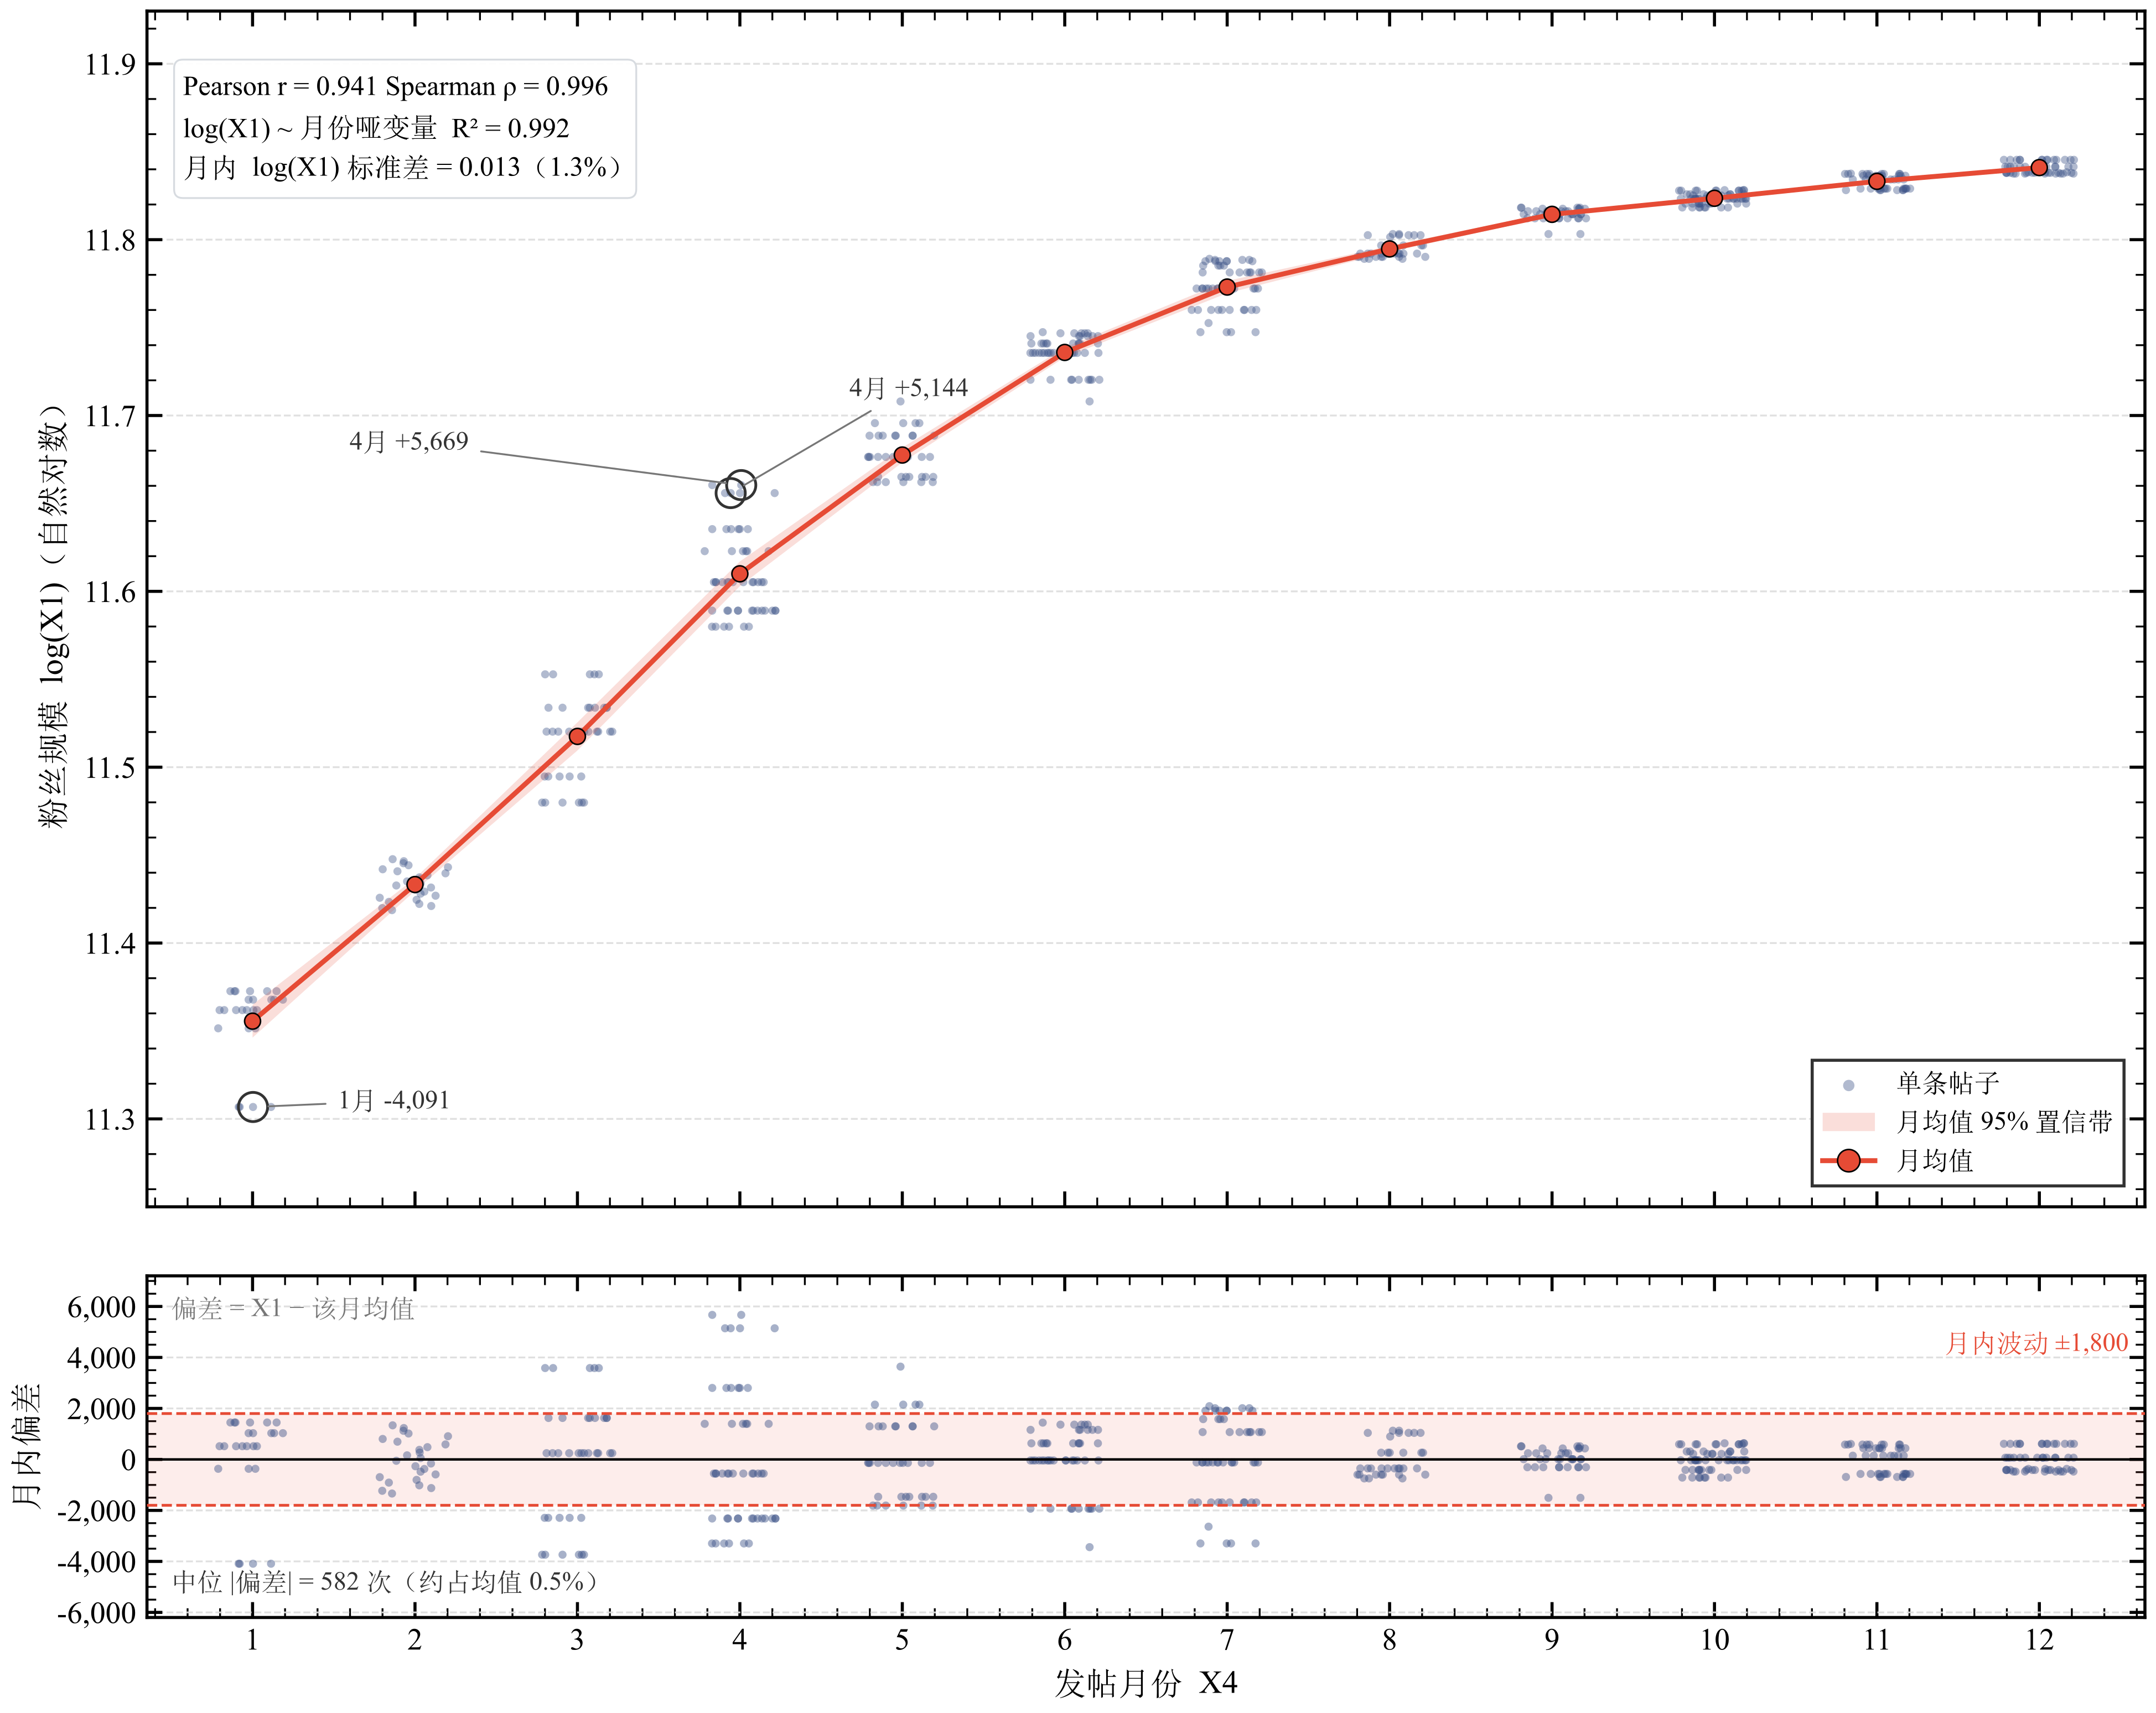
\includegraphics[width=0.74\textwidth]{../求解/问题一/结果/图2_粉丝规模与月份共线.png}
  \caption{粉丝规模与月份的共线结构：月度阶梯与月内偏差}
  \label{fig:q1_collinear}
\end{figure}

图\ref{fig:q1_collinear}把这一结构直接画了出来：主图按月排列的散点几乎落在同一条单调上升的曲线上，红色折线为月均值、浅红带为 95\% 置信带，圈注点为月内偏差最大的三条帖子；下挂小图给出每条帖子相对当月均值的偏差，绝大多数落在 $\pm 1{,}800$ 次以内，中位绝对偏差仅 582 次，与月间上万次的落差形成鲜明对比。

相关分析进一步给出主要变量的 Spearman 相关矩阵。曝光量与付费的相关系数为 0.171，是矩阵中与曝光关系最强的一项；与粉丝规模、月份的相关系数均为 $-0.135$，与内容主题为 $-0.080$，方向虽为负但幅度都很小；粉丝规模与月份的相关系数为 0.996，是矩阵中最突出的一格，说明二者几乎携带同一信息。相关矩阵只反映两两关系，且不包含帖子类型与发布时段，仍需回归控制其他变量后才能判断净效应。

\begin{figure}[htbp]
  \centering
  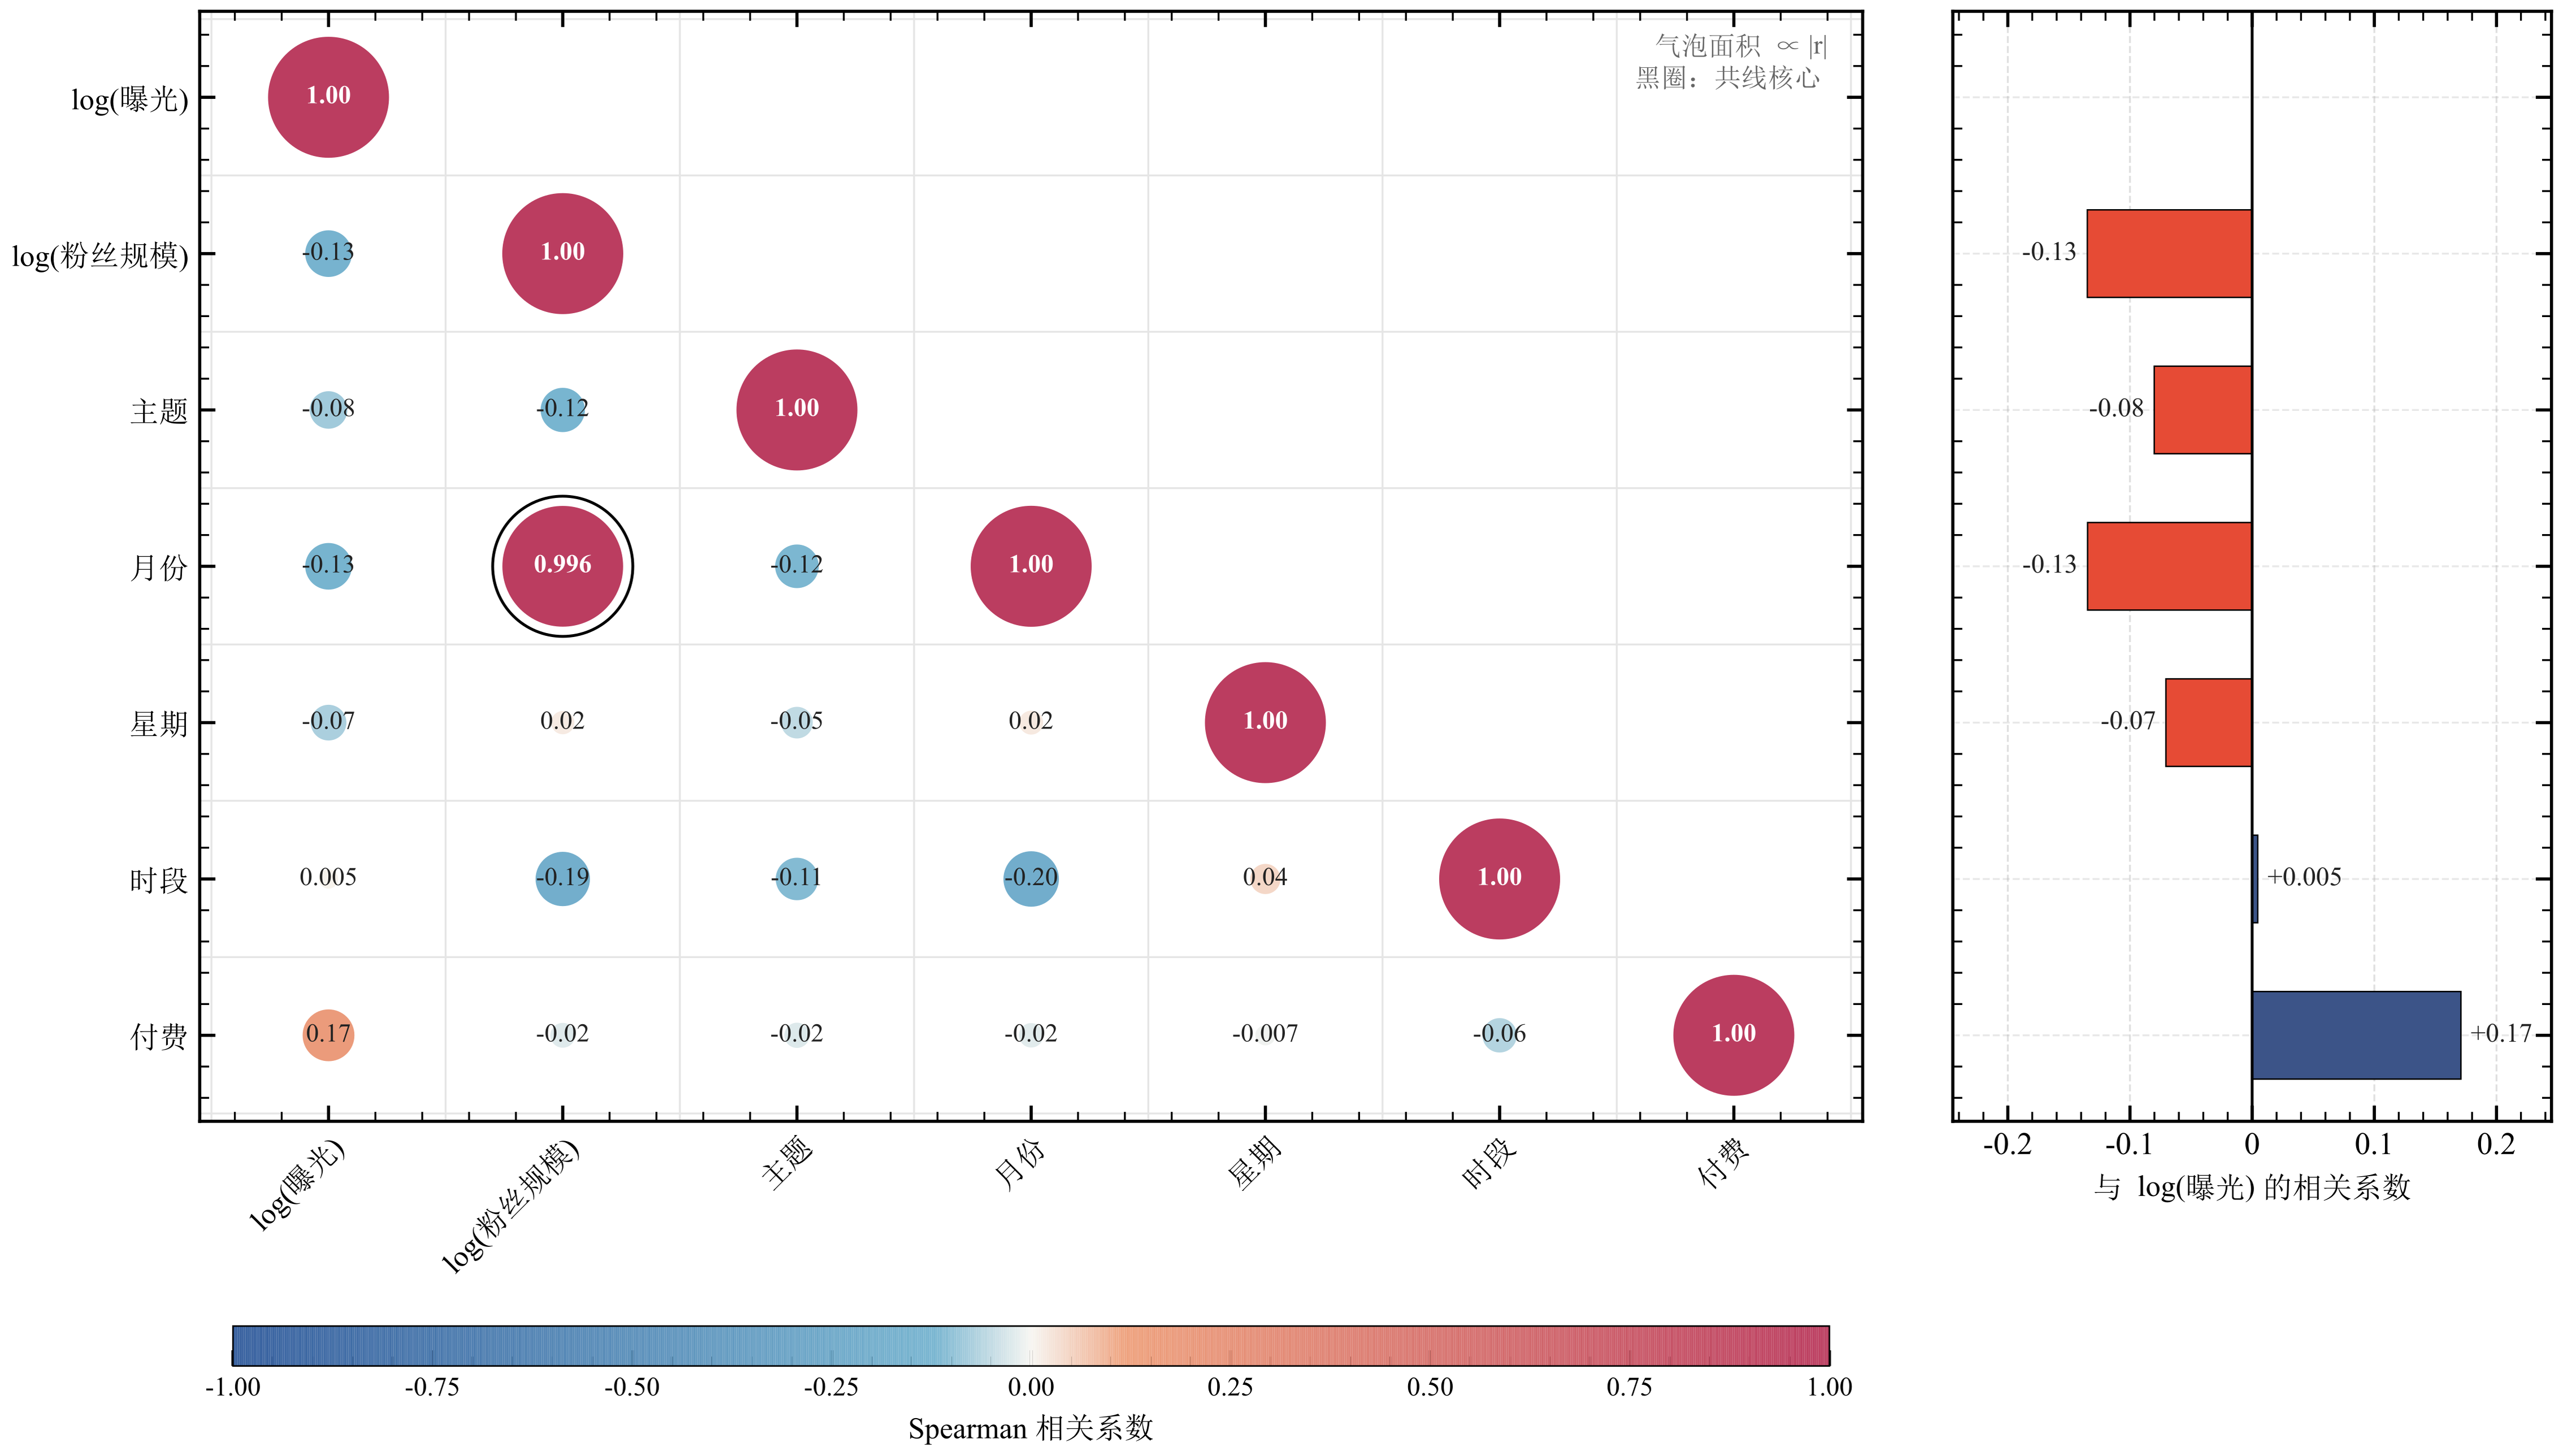
\includegraphics[width=0.82\textwidth]{../求解/问题一/结果/图3_相关系数热力图.png}
  \caption{变量间的 Spearman 相关矩阵与各变量对曝光的相关强度}
  \label{fig:q1_corr}
\end{figure}

图\ref{fig:q1_corr}的下三角气泡矩阵给出同一结论：除粉丝规模与月份那一格（黑圈标注，$r=0.996$）外，其余相关系数绝对值都不超过 0.20；右侧条形把各变量与曝光的相关系数单独列出，均为弱相关，说明单一变量都不足以解释曝光差异。


\begin{longtable}{>{\centering\arraybackslash}p{0.40\textwidth}>{\centering\arraybackslash}p{0.20\textwidth}>{\centering\arraybackslash}p{0.32\textwidth}}
  \caption{样本结构与共线指标}
  \label{tab:q1_desc} \\
  \toprule
  指标 & 数值 & 说明 \\
  \midrule
  \endfirsthead
  \caption{样本结构与共线指标（续）} \\
  \toprule
  指标 & 数值 & 说明 \\
  \midrule
  \endhead
  \bottomrule
  \endfoot
  样本量 & 500 & 每条记录对应一条帖子 \\
  变量数 & 8 & 7 个输入加 1 个输出 \\
  X1 唯一值数 & 90 & 同一粉丝数被多条帖子共享 \\
  X7 缺失数 & 1 & 占 0.2\%，仅第 499 行缺失 \\
  Y1 均值/中位/最大 & 29,586/9,051/1,110,282 & 最大值约为中位数的 122.67 倍 \\
  Y1 偏度/峰度 & 8.326/93.053 & 右偏、厚尾 \\
  log1p(Y1) 偏度/峰度 & 0.734/0.821 & 变换后接近对称 \\
  Pearson $r(X_1,X_4)$ & 0.941 & 线性同步程度高 \\
  Spearman $\rho(X_1,X_4)$ & 0.996 & 单调同步程度极高 \\
  $R^2(\log X_1\sim\text{月份})$ & 0.9917 & 99.17\% 的变异在月间 \\
  月内方差占比 & 0.0083 & 月内仅剩 0.83\% 的信息 \\
\end{longtable}

综合以上结果，数据理解的核心结论不是“粉丝规模影响曝光”，而是“粉丝规模与月份共同刻画了账号成长的时间维度，二者不能同时识别”。这一结论直接决定了后续的建模策略：以月份固定效应吸收规模趋势，把粉丝规模留作稳健性对照，而不是强行解释其系数。


% ════════════════════════════════════════════
% 数据清洗与特征整理（5.2）
% ════════════════════════════════════════════
\subsection{数据清洗与特征整理}

\subsubsection{缺失、异常与编码}

原始数据只有 1 条缺失、0 条重复，但类别变量的稀疏程度与因变量的重尾程度都超出线性回归的适用条件。付费标记 X7 仅在编号 499 的帖子缺失，占 0.2\%，该帖其余字段完整，删除会浪费一条有效信息，故采用众数填补，取值为 0，并附加填补标记以便追溯。7 个输入变量的取值范围全部落在字段说明之内，没有越界值；X6 的 0 时与 21 时没有帖子，实际只有 22 个取值；Y1 的 1,110,282 次是一条真实的病毒式传播记录，不作删除，改由 log1p 变换压缩其影响。

编码遵循“$K$ 个水平保留 $K-1$ 个哑变量”的规则。帖子类型以 Photo 为参照，保留 Status、Link、Video 三个哑变量；内容主题以主题 1 为参照，保留主题 2、主题 3 两个哑变量；月份与星期分别生成 11 个和 6 个哑变量，参照类为 1 月与周一；发帖小时合并为凌晨（0 至 5 时）、上午（6 至 11 时）与下午晚间（12 至 23 时）三组，并以上午为参照，三组分别有 196、193、111 条，均超过 100 条。加上常数项与付费标记，最终模型共需 $1+3+2+11+6+2+1=26$ 个参数。

图\ref{fig:q2_cat}显示，Photo 有 426 条，占 85.2\%，Status 45 条、Link 22 条、Video 仅 7 条；三类主题分别为 215、130、155 条，相对均衡；付费标记在填补后为自然 361 条、付费 139 条；发帖小时呈双峰分布，凌晨 3 时最多（105 条），上午 10 时次之（78 条）。视频与链接的样本量提示其估计精度有限，这一限制将在效应区间中直接体现。

\begin{figure}[ht]
  \centering
  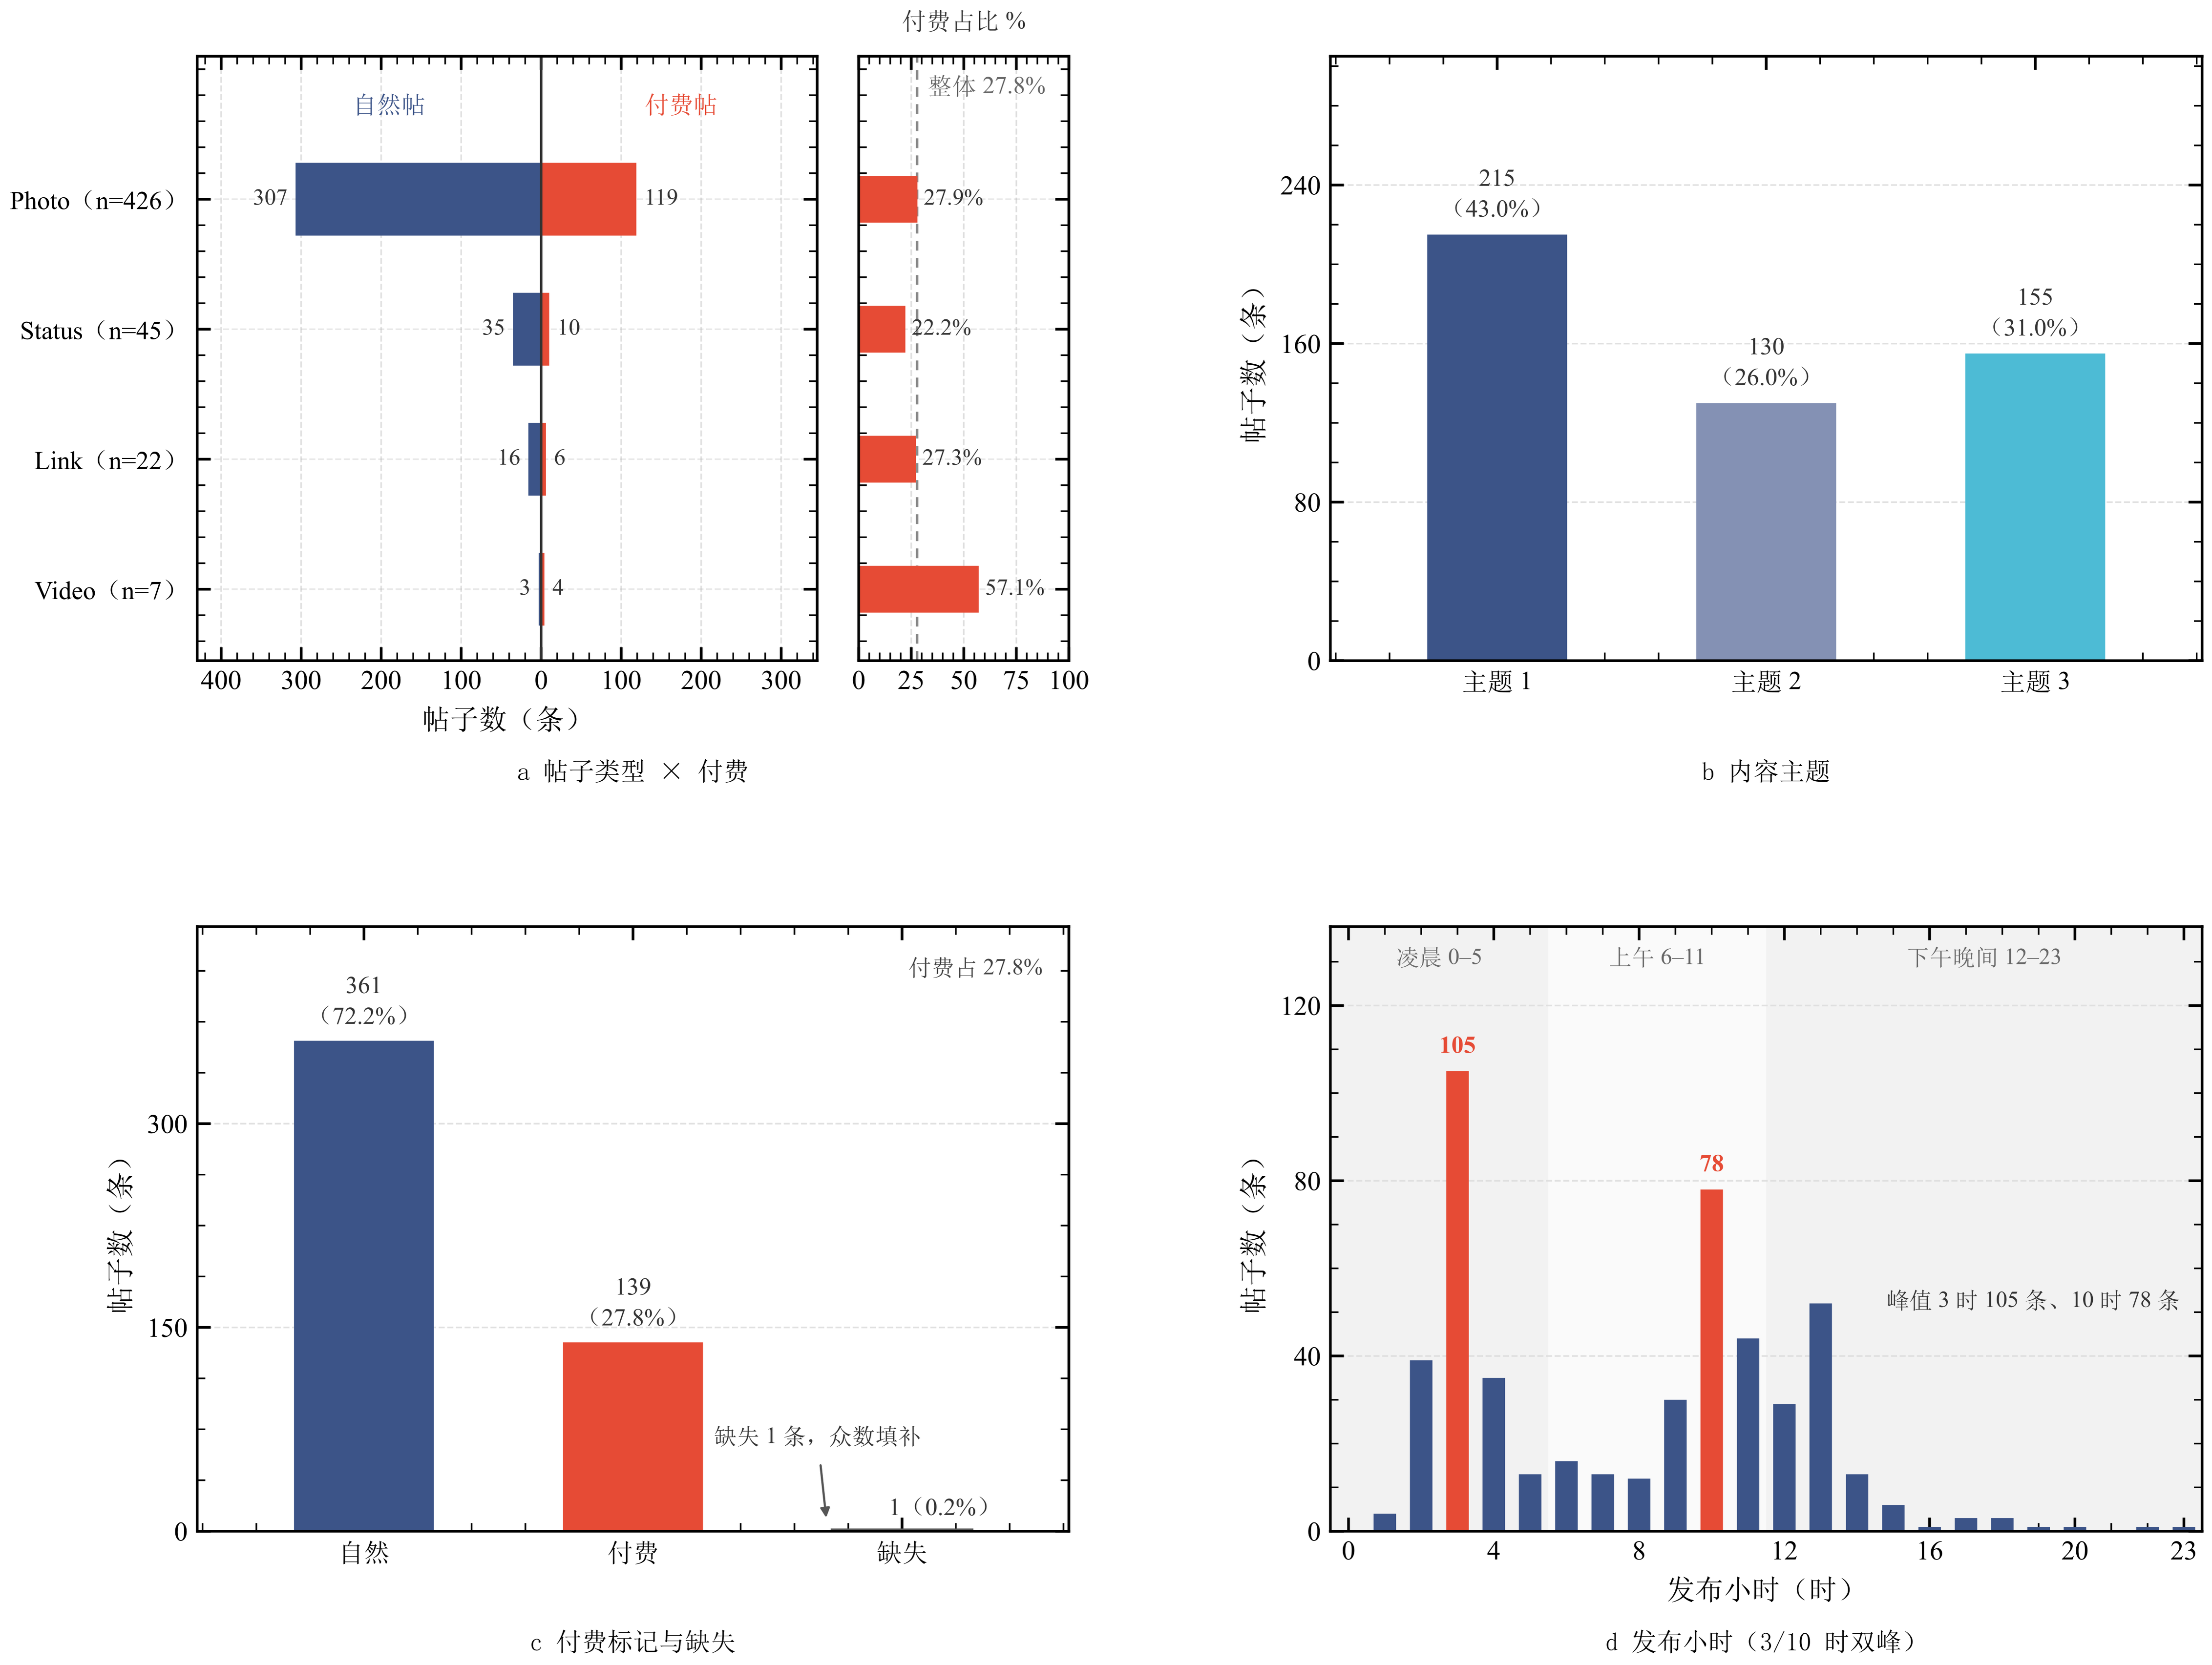
\includegraphics[width=0.70\textwidth]{../求解/问题二/结果/图4_类别结构与缺失.png}
  \caption{类别结构与缺失分布}
  \label{fig:q2_cat}
\end{figure}

表\ref{tab:q2_scheme}汇总了编码与变换方案。连续变量 X1 取对数，计数型因变量 Y1 取 log1p；名义变量 X2、X3 分别以 Photo、主题 1 为参照；月份、星期保留全部哑变量；时段合并为三组；X7 保持 0/1 数值。该方案共产生 26 个参数，与最终回归模型一致。

\begin{longtable}{>{\centering\arraybackslash}p{0.10\textwidth}>{\centering\arraybackslash}p{0.14\textwidth}>{\centering\arraybackslash}p{0.20\textwidth}>{\centering\arraybackslash}p{0.14\textwidth}>{\centering\arraybackslash}p{0.26\textwidth}}
  \caption{编码与变换方案}
  \label{tab:q2_scheme} \\
  \toprule
  变量 & 识别类型 & 编码或变换 & 基线或参照 & 解释 \\
  \midrule
  \endfirsthead
  \caption{编码与变换方案（续）} \\
  \toprule
  变量 & 识别类型 & 编码或变换 & 基线或参照 & 解释 \\
  \midrule
  \endhead
  \bottomrule
  \endfoot
  X1 & 连续 & $\log(X_1)$ & 无 & 粉丝规模弹性，压缩量级 \\
  X2 & 名义，4 类 & 独热编码，3 个哑变量 & Photo & 相对图片的曝光差异 \\
  X3 & 名义，3 类 & 独热编码，2 个哑变量 & 主题 1 & 相对主题 1 的曝光差异 \\
  X4 & 有序，12 类 & 独热编码，11 个哑变量 & 1 月 & 控制季节性与时间趋势 \\
  X5 & 有序，7 类 & 独热编码，6 个哑变量 & 周一 & 控制星期效应 \\
  X6 & 有序，24 类 & 合并 3 组，2 个哑变量 & 上午 & 控制时段效应，避免稀疏 \\
  X7 & 二元 & 0/1 数值 & 0，自然 & 付费的额外曝光 \\
  Y1 & 连续计数 & $\log(1+Y_1)$ & 无 & 压缩重尾，系数近似百分比 \\
\end{longtable}

\subsubsection{变换与敏感性}

曝光量为非负计数且右偏严重，采用 log1p 变换，即对曝光次数加 1 后取自然对数；加 1 保证曝光为零时有定义，本样本最小值为 570，实际不受影响。粉丝规模采用对数变换，把“每增加一人”改为“每增加 1\%”的弹性口径。两处变换只改变尺度，不改变样本排序。曝光量偏度由 8.3259 降至 0.7341，峰度由 93.0526 降至 0.8209，两项指标都回到接近正态的范围；最小值与最大值保持不变，说明变换没有删改任何观测。粉丝规模取对数后偏度由 $-0.9795$ 变为 $-1.1541$，左偏略有加强，这是粉丝数在高位堆积的必然结果，但其量级跨度被显著压缩，有利于数值稳定。

图\ref{fig:q2_trans}从分布形态与分位数两个角度对比变换效果。原始曝光量的直方图在 38 个等宽区间内有 396 条帖子落入首个区间，占 79.2\%；改用 30 个区间时为 414 条，占 82.8\%，两种分箱口径都显示首箱高度集中，其余观测拖出长尾。log1p 变换后的密度曲线与正态密度接近重合，Q--Q 图上的点也基本沿参考线分布，仅两端略有偏离。这说明 log1p 既保留了样本排序，又把极端值拉回了可建模的范围。

\begin{figure}[ht]
  \centering
  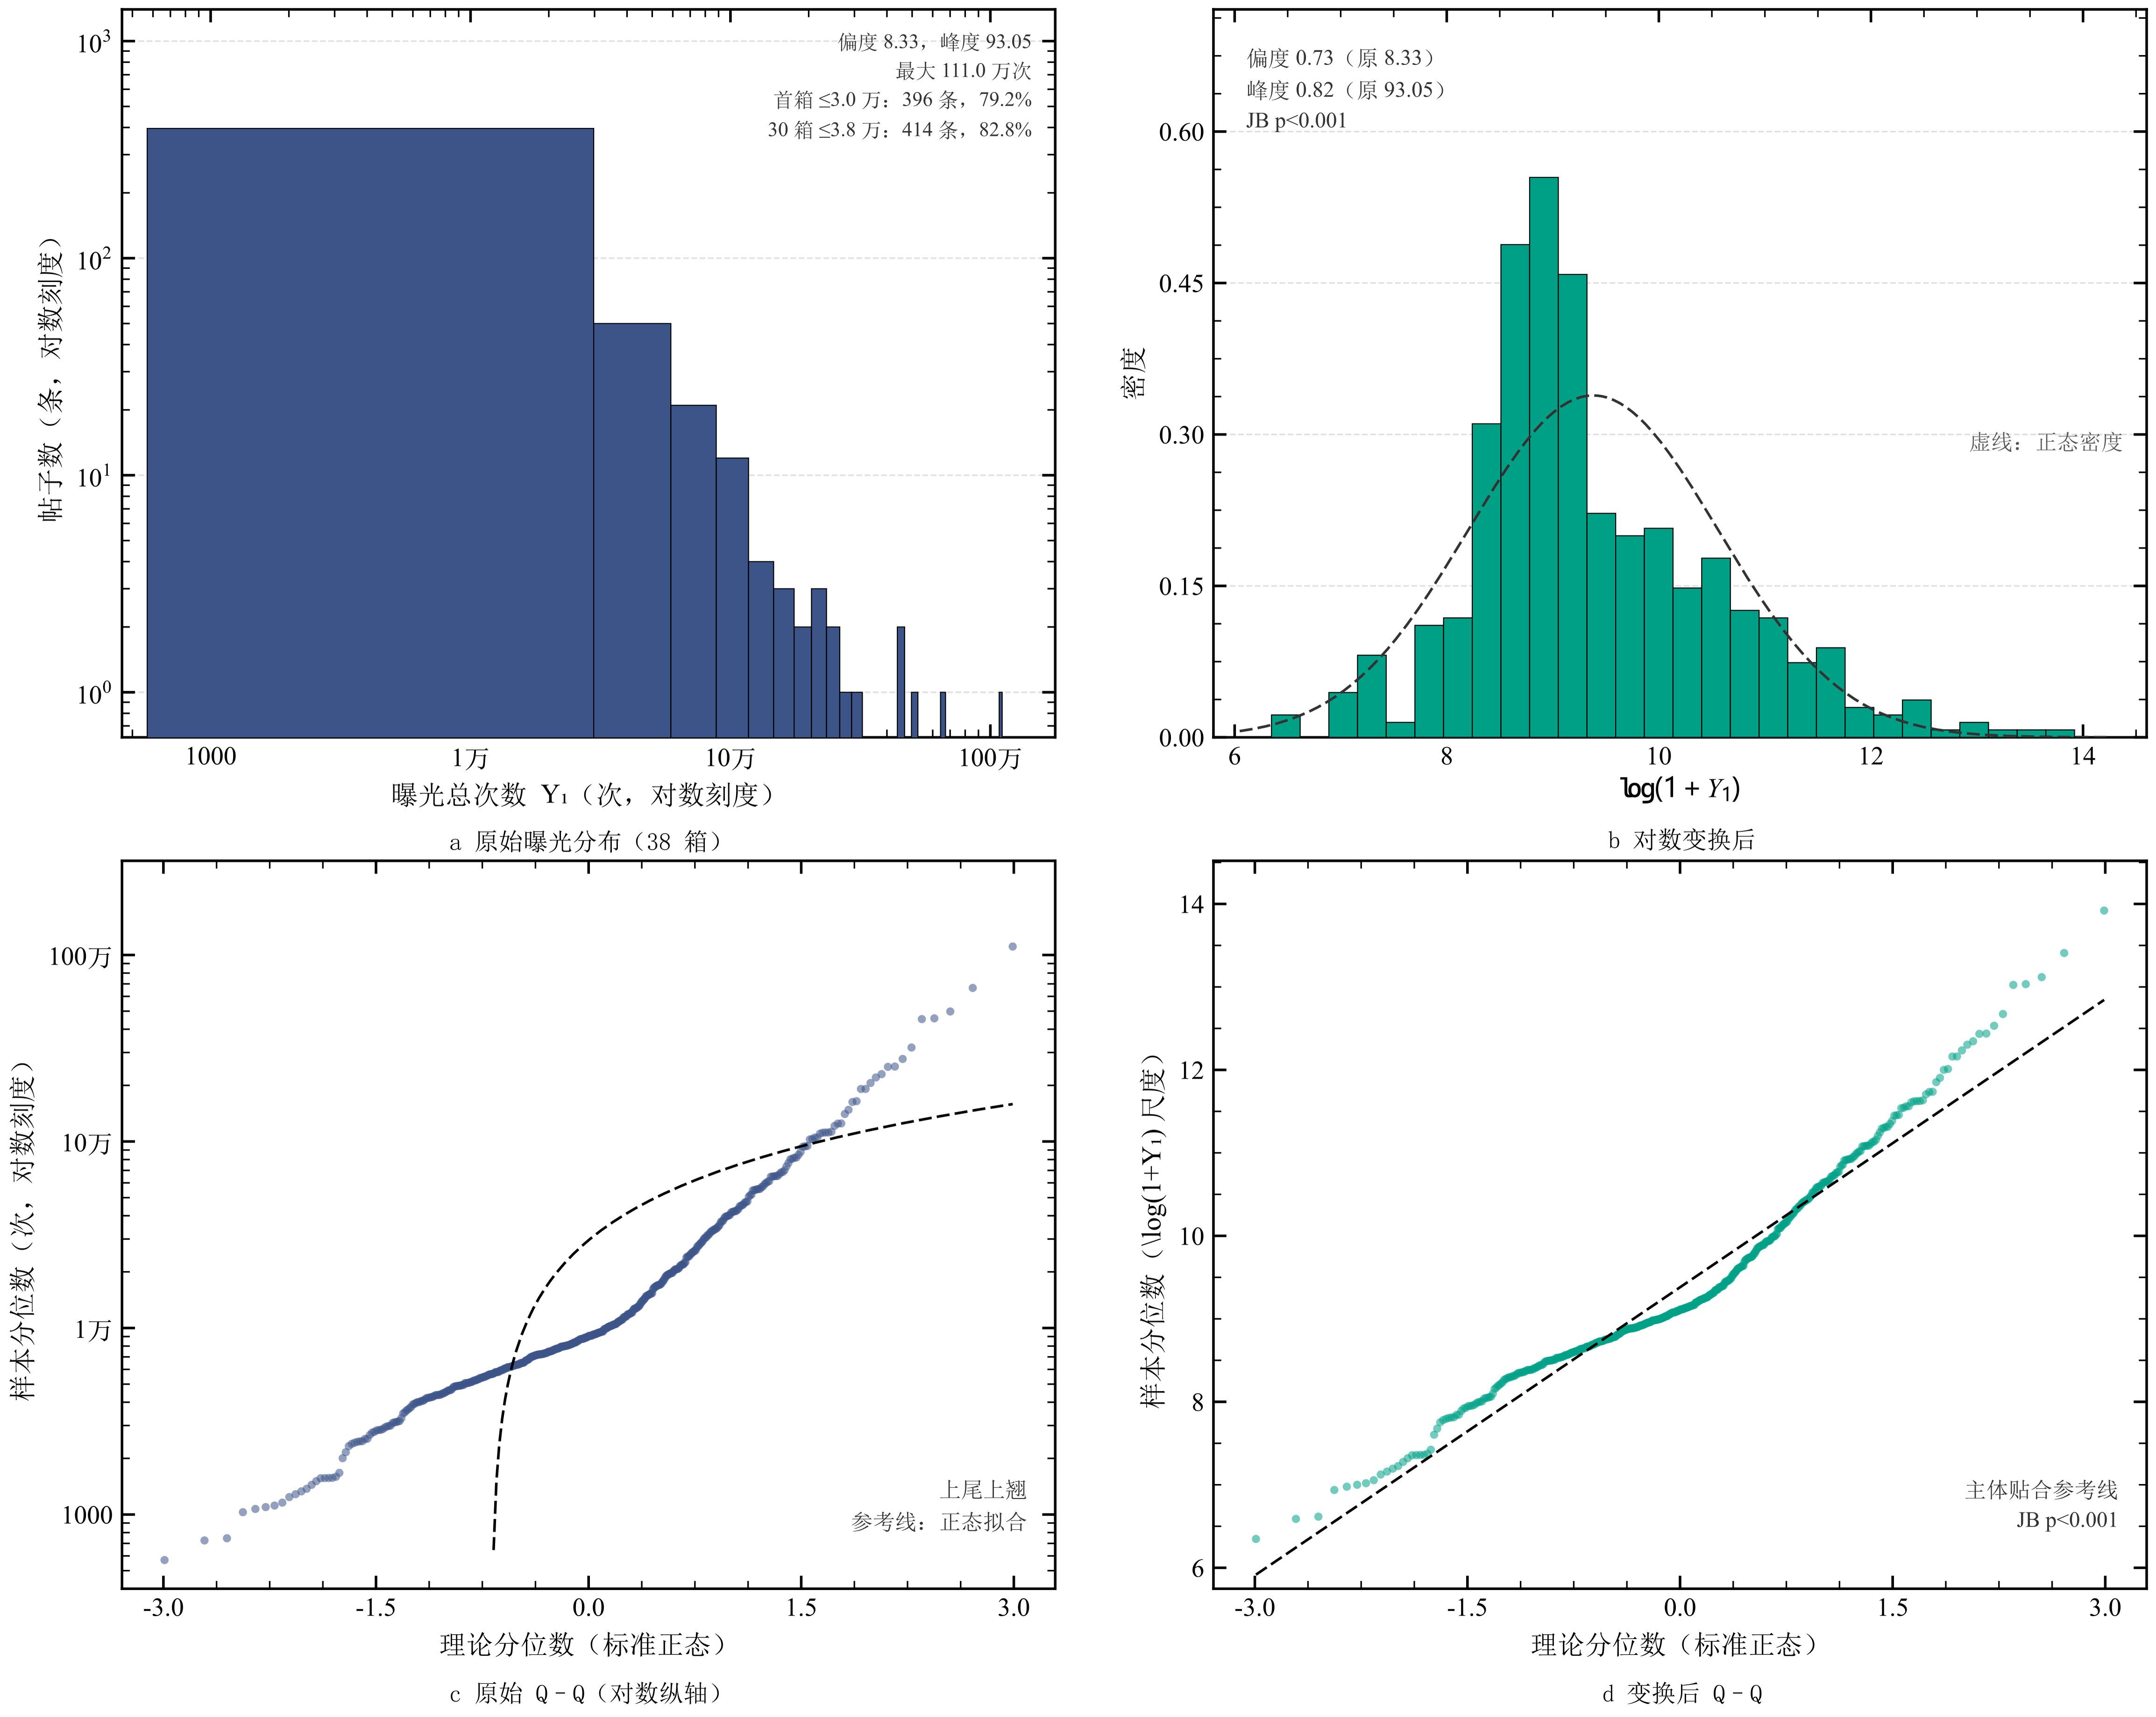
\includegraphics[width=0.70\textwidth]{../求解/问题二/结果/图5_变换前后分布.png}
  \caption{曝光量变换前后的分布与 Q--Q 图}
  \label{fig:q2_trans}
\end{figure}

在完成编码前，图\ref{fig:q2_time}先核对时间变量的经验结构。左上图把逐月发帖量与付费占比放在双轴上：发帖量在 1 月最低（25 条）、10 月最高（60 条），付费占比在 1 月的 16.0\% 与 4 月的 40.0\% 之间波动，既没有单边趋势，也不与发帖量同步。右上图给出逐月平均对数曝光的 95\% 置信带，2 月最高（10.13）、10 月最低（8.83），两月区间不重叠，说明月份既承载账号成长，也混入季节性的内容表现。左下图按星期排列，周四均值最高（9.74）、周日最低（9.06）；右下图按合并后的时段排列，上午最低（9.25）、下午晚间最高（9.50）。不过，星期与时段在控制月份、类型与主题后均不再显著（时段系数的 $p$ 值为 0.150 与 0.638），原始差异主要来自内容构成而非发布时间本身。基于这组证据，月份与星期保留为固定效应，24 小时合并为凌晨、上午、下午晚间三组，以避免稀疏小时带来不稳定估计。

\begin{figure}[ht]
  \centering
  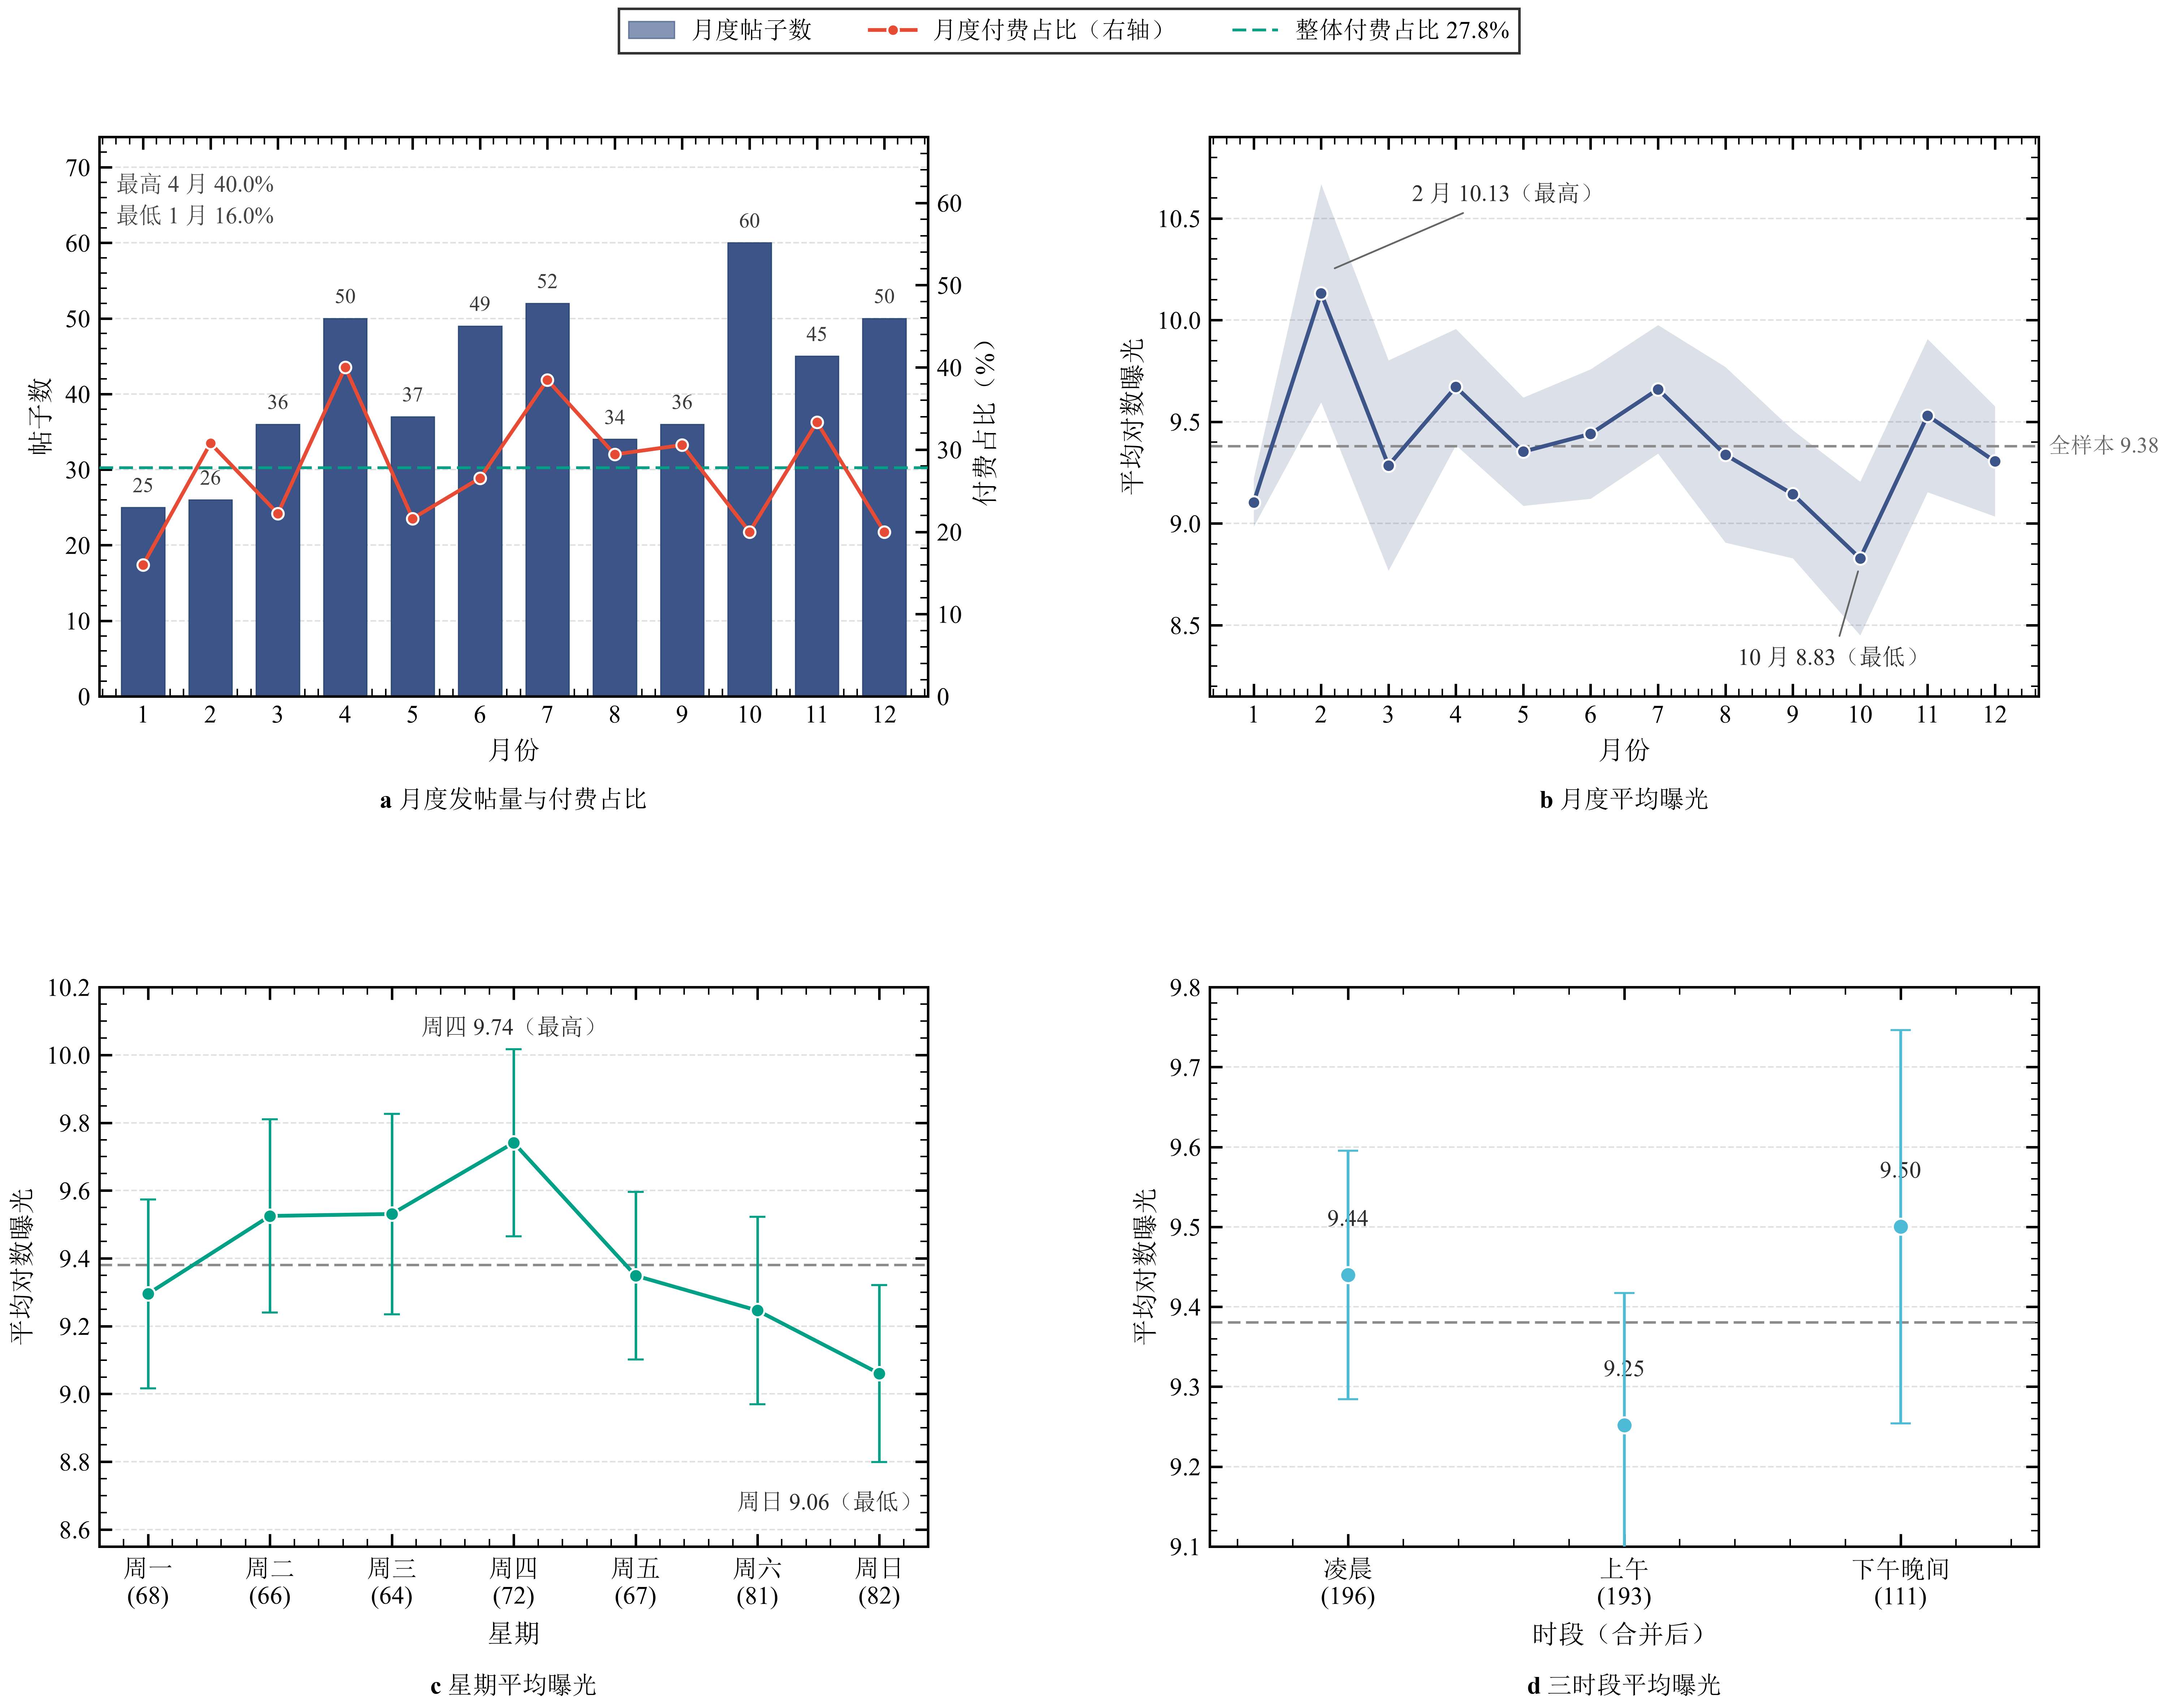
\includegraphics[width=0.70\textwidth]{../求解/临时产物/补充图2_时间结构.png}
  \caption{发帖量、付费占比与曝光的时间结构}
  \label{fig:q2_time}
\end{figure}

缺失处理的敏感性由系数对照给出。众数填补下付费系数为 0.3374、标准误 0.1115、样本量 500；删除缺失行后为 0.3363、标准误 0.1117、样本量 499，两者相差 0.0011，远小于预设的 0.01 阈值。可见填补方案既不改变系数方向，也不改变显著性判断，后续分析使用填补后的 500 条样本。清洗后的数据无缺失、无重复、无越界，类别编码完整，曝光量分布接近对称，可直接供回归建模与效应测算复用。


% ════════════════════════════════════════════
% 曝光量回归模型（5.3）
% ════════════════════════════════════════════
\subsection{曝光量回归模型}

\subsubsection{模型设定与估计}

本部分以 log1p 曝光量为因变量，构建包含粉丝规模、帖子类型、内容主题、月份、星期、时段与付费标记的全模型，并用 HC3 协方差矩阵处理异方差。模型写作
\begin{equation}
    y_i=\boldsymbol{x}_i^{\mathrm{T}}\boldsymbol{\beta}+\varepsilon_i,
    \qquad i=1,2,\ldots,n,
\end{equation}
其中 $y_i=\log(1+Y_i)$，$\boldsymbol{\beta}$ 为待估系数，$\varepsilon_i$ 为随机扰动。系数由最小二乘估计；在经典假定下，系数协方差等于扰动方差乘以设计矩阵交叉乘积的逆。曝光量重尾使残差方差随拟合值变化，经典标准误会低估不确定性，因此采用 White 异方差稳健估计的 HC3 修正：第 $i$ 个残差平方除以 $(1-h_{ii})^2$ 后加权，$h_{ii}$ 为该观测的杠杆值\cite{white1980}。该修正不改变系数点估计，只修正标准误，系数表可以与经典结果直接对照。

为分离共线的影响，设置五个递进模型。M0 只含常数项，作为均值基线；M1 为全模型，同时含粉丝规模对数与 11 个月份哑变量；M2 剔除粉丝规模、保留月份固定效应；M3 保留粉丝规模、剔除月份；M4 同时含粉丝规模与线性月份项。M2 用月份固定效应吸收粉丝规模的累积趋势，是本报告的最终解释模型；M1、M3、M4 用于检验付费与内容类型的系数是否随设定改变。

图\ref{fig:q3_score}以评分表形式比较五种模型。评分由十折交叉验证的 $R^2$ 均值减去 0.1 倍折间标准差得到，兼顾预测精度与稳定性。M2 的得分为 0.0909，居五者之首；M4 为 0.0888、M1 为 0.0871、M3 为 0.0848，均值基线 M0 为 $-0.0238$。M2 的样本内 $R^2$ 为 0.2068、调整 $R^2$ 为 0.1650、残差标准误 1.0765，十折交叉验证 $R^2$ 为 0.1010、RMSE 1.1007、MAE 0.8328；M1 的样本内 $R^2$ 几乎相同（0.2069），但多一个参数、调整 $R^2$ 略低（0.1633），交叉验证 $R^2$ 也略低（0.0972）。这说明剔除粉丝规模没有损失解释力，反而改善了样本外表现。

\begin{figure}[ht]
  \centering
  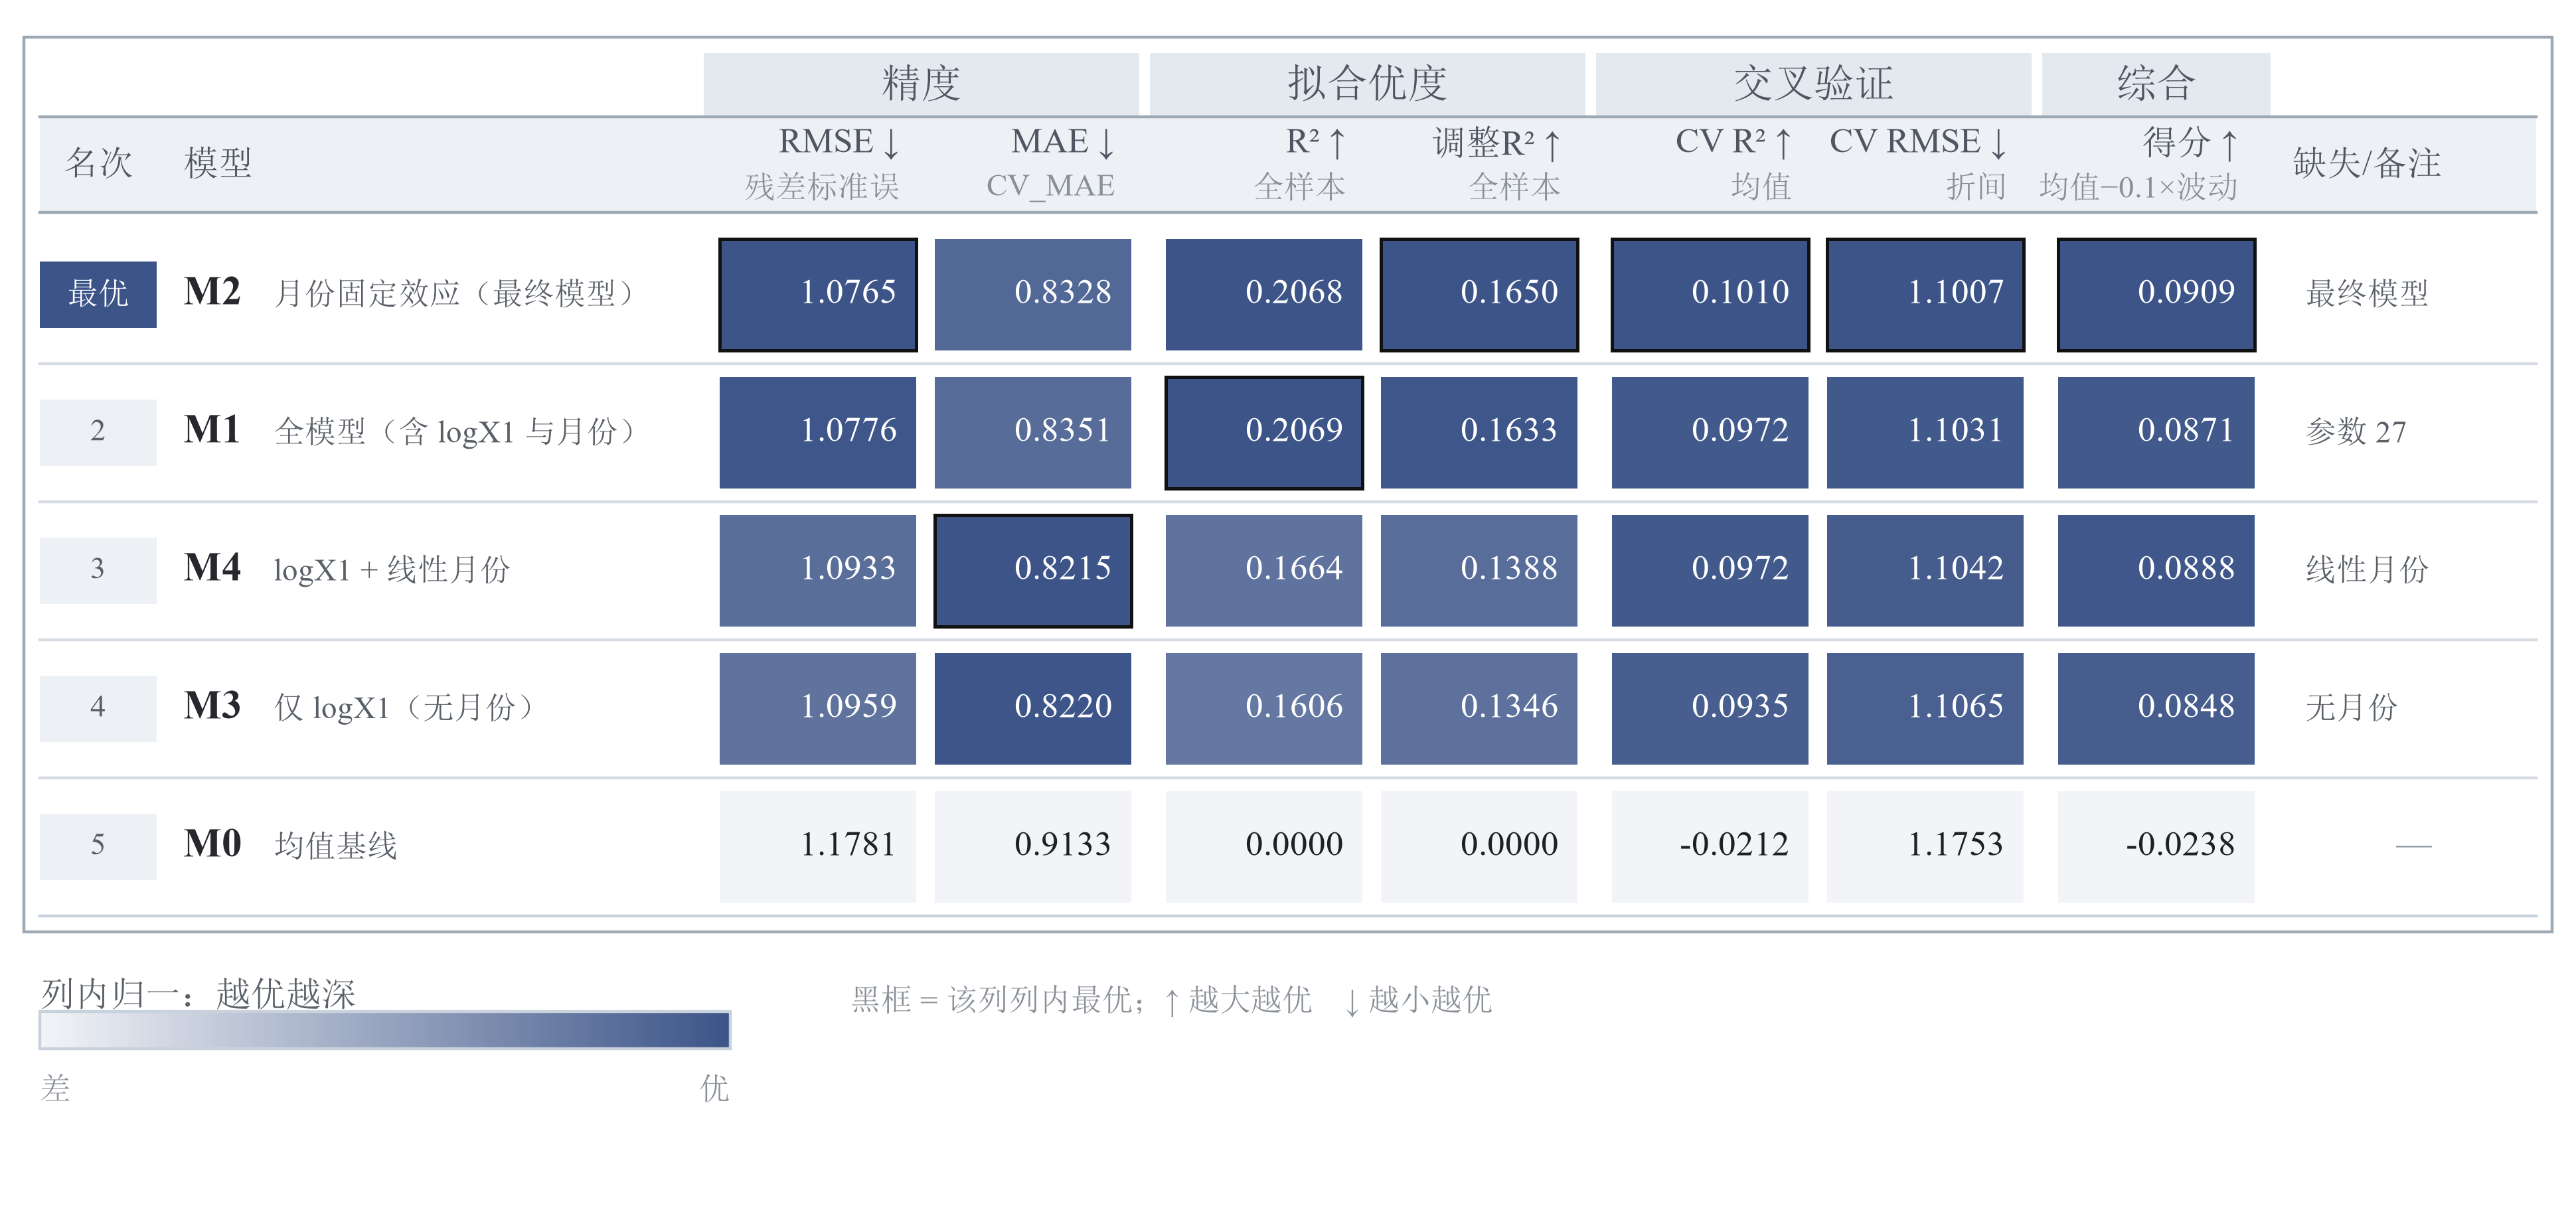
\includegraphics[width=0.74\textwidth]{../求解/问题三/结果/图15_模型绩效评分表.png}
  \caption{五种模型的精度、拟合优度、交叉验证与综合得分}
  \label{fig:q3_score}
\end{figure}

\subsubsection{共线与残差诊断}

表\ref{tab:q3_diag}把共线与残差证据集中列出。M1 的最大 VIF 为 142.99，出现在 10 月；粉丝规模的 VIF 为 124.91；标准化条件数为 48.52，超过 30 的严重阈值。月份哑变量的 VIF 自 3 月起快速上升，到 10 月达到峰值，与粉丝规模的 VIF 互为镜像，说明二者在争抢同一段变异。增量 $F$ 检验显示，在已含月份固定效应的模型中加入粉丝规模，$F$ 值仅 0.0495、$p$ 值 0.824，几乎不增加任何解释力。M2 剔除粉丝规模后，最大 VIF 降至 3.232、条件数降至 6.356，共线问题基本消除；GVIF 方面，粉丝规模的 $\mathrm{GVIF}^{1/2}$ 为 11.176，远超阈值 2.24，其余变量组均低于 1.28。

\begin{longtable}{>{\centering\arraybackslash}p{0.28\textwidth}>{\centering\arraybackslash}p{0.23\textwidth}>{\centering\arraybackslash}p{0.11\textwidth}>{\centering\arraybackslash}p{0.26\textwidth}}
  \caption{共线性与残差诊断}
  \label{tab:q3_diag} \\
  \toprule
  诊断项 & 对象 & 数值 & 判断 \\
  \midrule
  \endfirsthead
  \caption{共线性与残差诊断（续）} \\
  \toprule
  诊断项 & 对象 & 数值 & 判断 \\
  \midrule
  \endhead
  \bottomrule
  \endfoot
  M1 最大 VIF & 全部解释变量 & 142.994 & 超过 10，严重共线 \\
  M1 VIF & $\log X_1$ & 124.905 & 超过 10，严重共线 \\
  M1 条件数 & 标准化设计矩阵 & 48.519 & 超过 30，数值不稳定 \\
  增量 $F$ 统计量 & 在 M2 中加入 $\log X_1$ & 0.0495 & 增量贡献极小 \\
  增量 $F$ 检验 $p$ 值 & 同上 & 0.824 & 不显著，系数不可识别 \\
  $R^2(\log X_1\sim\text{月份})$ & 月间趋势 & 0.9917 & 粉丝规模几乎由月份决定 \\
  月内方差占比 & 组内变异 & 0.0083 & 低于 0.05，月内信息不足 \\
  M2 最大 VIF & 全部解释变量 & 3.232 & 低于 5，可接受 \\
  M2 条件数 & 标准化设计矩阵 & 6.356 & 低于 30，通过 \\
  $\mathrm{GVIF}^{1/2}$ & $\log X_1$ & 11.176 & 超过阈值 2.24 \\
  $\mathrm{GVIF}^{1/2}$ & 其余变量组 & 1.018--1.278 & 均低于 2.24 \\
  Jarque--Bera & M2 残差 & 120.360 & $p<0.001$，残差非正态 \\
  Breusch--Pagan & M2 残差 & 54.737 & $p=0.0005$，存在异方差 \\
  White & M2 残差 & 266.519 & $p=0.030$，存在异方差 \\
  Ramsey RESET & M2 & 2.845 & $p=0.059$，未检出设定误差 \\
  Durbin--Watson & M2 & 2.052 & 接近 2，无强自相关 \\
  Cook 距离最大值 & M2 & 0.0377 & 远小于 1，无强影响点 \\
  高杠杆点个数 & M2 & 10 & 阈值 $2p/n=0.104$ \\
\end{longtable}

图\ref{fig:q3_vif}直观展示共线处理前后的差异。左图中粉丝规模与 6 月至 12 月的月份哑变量全部越过 10 的参考线，最高接近 143；右图中最终模型的全部变量都落在 5 以下，最高的月份变量仅为 3.23。这说明剔除粉丝规模并非损失信息，而是把重复计数的时间维度合并为一个，使剩余系数可以稳定估计。

\begin{figure}[ht]
  \centering
  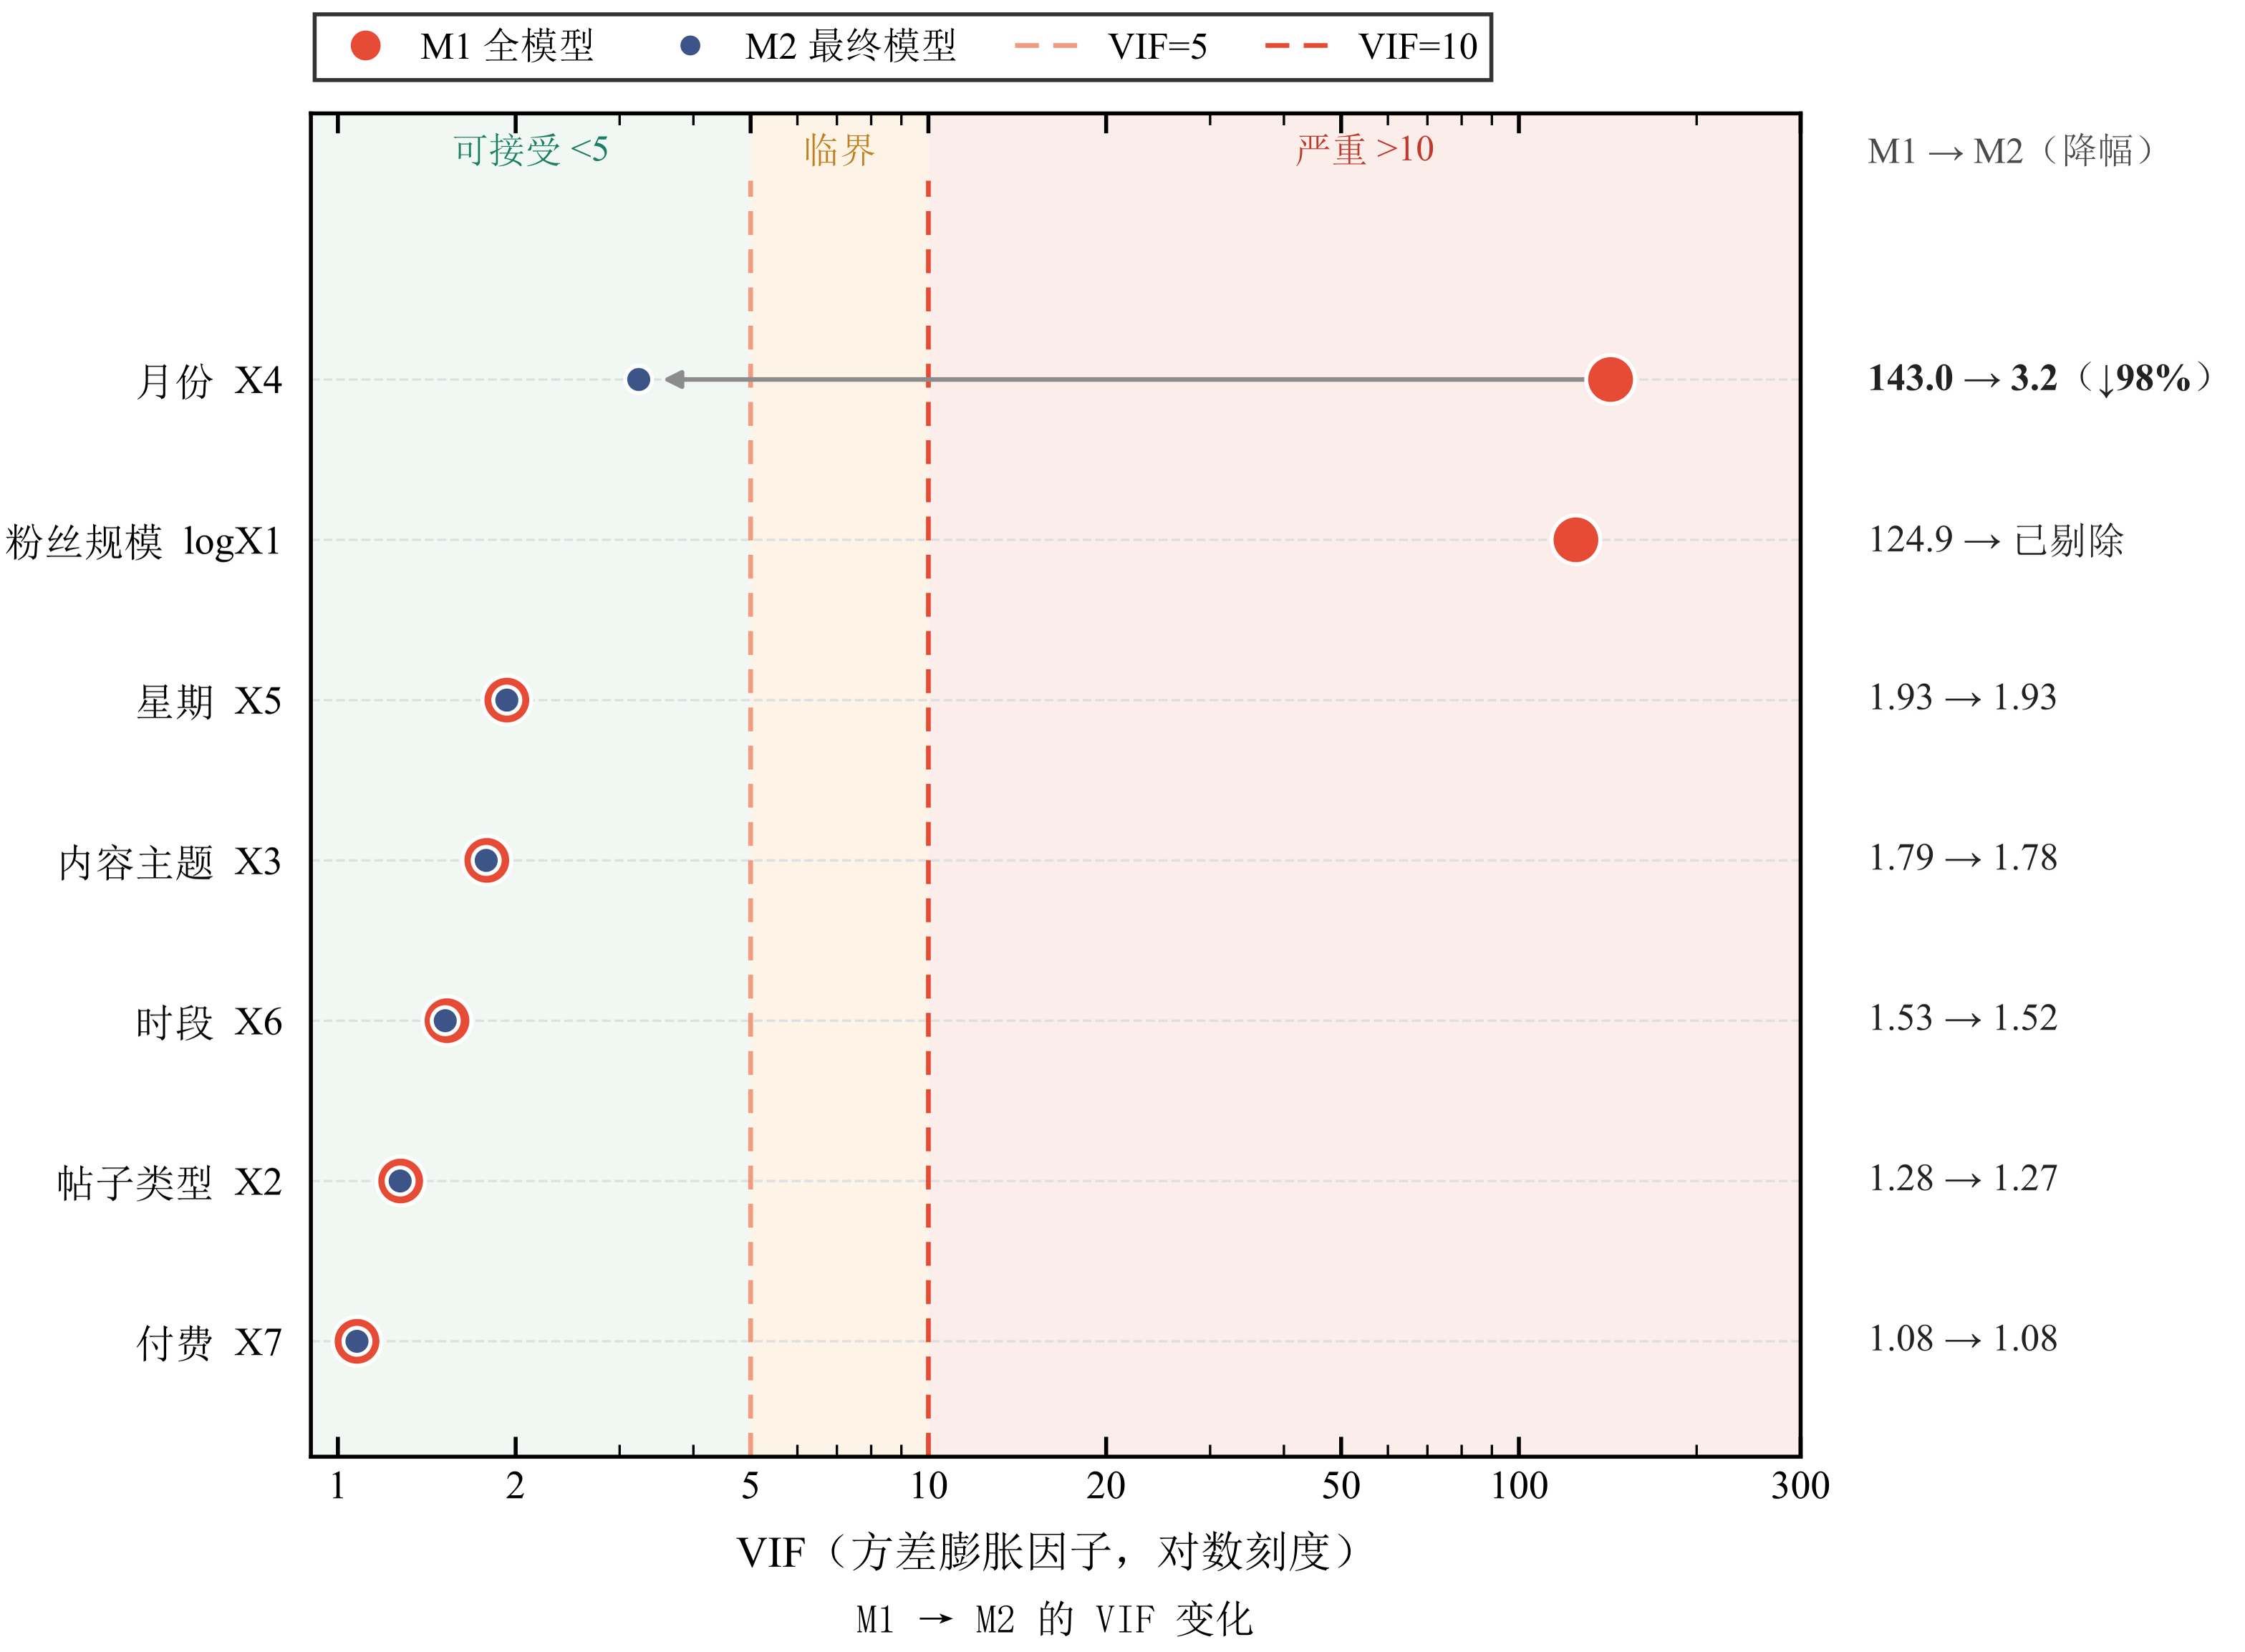
\includegraphics[width=0.68\textwidth]{../求解/问题三/结果/图7_共线性诊断.png}
  \caption{全模型与最终模型的方差膨胀因子}
  \label{fig:q3_vif}
\end{figure}

最终模型 M2 的系数如表\ref{tab:q3_final}所示。常数项 9.2468 对应参照组合（Photo、主题 1、1 月、周一、上午、自然）的基线对数曝光。Status 的系数为 1.1538、$p$ 值小于 0.001，折算为 $e^{1.1538}=3.17$ 倍；Video 为 1.5896、$p$ 值 0.0001，折算为 4.90 倍；Link 为 0.1215、$p$ 值 0.643，折算为 1.13 倍且不显著。主题 2 与主题 3 分别为 $-0.4784$ 与 $-0.3147$，折算为 0.62 倍与 0.73 倍。付费系数为 0.3374、$p$ 值 0.005，折算为 1.40 倍。月份与星期的系数为控制变量，完整估计见表\ref{tab:q3_final}；其中 2 月、4 月为正，10 月为负，其余月份与全部星期、时段系数均不显著。

\begin{longtable}{>{\centering\arraybackslash}p{0.17\textwidth}>{\centering\arraybackslash}p{0.085\textwidth}>{\centering\arraybackslash}p{0.085\textwidth}>{\centering\arraybackslash}p{0.07\textwidth}>{\centering\arraybackslash}p{0.07\textwidth}>{\centering\arraybackslash}p{0.08\textwidth}>{\centering\arraybackslash}p{0.08\textwidth}>{\centering\arraybackslash}p{0.08\textwidth}}
  \caption{最终模型 M2 系数表}
  \label{tab:q3_final} \\
  \toprule
  变量 & 系数 & HC3\newline 标准误 & $t$ 值 & $p$ 值 & CI 下限 & CI 上限 & VIF \\
  \midrule
  \endfirsthead
  \caption{最终模型 M2 系数表（续）} \\
  \toprule
  变量 & 系数 & HC3\newline 标准误 & $t$ 值 & $p$ 值 & CI 下限 & CI 上限 & VIF \\
  \midrule
  \endhead
  \bottomrule
  \endfoot
  常数项 & 9.247 & 0.205 & 45.062 & $<$0.001 & 8.844 & 9.650 & — \\
  类型 Status & 1.154 & 0.124 & 9.339 & $<$0.001 & 0.911 & 1.397 & 1.275 \\
  类型 Link & 0.122 & 0.262 & 0.464 & 0.643 & $-0.393$ & 0.636 & 1.136 \\
  类型 Video & 1.590 & 0.402 & 3.958 & $<$0.001 & 0.800 & 2.379 & 1.063 \\
  主题 2 & $-0.478$ & 0.135 & $-3.540$ & $<$0.001 & $-0.744$ & $-0.213$ & 1.783 \\
  主题 3 & $-0.315$ & 0.134 & $-2.353$ & 0.019 & $-0.578$ & $-0.052$ & 1.527 \\
  月份 2 & 0.877 & 0.304 & 2.886 & 0.004 & 0.280 & 1.473 & 2.039 \\
  月份 3 & $-0.041$ & 0.310 & $-0.134$ & 0.894 & $-0.650$ & 0.567 & 2.543 \\
  月份 4 & 0.381 & 0.177 & 2.154 & 0.032 & 0.033 & 0.728 & 2.835 \\
  月份 5 & 0.191 & 0.171 & 1.116 & 0.265 & $-0.145$ & 0.527 & 2.362 \\
  月份 6 & 0.149 & 0.185 & 0.806 & 0.421 & $-0.214$ & 0.513 & 2.820 \\
  月份 7 & 0.313 & 0.190 & 1.648 & 0.100 & $-0.060$ & 0.687 & 2.971 \\
  月份 8 & 0.112 & 0.248 & 0.451 & 0.652 & $-0.376$ & 0.600 & 2.306 \\
  月份 9 & $-0.126$ & 0.188 & $-0.671$ & 0.503 & $-0.495$ & 0.243 & 2.426 \\
  月份 10 & $-0.471$ & 0.214 & $-2.206$ & 0.028 & $-0.891$ & $-0.051$ & 3.232 \\
  月份 11 & 0.036 & 0.196 & 0.181 & 0.856 & $-0.349$ & 0.420 & 2.808 \\
  月份 12 & $-0.101$ & 0.164 & $-0.616$ & 0.538 & $-0.424$ & 0.222 & 2.851 \\
  星期 2 & 0.094 & 0.198 & 0.475 & 0.635 & $-0.295$ & 0.482 & 1.759 \\
  星期 3 & $-0.019$ & 0.192 & $-0.099$ & 0.921 & $-0.396$ & 0.358 & 1.768 \\
  星期 4 & 0.259 & 0.208 & 1.241 & 0.215 & $-0.151$ & 0.668 & 1.847 \\
  星期 5 & $-0.093$ & 0.177 & $-0.525$ & 0.600 & $-0.441$ & 0.255 & 1.795 \\
  星期 6 & $-0.161$ & 0.185 & $-0.868$ & 0.386 & $-0.525$ & 0.203 & 1.932 \\
  星期 7 & $-0.221$ & 0.175 & $-1.263$ & 0.207 & $-0.566$ & 0.123 & 1.897 \\
  时段 凌晨 & 0.164 & 0.114 & 1.443 & 0.150 & $-0.060$ & 0.388 & 1.318 \\
  时段 下午晚间 & 0.075 & 0.160 & 0.471 & 0.638 & $-0.238$ & 0.389 & 1.520 \\
  付费 & 0.337 & 0.120 & 2.823 & 0.005 & 0.103 & 0.572 & 1.077 \\
\end{longtable}

图\ref{fig:q3_forest}以森林图形式展示主效应。点估计按正负与显著性着色，横轴为 log1p 尺度，右侧标注折算后的倍数与 95\% 置信区间。Status 与 Video 的区间完全位于 0 的右侧，主题 2 与主题 3 的区间完全位于 0 的左侧，付费的区间也整体为正；Link 的区间跨越 0，对应 $p$ 值 0.643。Video 的区间最宽，上界接近 2.38，这是仅 7 条视频帖带来的必然结果，解读时应强调方向而非精确倍数。

\begin{figure}[ht]
  \centering
  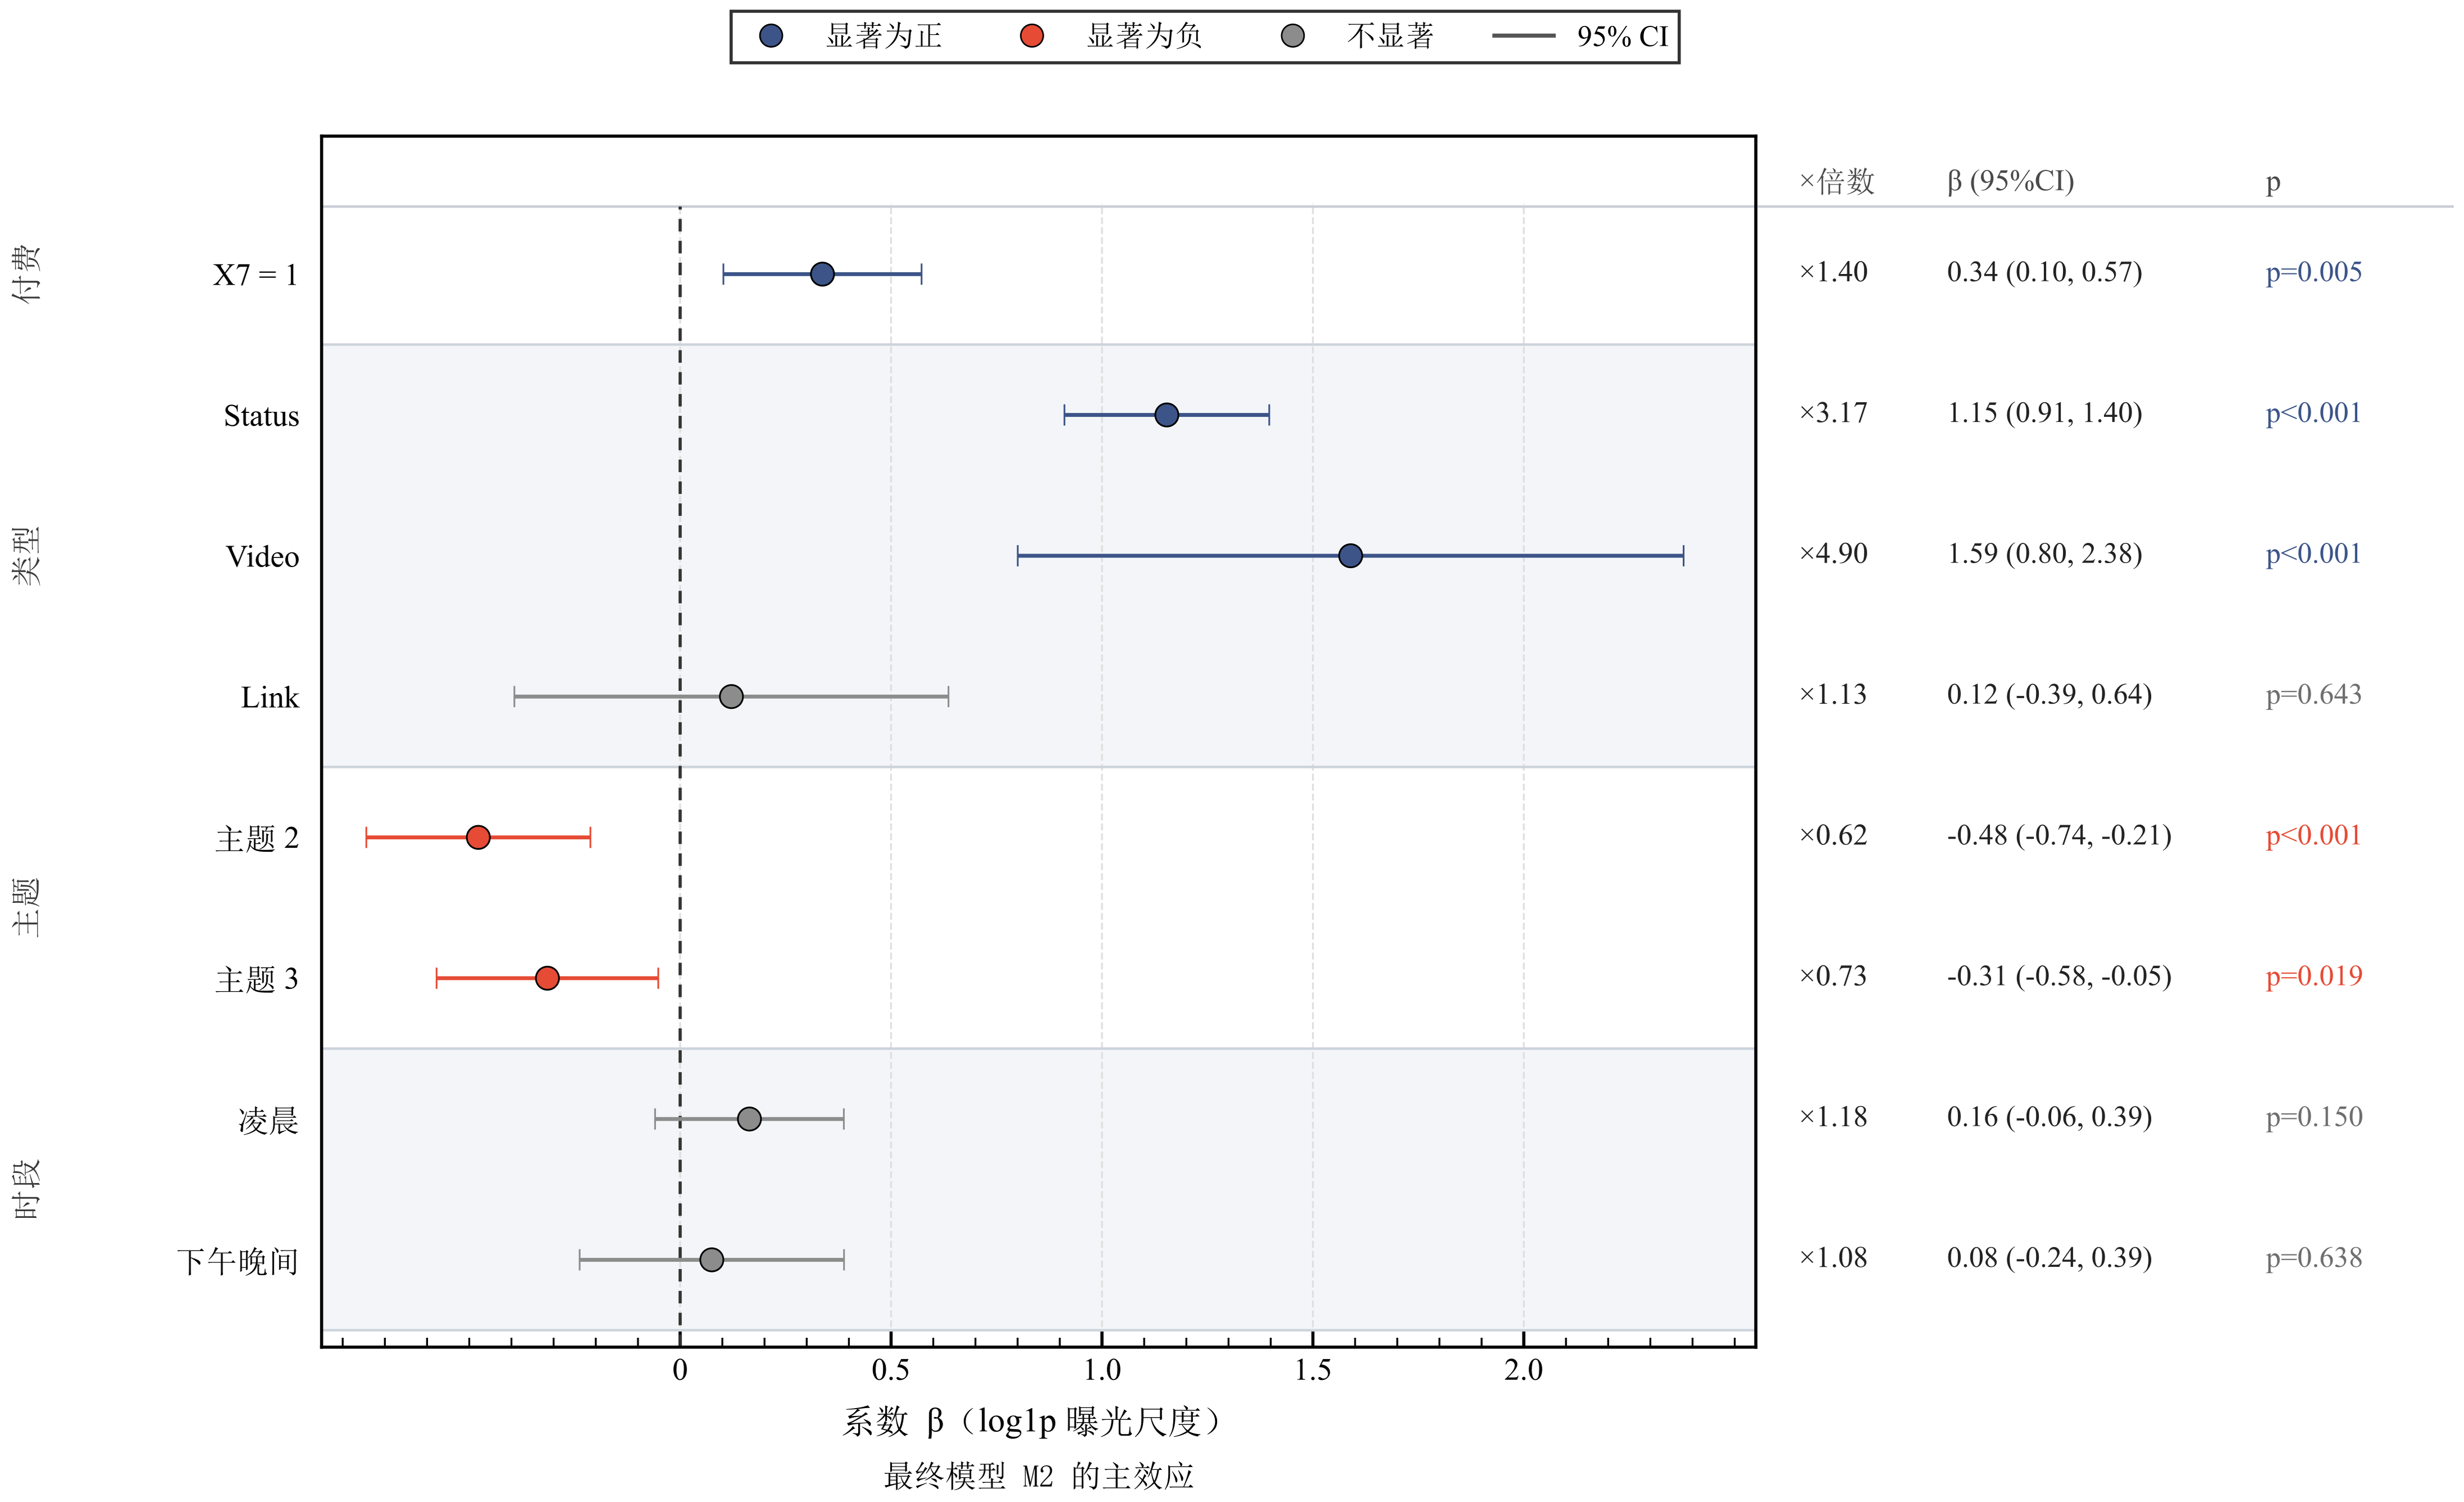
\includegraphics[width=0.70\textwidth]{../求解/问题三/结果/图6_最终模型系数森林图.png}
  \caption{最终模型主效应系数与 95\% 置信区间}
  \label{fig:q3_forest}
\end{figure}

表\ref{tab:q3_diag}的下半部分报告残差诊断。Jarque--Bera 统计量为 120.36、$p$ 值小于 0.001，残差仍偏离正态；Breusch--Pagan 统计量为 54.74、$p$ 值 0.0005，White 统计量 266.52、$p$ 值 0.030，两项都拒绝同方差。这正是采用 HC3 标准误的理由。Ramsey RESET 的 $F$ 值为 2.845、$p$ 值 0.059，在 5\% 水平未检出函数形式误设；Durbin--Watson 为 2.052，接近 2；Cook 距离最大值为 0.0377，远小于 1，说明没有单条帖子主导估计。按 $4/n=0.0080$ 的常用参考线，有 30 个观测超过该线，但最大 Cook 距离仍不足 0.04，属于局部影响而非全局主导；杠杆值超过 $2p/n=0.104$ 的观测有 10 个。

\begin{figure}[ht]
  \centering
  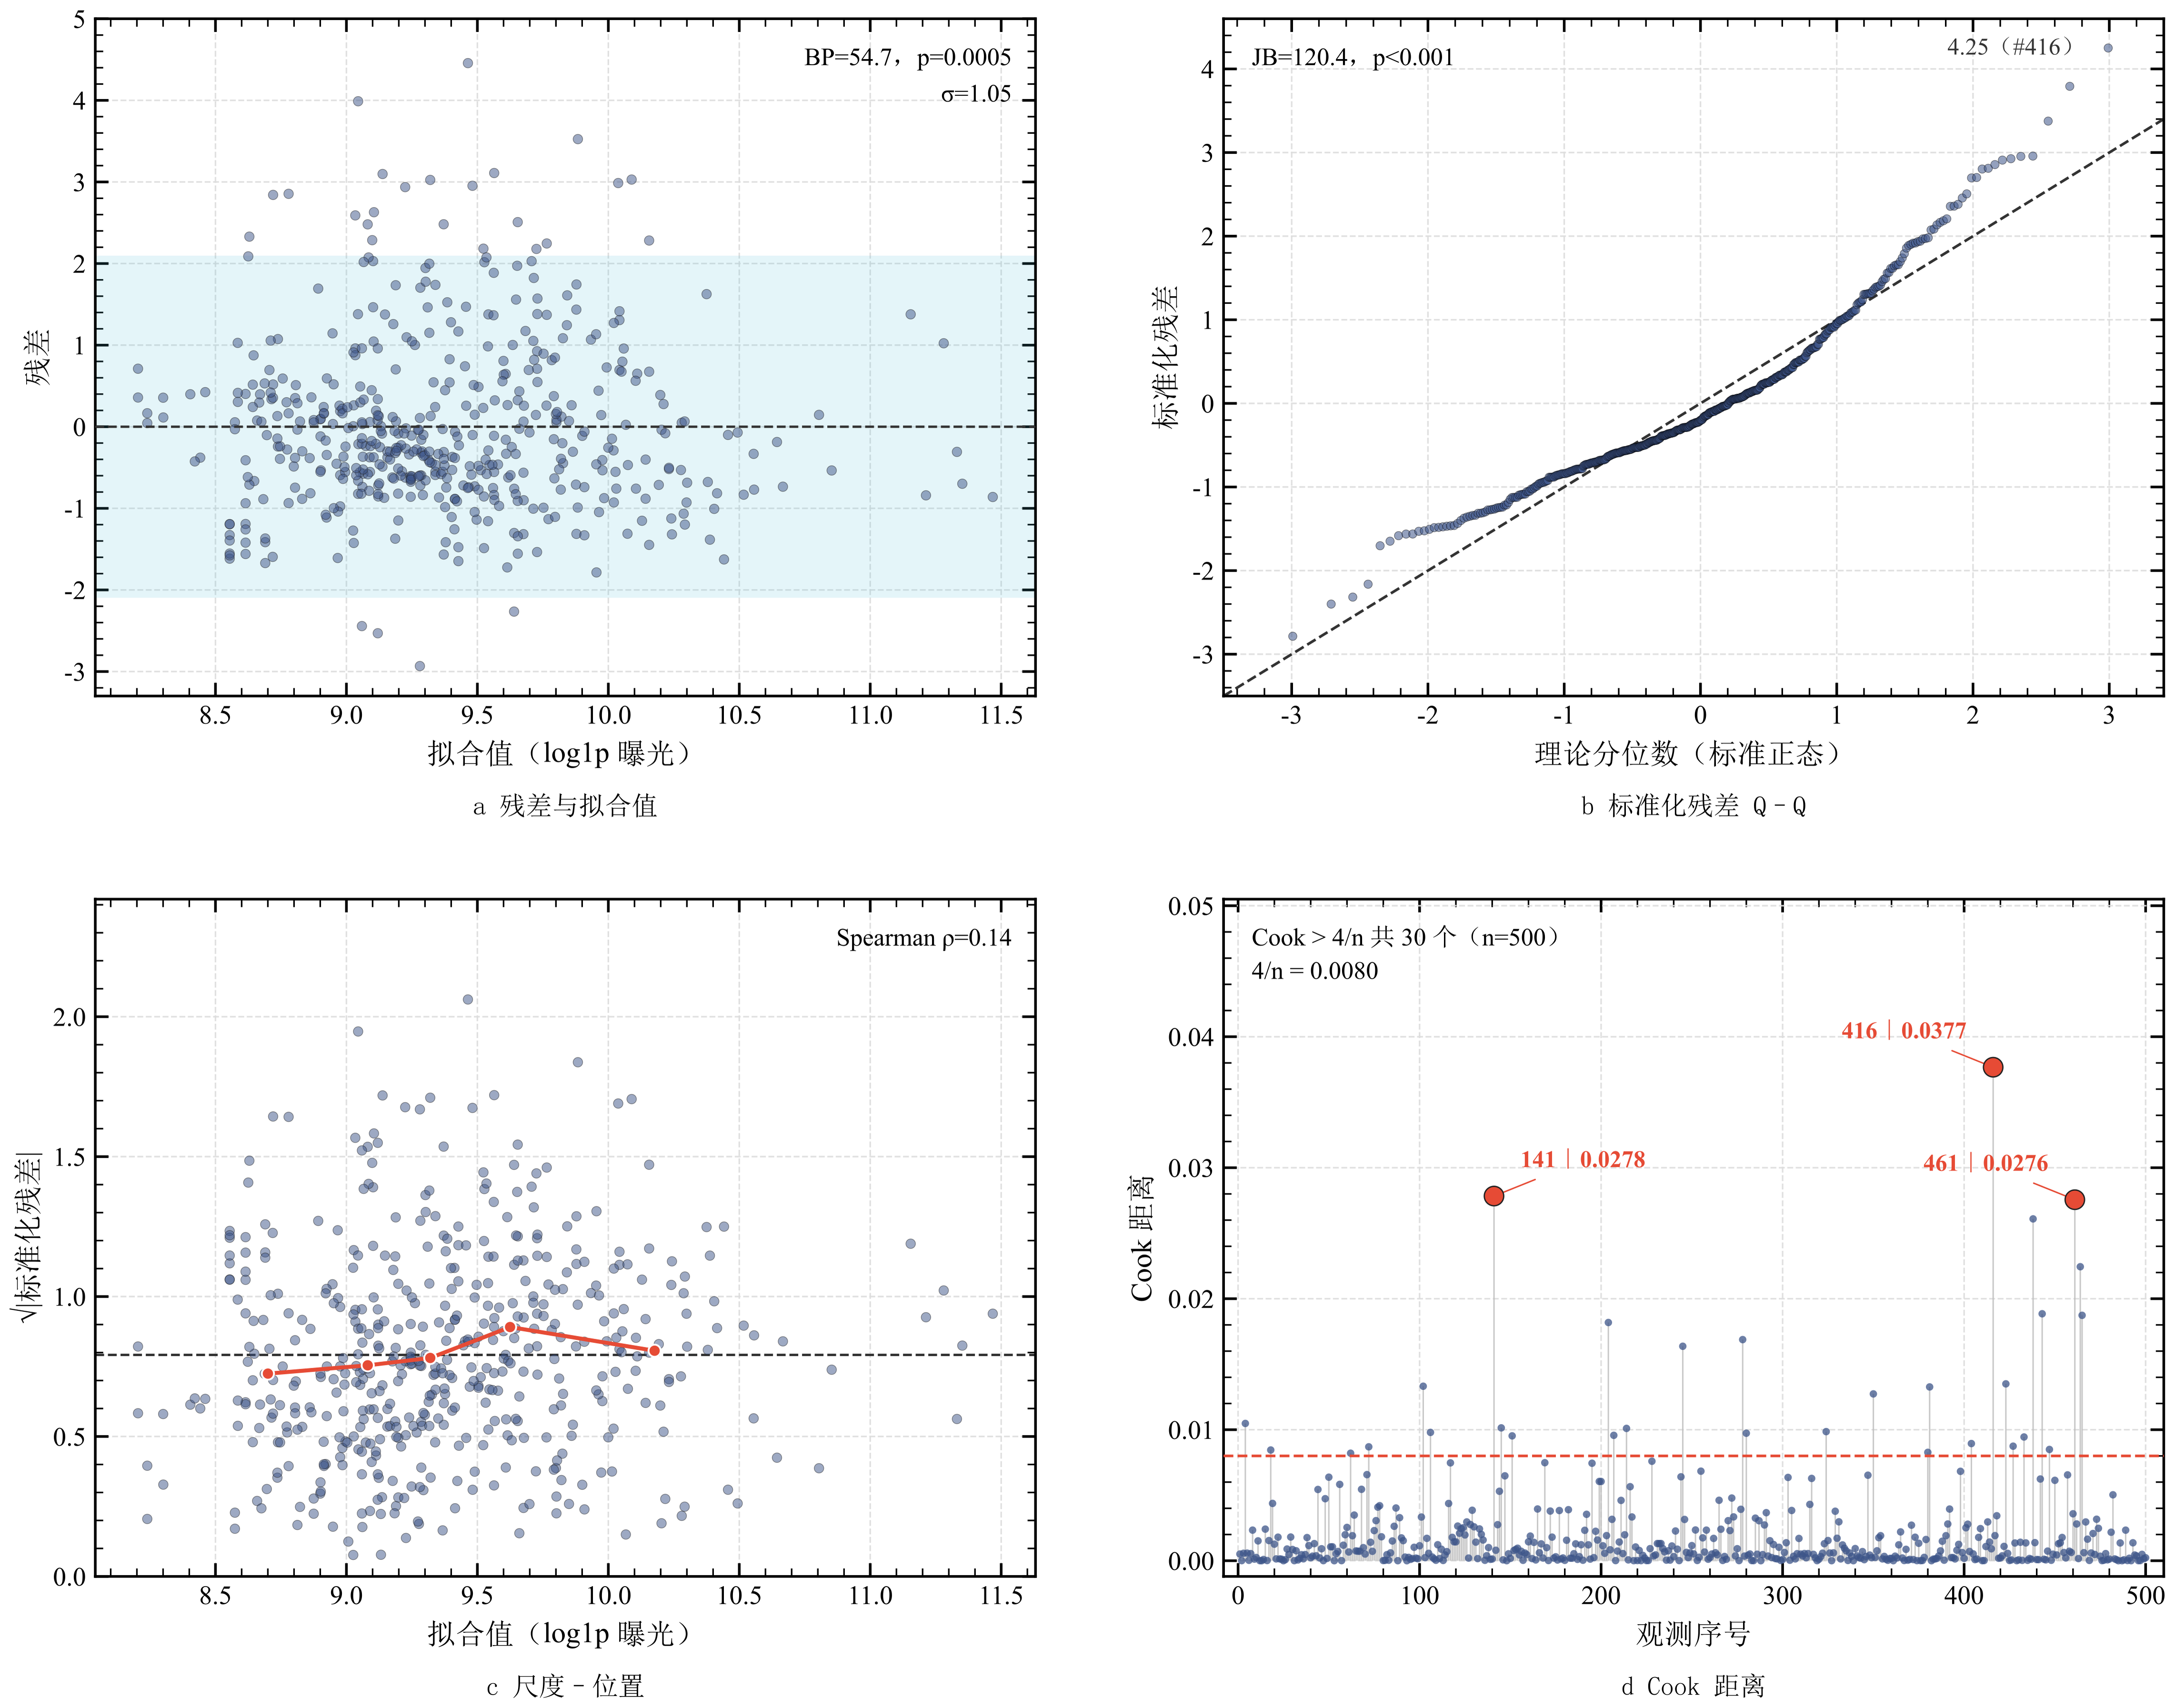
\includegraphics[width=0.68\textwidth]{../求解/问题三/结果/图8_残差诊断.png}
  \caption{最终模型残差诊断}
  \label{fig:q3_resid}
\end{figure}

图\ref{fig:q3_resid}把残差结构可视化。残差对拟合值呈水平带状分布，均值接近 0，但在低拟合值区略厚；Q--Q 图两端偏离参考线，对应少数极端曝光帖；尺度—位置图的平滑线基本水平，Spearman 相关仅 0.14，说明异方差主要来自尾部而非系统性趋势；Cook 距离图显示 30 个观测超过 $4/n$ 参考线，最高为编号 416 的 0.0377，其余依次为 141 的 0.0278 与 461 的 0.0276。整体看，残差没有呈现明显的非线性或漏斗形，HC3 标准误足以应对剩余的异方差。

\subsubsection{拟合优度与方差分解}

图\ref{fig:q3_cv}对比样本内与交叉验证表现。左图中各模型的 CV $R^2$ 都低于样本内 $R^2$，M2 由 0.2068 降至 0.1010，降幅约一半，说明模型存在一定过拟合，但方向仍为正；M1 的降幅更大，M0 的 CV $R^2$ 为 $-0.0212$。右图为 M2 的交叉验证预测与观测对照，点云沿 45 度线分布，但离散程度较大，CV $R^2$ 仅 0.101、RMSE 1.101、MAE 0.833，说明单条帖子的曝光量很难被完全预测，模型的价值在于识别平均效应而非精确点预测。

\begin{figure}[ht]
  \centering
  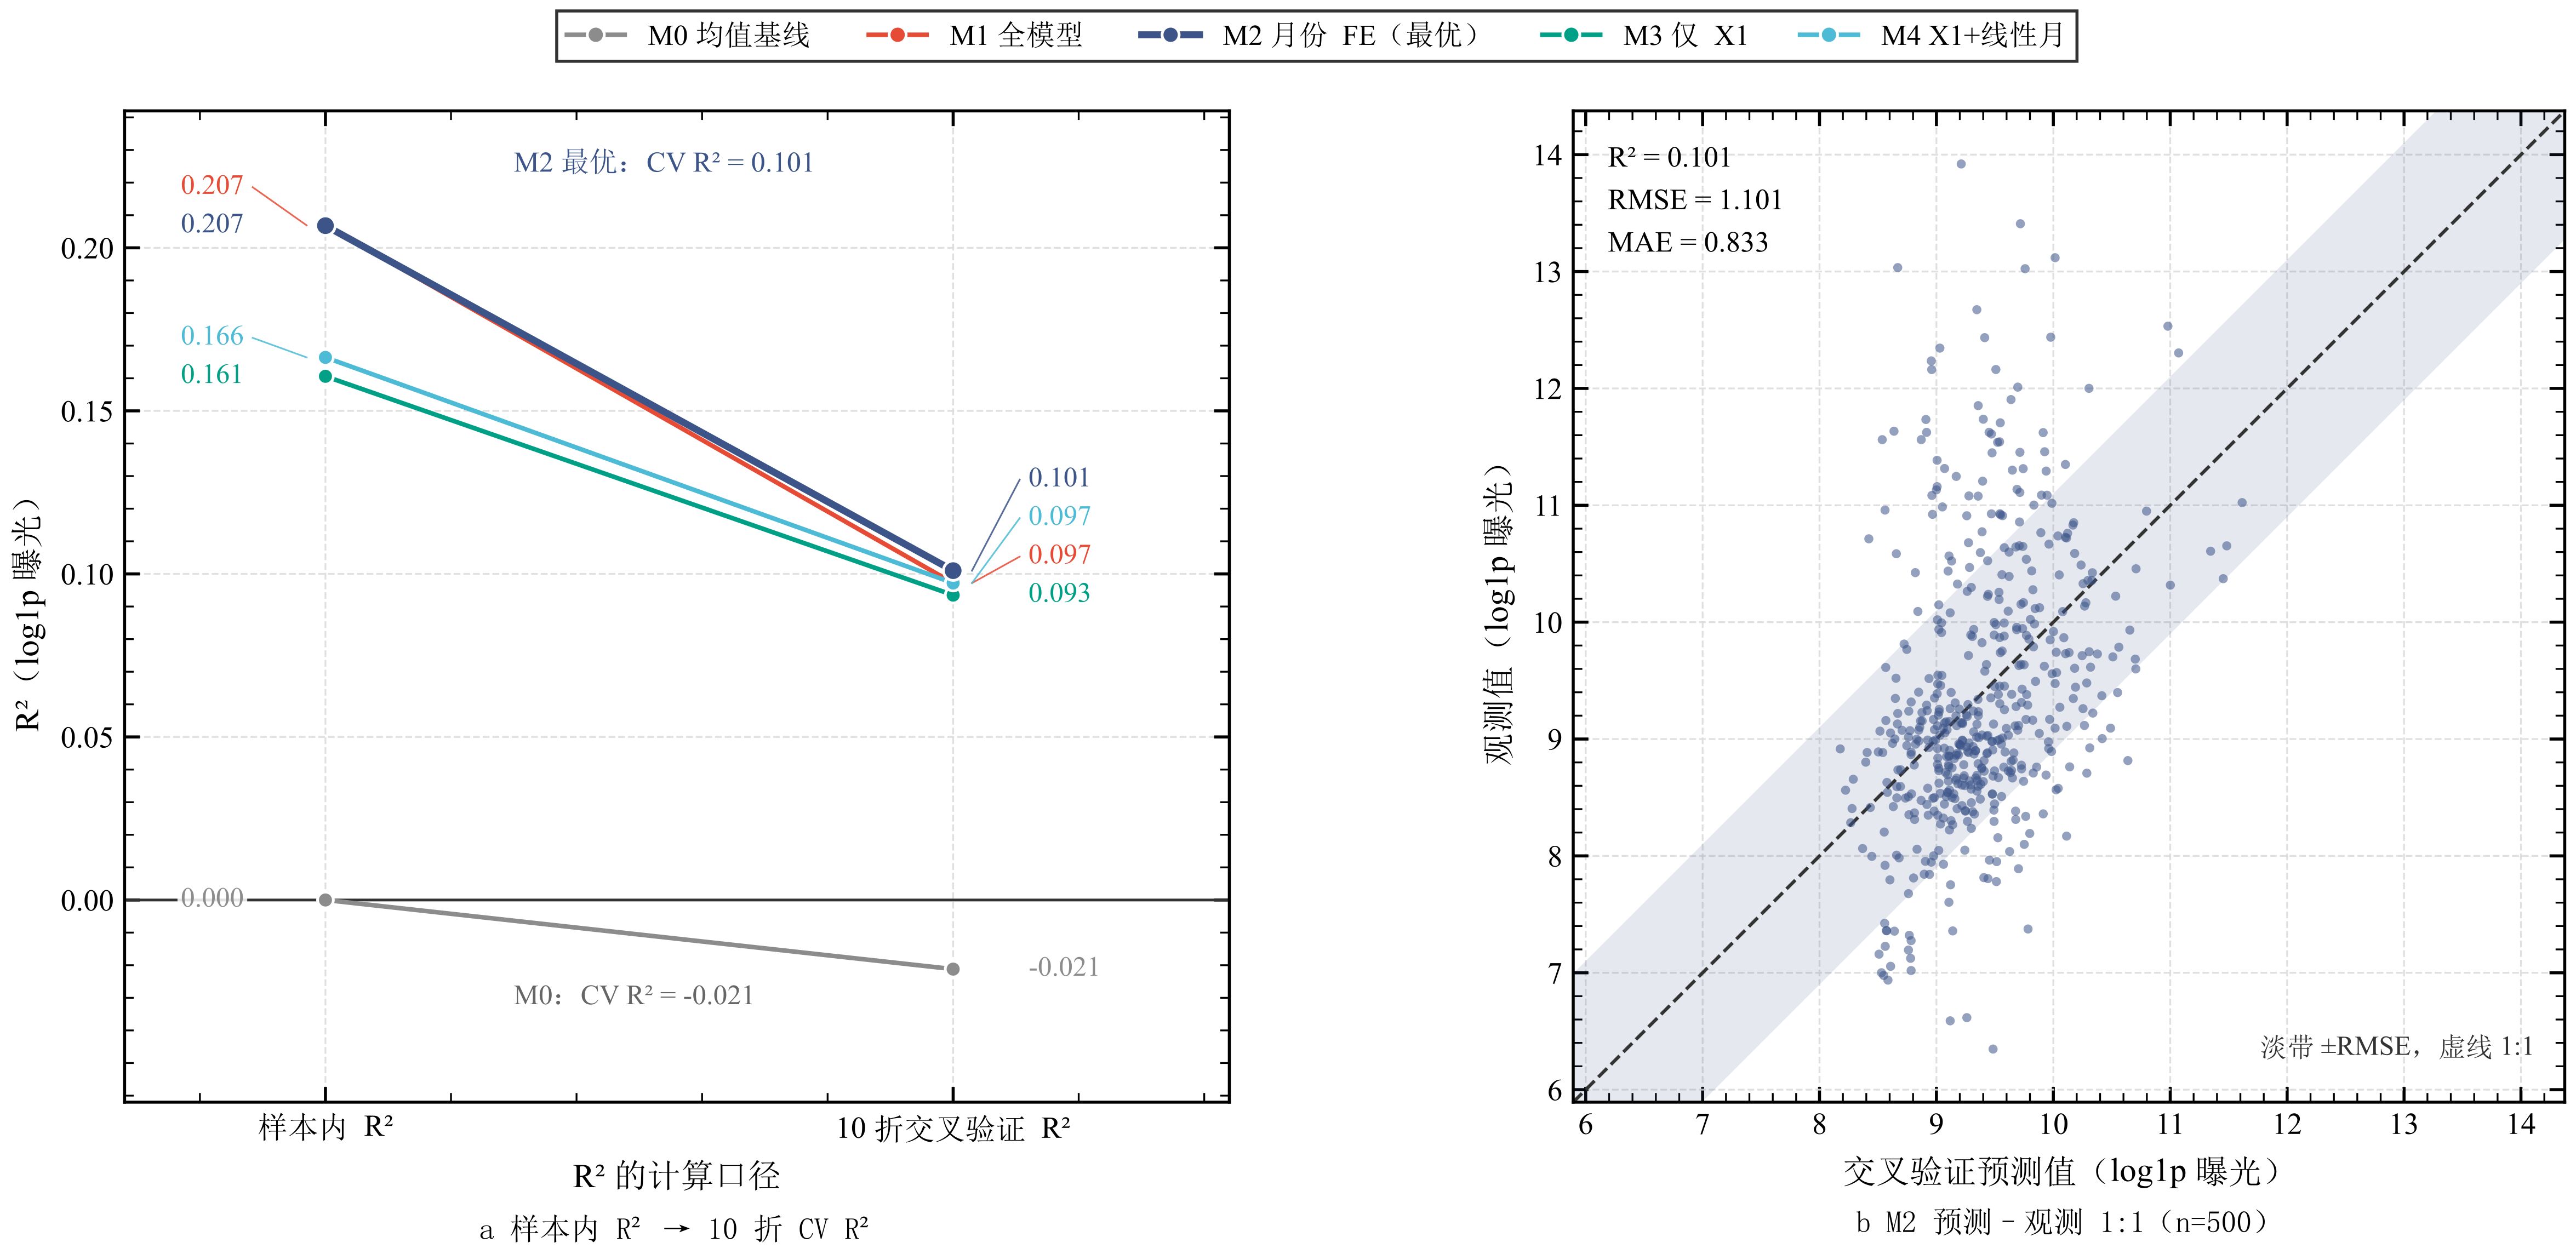
\includegraphics[width=0.74\textwidth]{../求解/问题三/结果/图9_预测能力验证.png}
  \caption{样本内与交叉验证预测能力}
  \label{fig:q3_cv}
\end{figure}

最后给出方差分解。图\ref{fig:q3_shapley}显示，帖子类型 X2 的 Shapley 贡献为 0.0767，占已解释方差的 37.1\%，是单一变量组中最大的；月份 X4 为 0.0579、占 28.0\%；付费 X7 为 0.0244、占 11.8\%；星期 X5 为 0.0236、占 11.4\%；内容主题 X3 为 0.0142、占 6.9\%；时段 X6 为 0.0055、占 2.6\%；粉丝规模 $\log X_1$ 仅为 0.0046、占 2.2\%。按类别合并，发帖决策合计解释 0.1445，占总方差的 14.45\%；账号规模与时间合计解释 0.0624，占 6.24\%；未解释部分为 0.7931，占 79.31\%。发帖决策的贡献是规模与时间的两倍以上，说明可操控的内容与投放选择比账号自然增长更能解释帖子间的曝光差异；但两者合计仍不足总方差的三分之一，绝大多数变异来自未被观测到的推荐算法、受众匹配与传播随机性。

\begin{figure}[ht]
  \centering
  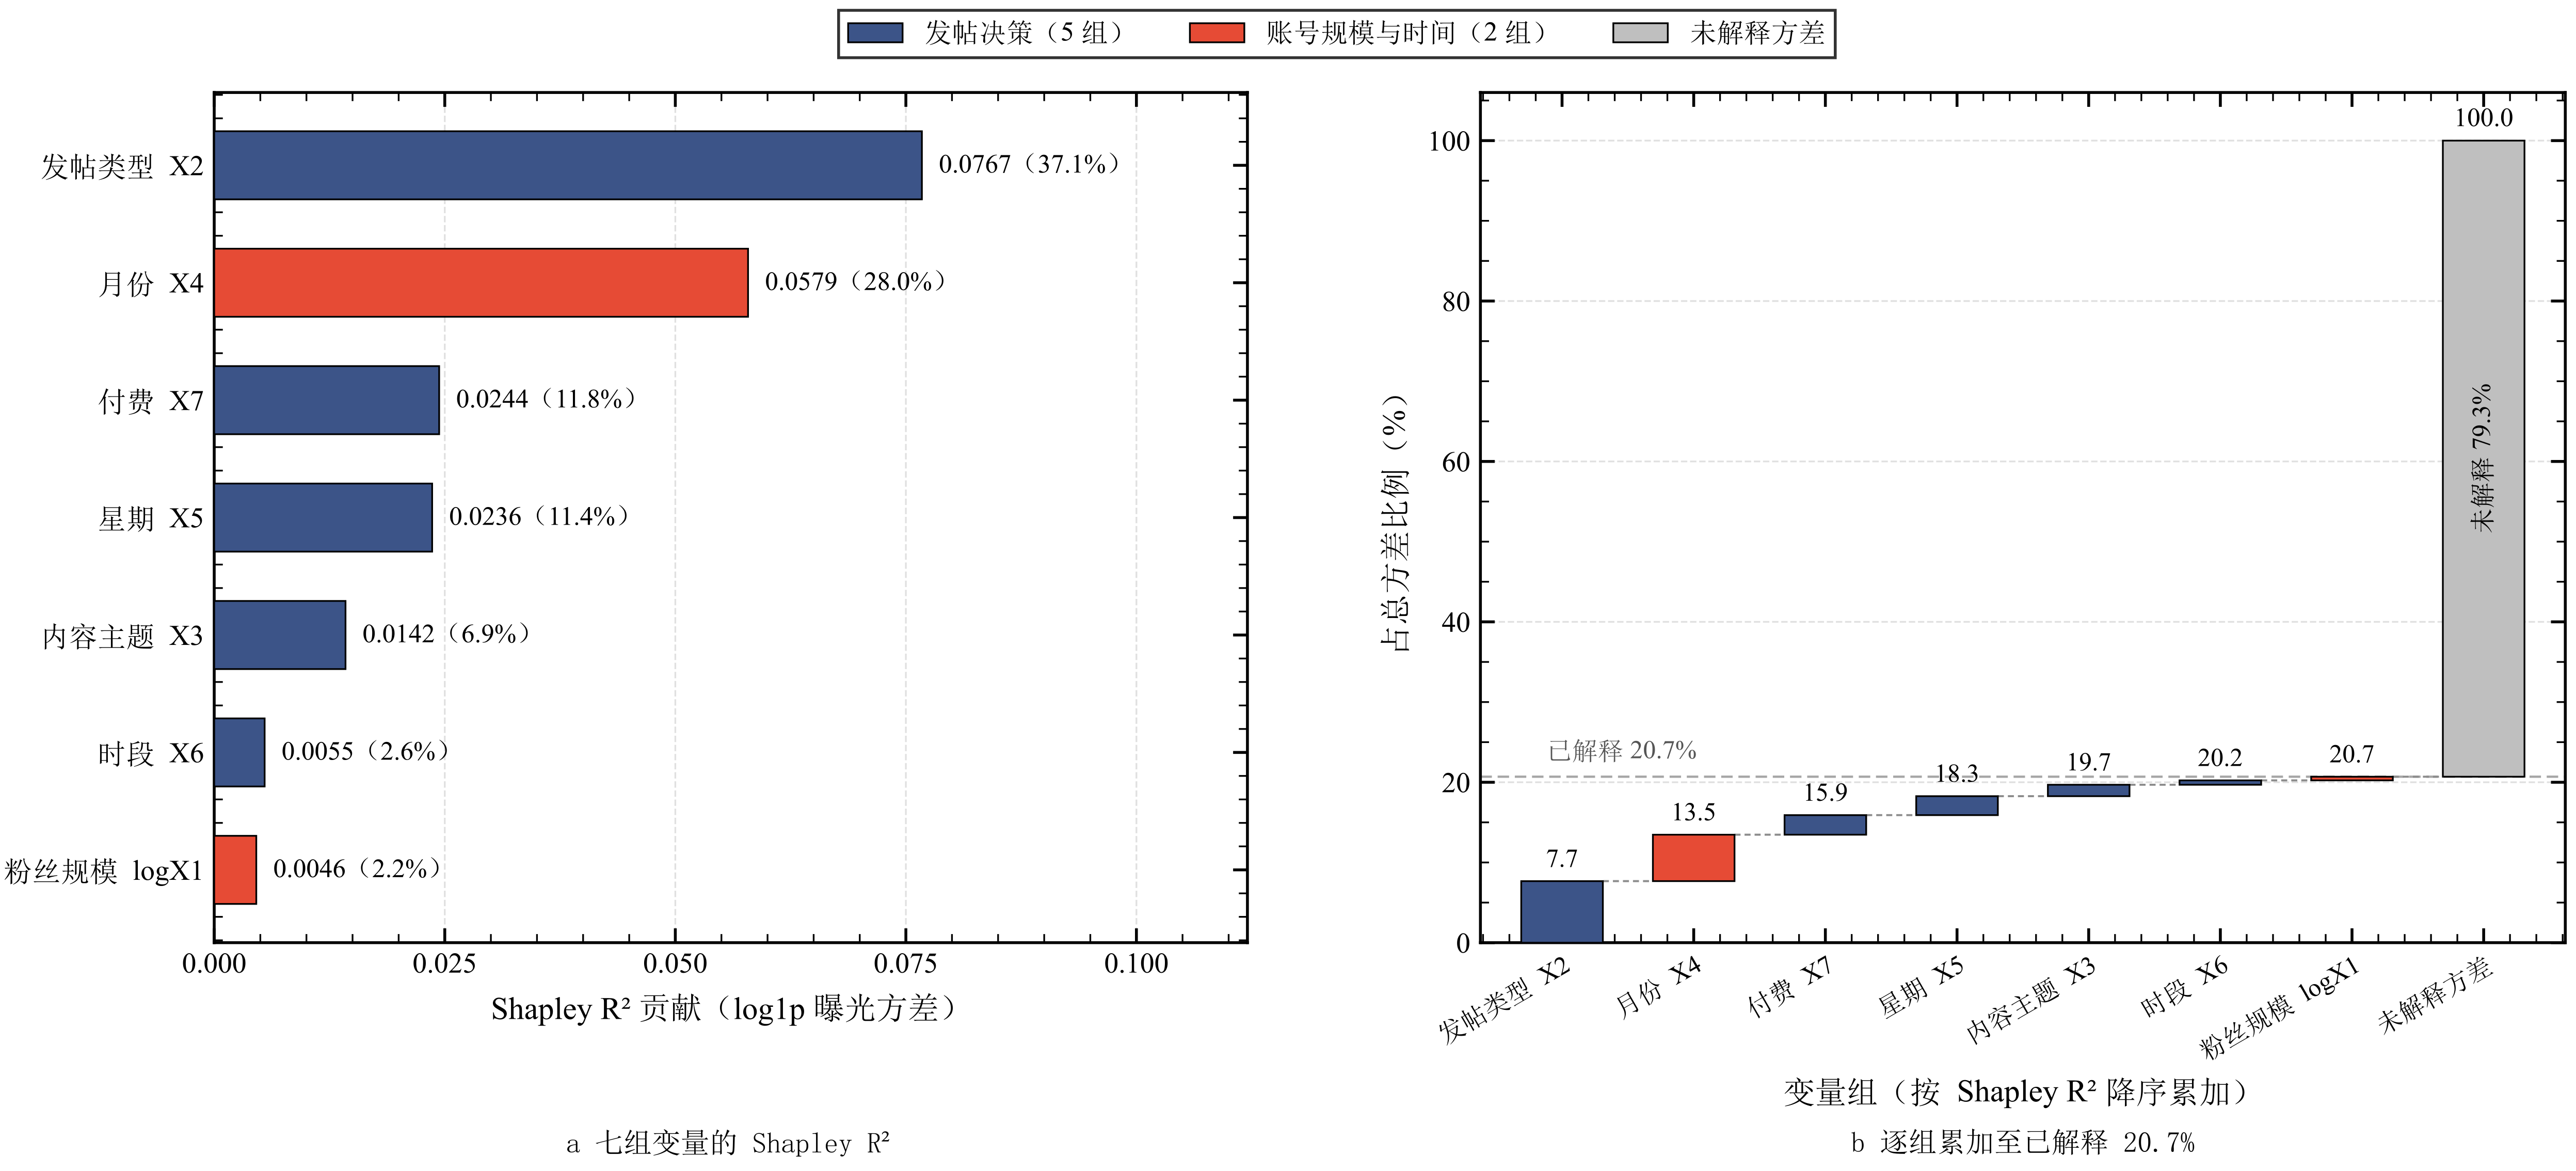
\includegraphics[width=0.74\textwidth]{../求解/问题三/结果/图10_方差贡献Shapley.png}
  \caption{变量组的 Shapley 方差贡献与总方差构成}
  \label{fig:q3_shapley}
\end{figure}

综合以上结果，M1 的粉丝规模系数在共线下不可识别，M2 以月份固定效应替代后共线消除、拟合几乎不变、交叉验证略优。最终模型在整体显著性与残差诊断上基本合格，样本外 $R^2$ 为 0.101，能够支撑平均效应测算，但不适合对单条帖子做精确点预测。发帖决策解释 14.45\% 的曝光方差，是后续效应测算的重点对象。


% ════════════════════════════════════════════
% 效应测算与决策解释（5.4）
% ════════════════════════════════════════════
\subsection{效应测算与决策解释}

\subsubsection{测算口径与可比性}

本部分读取回归阶段保存的最终模型 M2，固定一组代表性画像，使不同处理组之间只差一个变量。画像取 Photo、主题 1、7 月、周四、上午、粉丝规模 129,600 人；该组合的各个水平在样本中都有充足观测，避免外推到稀疏单元。付费情景只把付费标记改为 1，自然情景改为 0，其余分量保持不变。需要说明的是，粉丝规模与月份在样本中近乎一一对应，月份对粉丝规模对数的解释度达 0.9917，M2 以月份固定效应吸收规模趋势；因此画像中的粉丝规模取值用于标明情景所处的发展阶段，在样本的规模—月份对应关系下，固定月份、内容类型与时段后，处理组与对照组之间即满足“粉丝量相同”的口径。

最终模型的因变量为 log1p 曝光量，线性预测值只能解释为对数尺度上的条件均值。若直接取指数，得到的是条件几何均值，会系统性低估曝光次数的算术均值。Duan 提出的烟雾还原用残差的经验分布修正这一偏差\cite{duan1983}：
\begin{equation}
    \hat m(\boldsymbol{x})=e^{\hat\eta(\boldsymbol{x})}\hat\lambda-1,
    \qquad
    \hat\lambda=\frac{1}{n}\sum_{i=1}^{n}e^{e_i},
\end{equation}
其中 $\hat\eta(\boldsymbol{x})$ 为对数尺度预测值，$e_i$ 为训练样本残差，$\hat\lambda$ 为烟雾因子，本样本为 2.1896。区间估计采用参数模拟：从以点估计为均值、以 HC3 协方差为协方差矩阵的多元正态分布中独立抽取 1000 组系数，每组计算代表性画像与全样本的效应，取 2.5\% 与 97.5\% 分位数作为 95\% 区间。该方法同时传播多个系数的协方差，适合倍数与差值这类非线性函数。

在解读付费系数前，图\ref{fig:q4_balance}核对两组可比性。左上图把两组粉丝规模对数的提琴图、箱线与散点并排，自然组与付费组的均值分别为 11.711 与 11.715，标准化均值差仅 0.031，两个分布几乎完全重叠；右上图逐月给出付费占比与 Wilson 95\% 区间，各月在 16.0\% 至 40.0\% 之间波动，整体线 27.8\% 落在多数月份的区间内；左下与右下分别给出类型与主题构成，Photo 在两组都占 85\% 以上，主题构成的差异不超过 4.2 个百分点。唯一可见的差异是付费组 Video 占 2.9\%、自然组仅 0.8\%，但 Video 总共只有 7 条，且回归已用类型哑变量吸收其影响。由此可见，两组在可观测特征上接近，后文约 40\% 的提升不太可能由粉丝规模或内容构成差异解释。

\begin{figure}[ht]
  \centering
  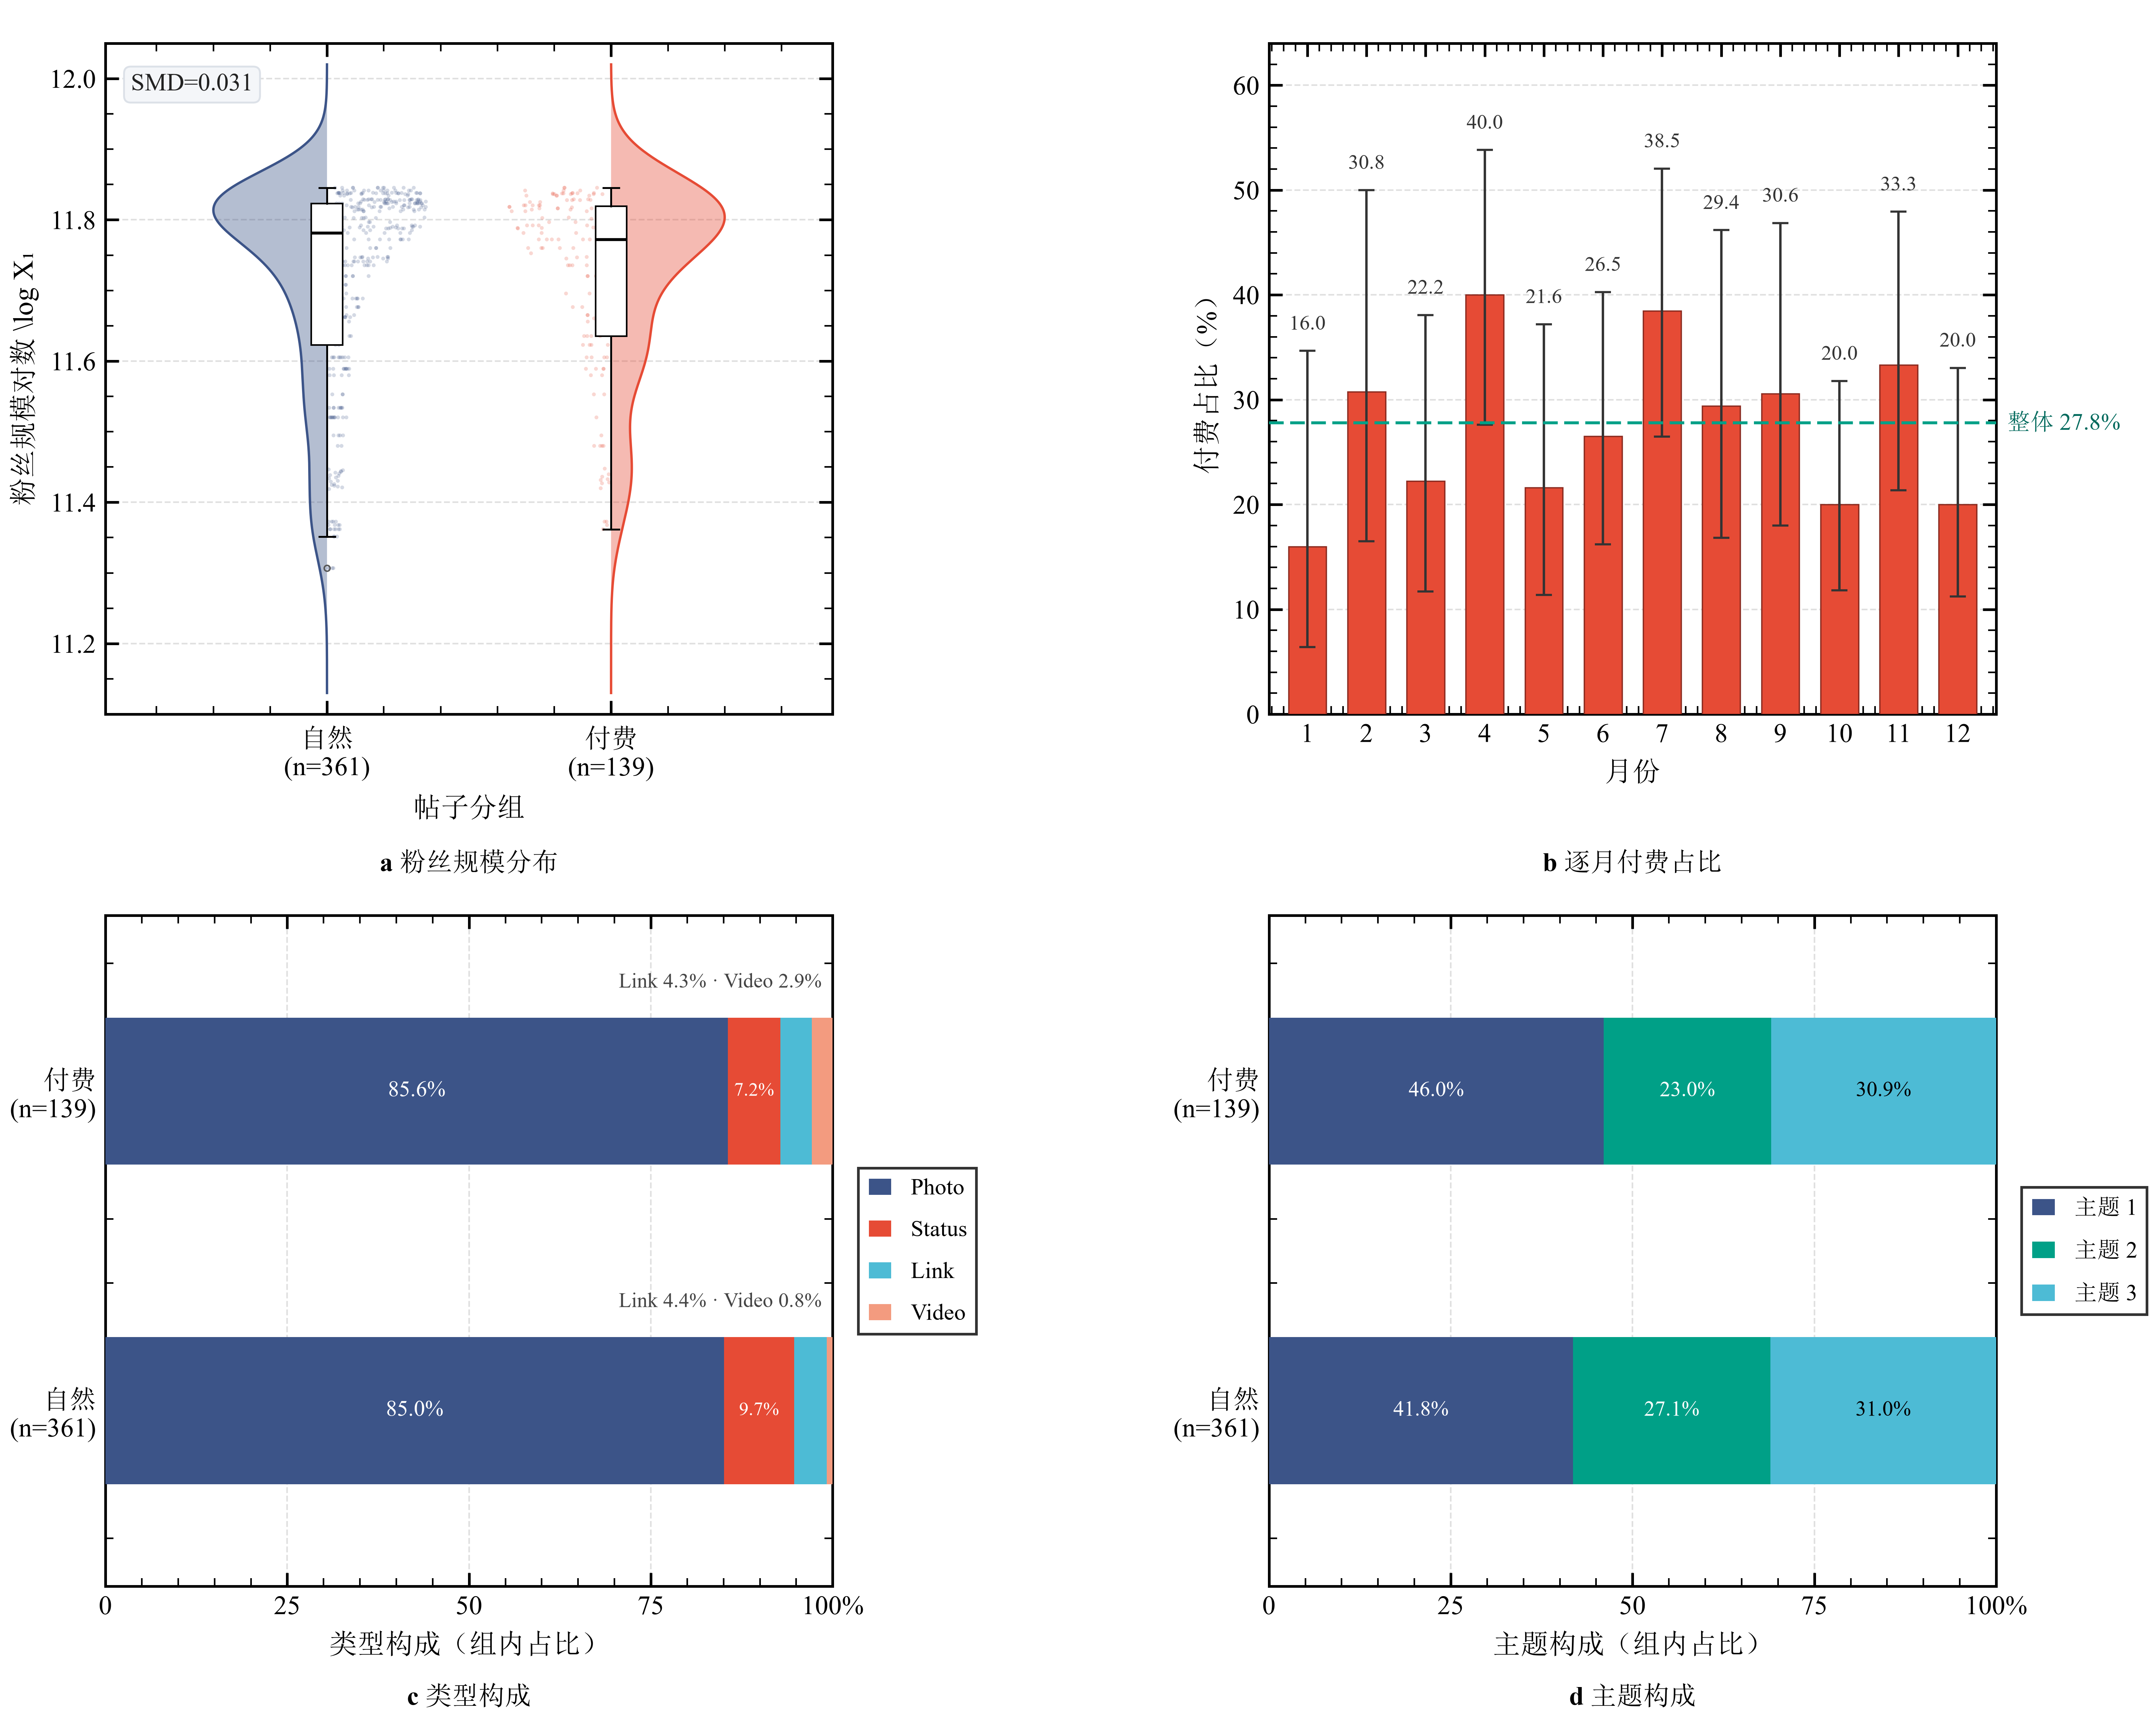
\includegraphics[width=0.70\textwidth]{../求解/临时产物/补充图3_付费可比性.png}
  \caption{付费组与自然组的可比性}
  \label{fig:q4_balance}
\end{figure}

\subsubsection{付费、类型与主题效应}

付费效应的点估计为 0.3374，HC3 标准误 0.1195，95\% 置信区间 0.1025 至 0.5723，对应净提升 40.13\%、区间 10.80\% 至 77.24\%。在代表性画像上，自然帖子的调整预测曝光为 40,221 次，付费帖子为 56,364 次，差值 16,142 次，区间 4,543 至 33,467 次，倍数 1.401、区间 1.104 至 1.753。全样本反事实的平均处理效应为 10,907 次，区间 3,138 至 20,195 次，倍数同样为 1.401。作为未调整的对照，完整案例中付费组的中位曝光为 12,060 次、自然组为 8,443 次，中位数比 1.429；填补后自然组为 361 条、中位 8,387 次，比值 1.438，与调整后的 1.401 非常接近，说明付费的正向差异不是由内容类型或发布时机的构成差异造成的。

图\ref{fig:q4_pred}把付费、类型与主题的调整预测放在同一张图中。左上图显示付费与自然的区间在曝光尺度上有重叠，但点估计的差值明确为正；右上图按类型排列，Video 的点估计远高于其他三类，区间也最宽；左下图显示主题 2 的调整预测最低（2.49 万次），主题 1 最高（4.02 万次），主题 3 为 2.94 万次；右下图按付费与类型分组给出观测中位数，Photo、Status、Link 三条连线向上，Video 因仅 7 条且付费组只有 4 条，中位数由 5.70 万次降至 5.08 万次。交互检验的 $p$ 值为 0.530，不能据此认为付费效应在不同内容类型之间存在显著差异，主效应模型已经足够。

\begin{figure}[ht]
  \centering
  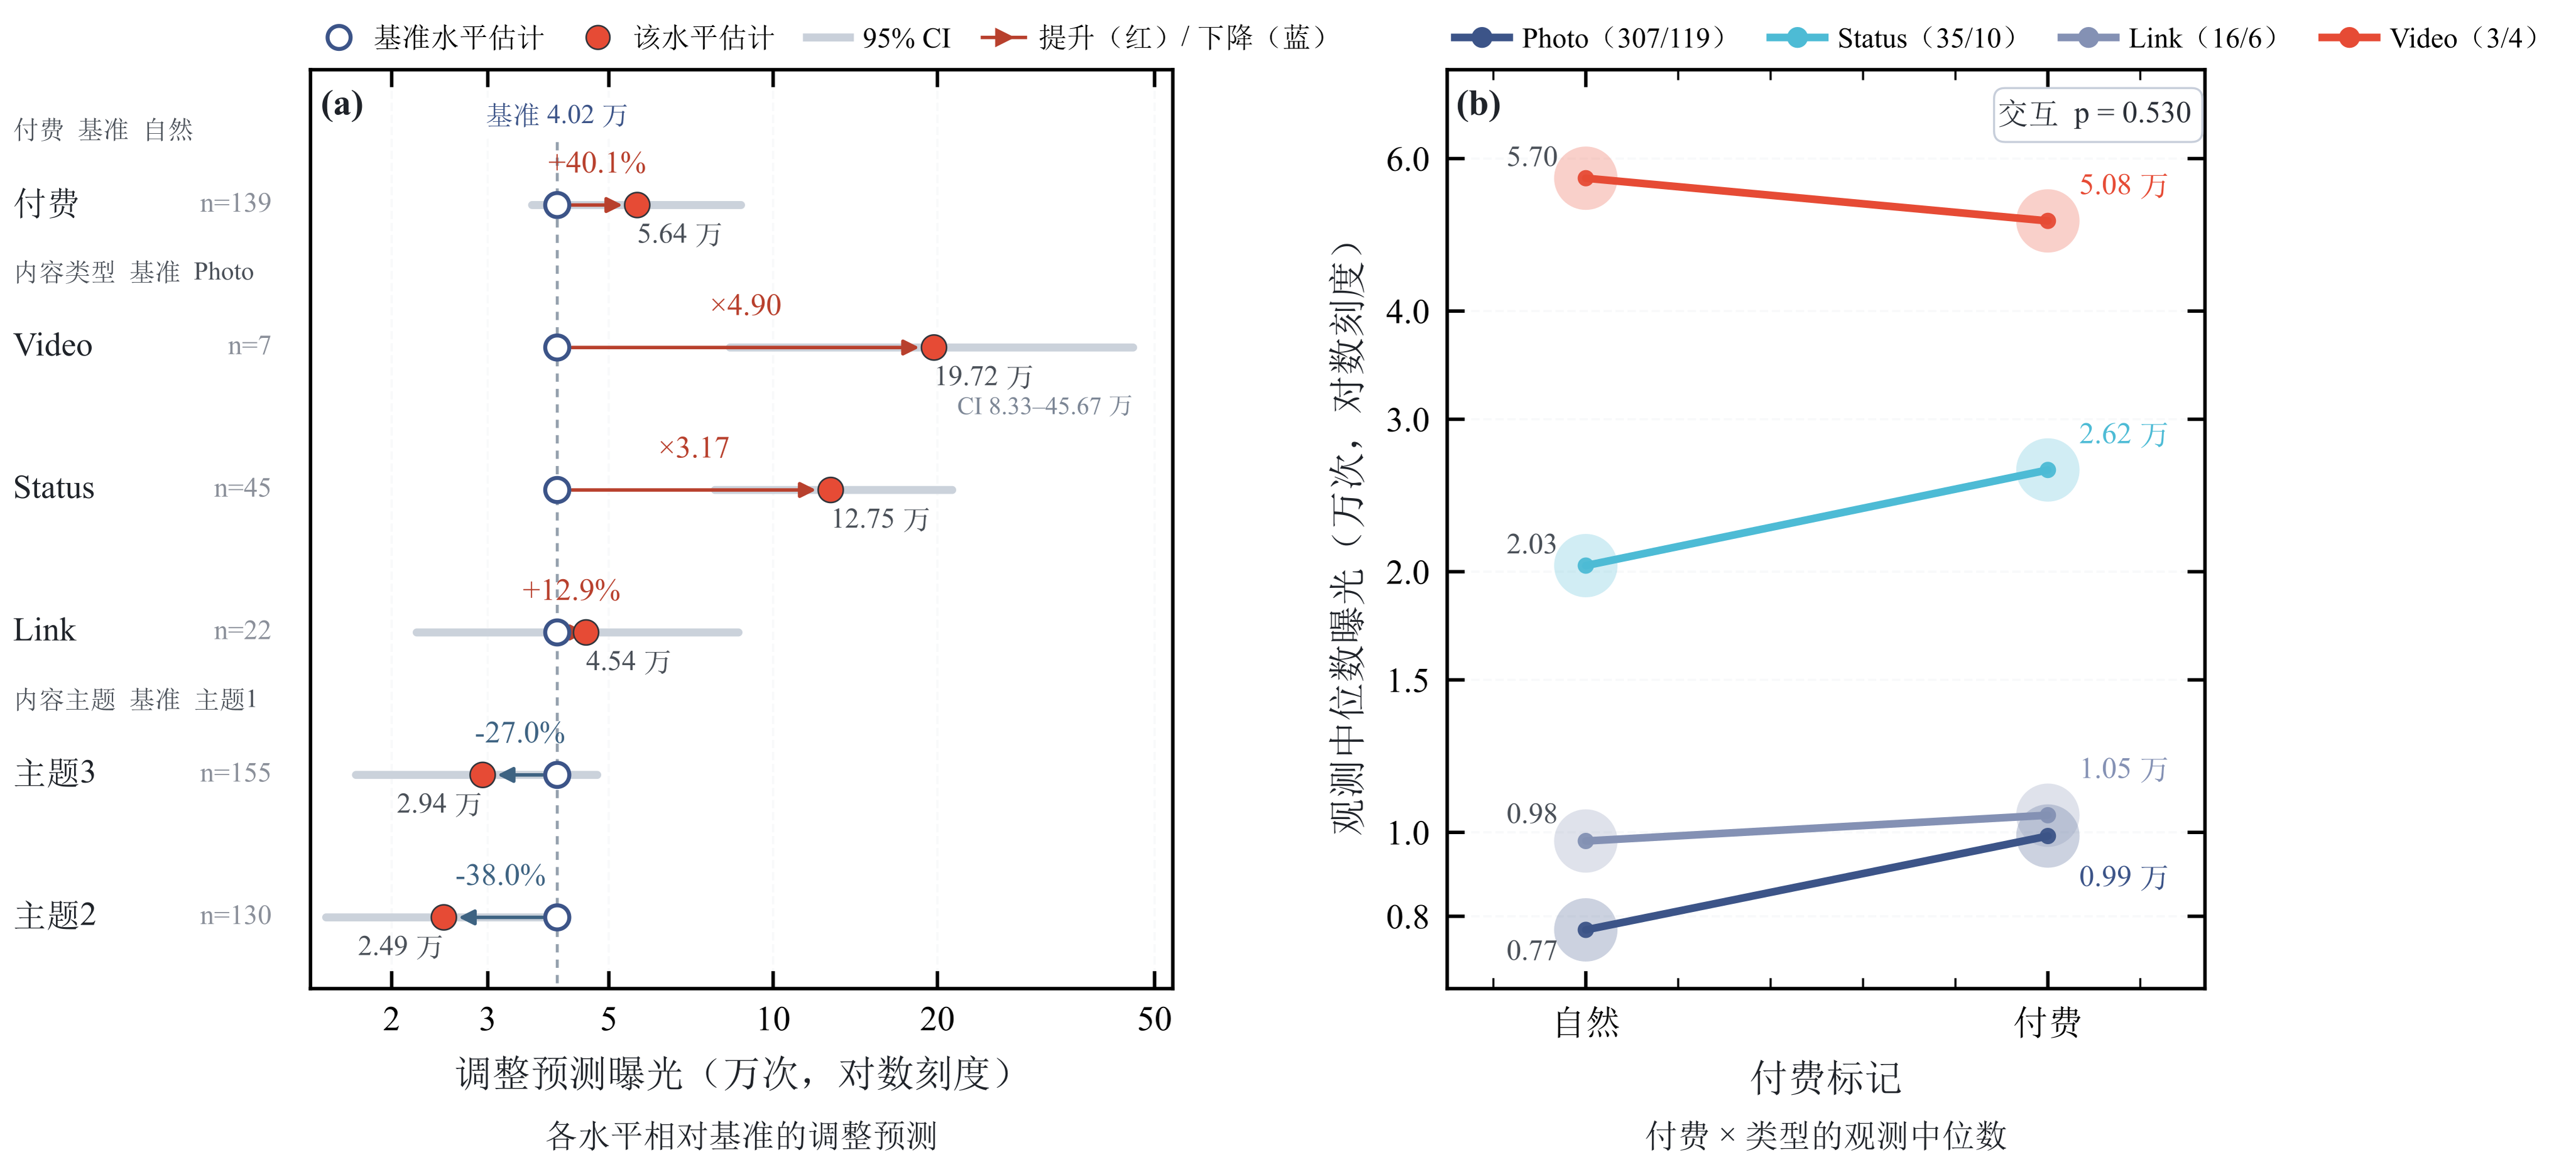
\includegraphics[width=0.75\textwidth]{../求解/问题四/结果/图11_调整预测效应.png}
  \caption{付费、内容类型与内容主题的调整预测曝光}
  \label{fig:q4_pred}
\end{figure}

内容类型与内容主题的对比如表\ref{tab:q4_effect}所示。以 Photo 为参照，Video 的系数为 1.5896、$p$ 值 0.0001，折算为 4.90 倍，区间 2.23 至 10.79；Status 的系数为 1.1538、$p$ 值小于 0.001，折算为 3.17 倍，区间 2.49 至 4.04；Link 的系数为 0.1215、$p$ 值 0.643，折算为 1.13 倍，区间 0.68 至 1.89，与 Photo 无显著差异。在代表性画像上，Video 的调整预测曝光为 197,157 次，比 Photo 的 40,221 次多出约 15.7 万次；Status 为 127,511 次，Link 为 45,420 次。Video 的倍数最高，但其区间上限约为下限的 4.8 倍，且样本只有 7 条，解读时应把它理解为“方向明确、幅度不确定”的信号，而不是精确的投放回报。

内容主题的联合与两两结果同样列在表\ref{tab:q4_effect}。联合 Wald 统计量为 12.6783、自由度 2、$p$ 值 0.0018，拒绝“两个主题哑变量同时为零”的原假设，说明主题整体对曝光有显著影响。相对主题 1，主题 2 的系数为 $-0.4784$、折算 0.620 倍，区间 0.475 至 0.808；主题 3 的系数为 $-0.3147$、折算 0.730 倍，区间 0.561 至 0.950。两者都显著低于主题 1，且主题 2 的点估计更低。但主题 2 与主题 3 的直接差异为 $-0.1638$、$p$ 值 0.186、倍数 0.849，区间 0.666 至 1.082，在 5\% 水平不显著，不能据此断言主题 2 一定劣于主题 3。

\begin{longtable}{>{\centering\arraybackslash}p{0.19\textwidth}>{\centering\arraybackslash}p{0.085\textwidth}>{\centering\arraybackslash}p{0.085\textwidth}>{\centering\arraybackslash}p{0.08\textwidth}>{\centering\arraybackslash}p{0.07\textwidth}>{\centering\arraybackslash}p{0.07\textwidth}>{\centering\arraybackslash}p{0.07\textwidth}>{\centering\arraybackslash}p{0.07\textwidth}}
  \caption{内容类型与内容主题效应}
  \label{tab:q4_effect} \\
  \toprule
  对比 & 系数或\newline 统计量 & 标准误 & $p$ 值 & 倍数 & 倍数\newline 下限 & 倍数\newline 上限 & 处理组\newline 曝光 \\
  \midrule
  \endfirsthead
  \caption{内容类型与内容主题效应（续）} \\
  \toprule
  对比 & 系数或\newline 统计量 & 标准误 & $p$ 值 & 倍数 & 倍数\newline 下限 & 倍数\newline 上限 & 处理组\newline 曝光 \\
  \midrule
  \endhead
  \bottomrule
  \endfoot
  Video 对 Photo & 1.590 & 0.402 & 0.0001 & 4.902 & 2.226 & 10.793 & 197,157 \\
  Status 对 Photo & 1.154 & 0.124 & $<$0.001 & 3.170 & 2.487 & 4.041 & 127,511 \\
  Link 对 Photo & 0.122 & 0.262 & 0.643 & 1.129 & 0.675 & 1.889 & 45,420 \\
  主题联合 Wald & 12.678 & — & 0.0018 & — & — & — & — \\
  主题 2 对主题 1 & $-0.478$ & 0.135 & $<$0.001 & 0.620 & 0.475 & 0.808 & 24,927 \\
  主题 3 对主题 1 & $-0.315$ & 0.134 & 0.019 & 0.730 & 0.561 & 0.950 & 29,363 \\
  主题 2 对主题 3 & $-0.164$ & 0.124 & 0.186 & 0.849 & 0.666 & 1.082 & — \\
\end{longtable}

\subsubsection{稳健性与异质性}

表\ref{tab:q4_robust}汇总六种设定下的付费与视频效应。付费提升在 M1 至 M4 中为 40.09\% 至 49.65\%，Huber 回归为 37.44\%，Gamma 模型为 44.84\%，全部在 1\% 水平显著；Video 倍数在 3.52 至 5.41 之间，同样全部显著。M3 与 M4 因未使用月份固定效应，付费系数略高，说明月份控制吸收了一部分与付费相关的季节差异；Gamma 模型的 Video 倍数最低，反映其对右偏分布的拟合更保守。六种设定的方向一致、区间都不跨过 0 或 1，可以认为结论不依赖单一模型设定。

\begin{longtable}{>{\centering\arraybackslash}p{0.19\textwidth}>{\centering\arraybackslash}p{0.10\textwidth}>{\centering\arraybackslash}p{0.09\textwidth}>{\centering\arraybackslash}p{0.10\textwidth}>{\centering\arraybackslash}p{0.10\textwidth}>{\centering\arraybackslash}p{0.09\textwidth}>{\centering\arraybackslash}p{0.09\textwidth}}
  \caption{六种设定下的付费与视频效应}
  \label{tab:q4_robust} \\
  \toprule
  设定 & 付费系数 & 付费 $p$ 值 & 付费提升\newline （\%） & Video\newline 系数 & Video\newline $p$ 值 & Video\newline 倍数 \\
  \midrule
  \endfirsthead
  \caption{六种设定下的付费与视频效应（续）} \\
  \toprule
  设定 & 付费系数 & 付费 $p$ 值 & 付费提升\newline （\%） & Video\newline 系数 & Video\newline $p$ 值 & Video\newline 倍数 \\
  \midrule
  \endhead
  \bottomrule
  \endfoot
  M1 全模型 & 0.337 & 0.005 & 40.09 & 1.588 & $<$0.001 & 4.894 \\
  M2 月份固定效应 & 0.337 & 0.005 & 40.13 & 1.590 & $<$0.001 & 4.902 \\
  M3 仅 $\log X_1$ & 0.403 & 0.001 & 49.65 & 1.658 & $<$0.001 & 5.250 \\
  M4 线性月份 & 0.386 & 0.002 & 47.14 & 1.688 & $<$0.001 & 5.408 \\
  Huber 稳健回归 & 0.318 & 0.001 & 37.44 & 1.683 & $<$0.001 & 5.384 \\
  Gamma 广义线性模型 & 0.371 & 0.010 & 44.84 & 1.258 & 0.001 & 3.518 \\
\end{longtable}

\begin{figure}[ht]
  \centering
  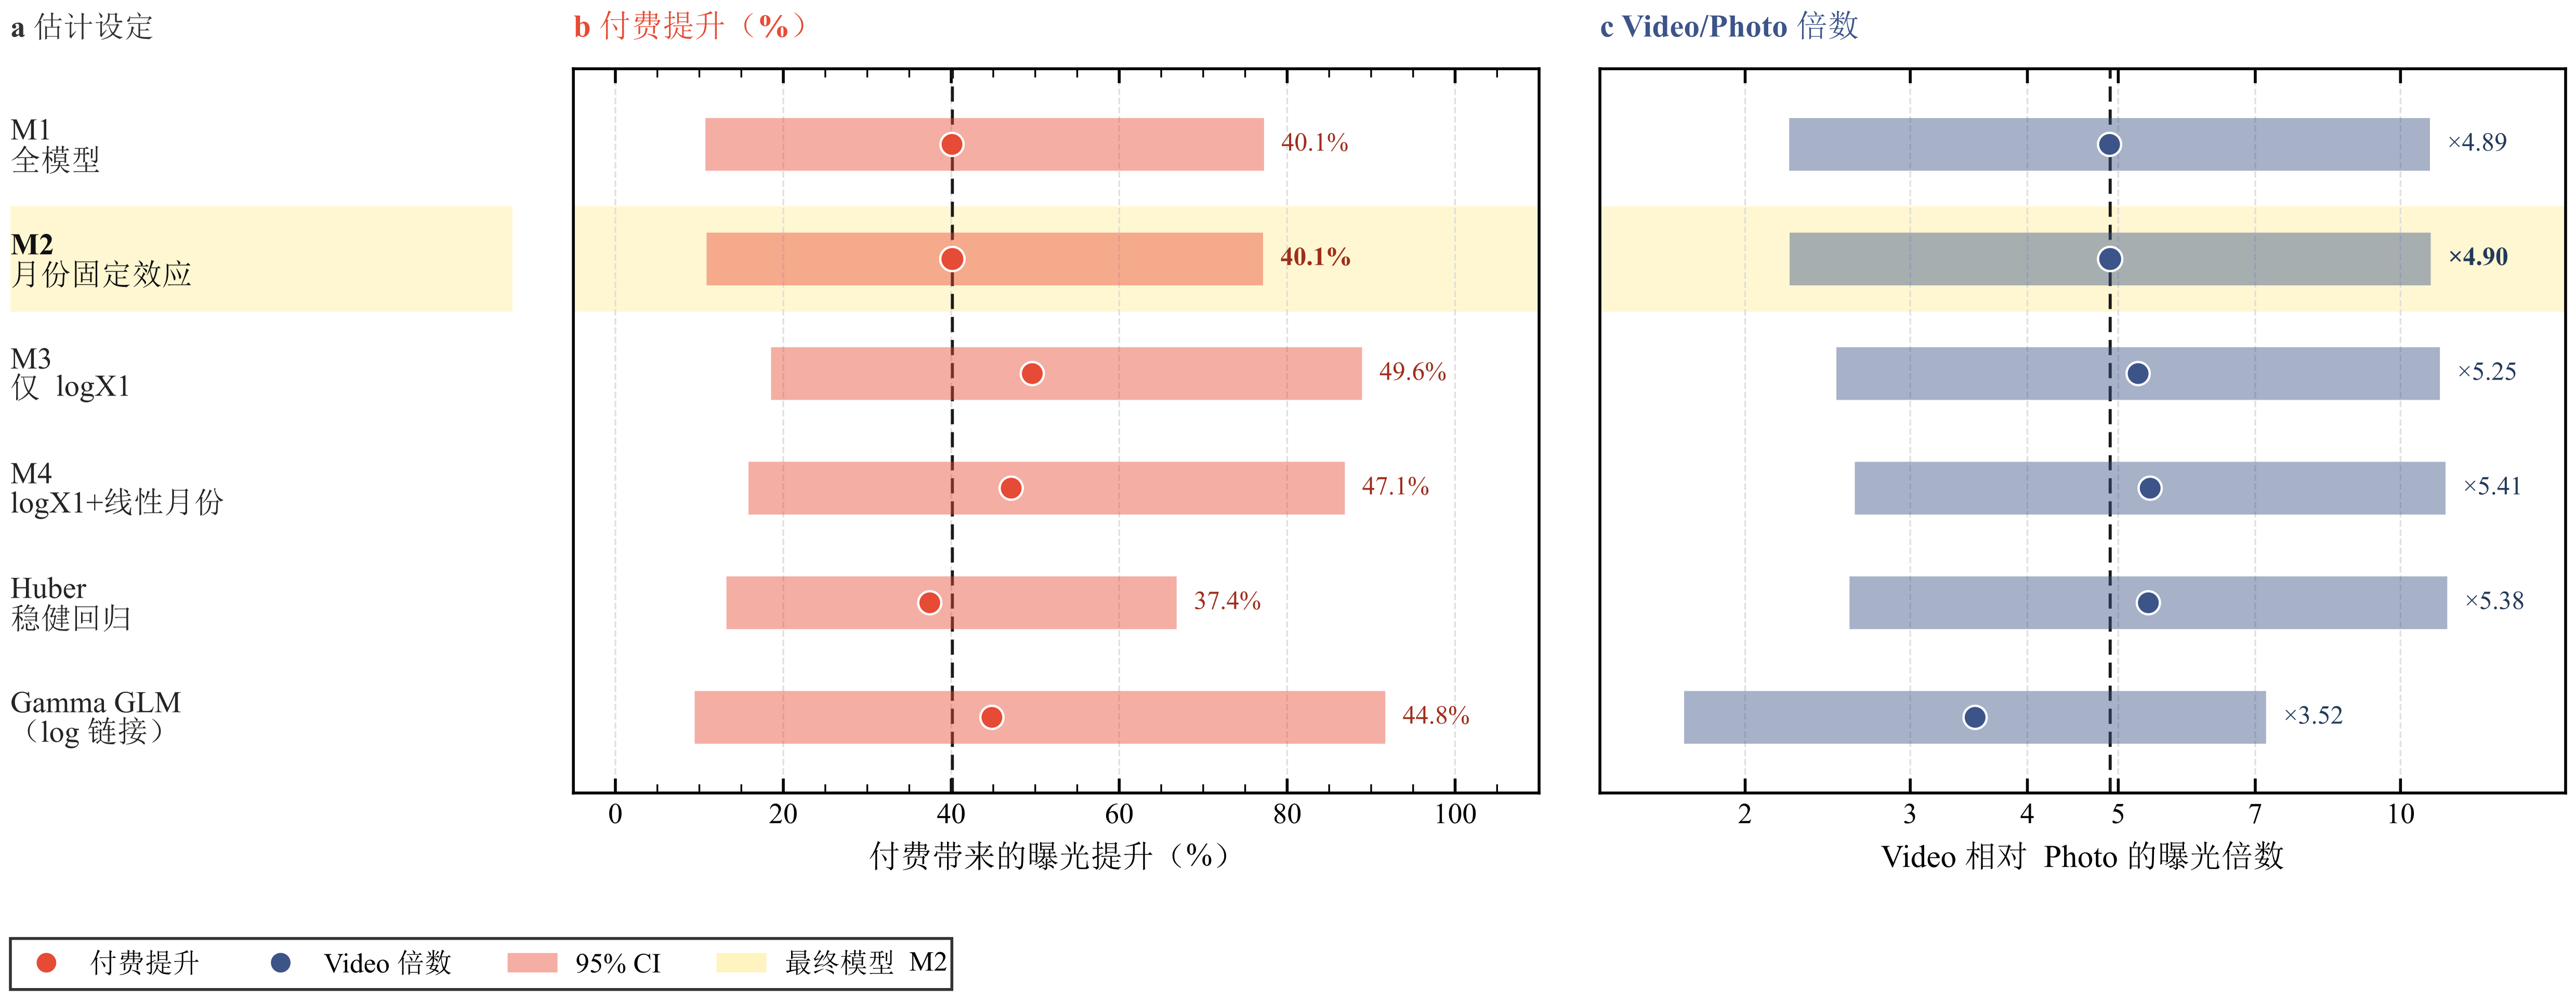
\includegraphics[width=0.75\textwidth]{../求解/问题四/结果/图12_效应稳健性.png}
  \caption{付费与视频效应在六种设定下的稳健性}
  \label{fig:q4_robust}
\end{figure}

图\ref{fig:q4_matrix}进一步把 7 个主效应在 6 种设定下的系数画成矩阵，按行归一化着色并标注显著性。付费、Video、Status、主题 2、主题 3 与时段凌晨的方向在所有设定下一致；Link 在所有设定下都不显著，Gamma 模型中甚至反号，因此不能把 Link 的相对曝光差异当作稳定结论。矩阵还显示，主题 2 的负向系数在 Gamma 模型中最强（$-0.848$），主题 3 在 M3 中减弱为不显著（$-0.236$），说明主题效应的大小对分布假设有一定敏感，但方向没有反转。

\begin{figure}[ht]
  \centering
  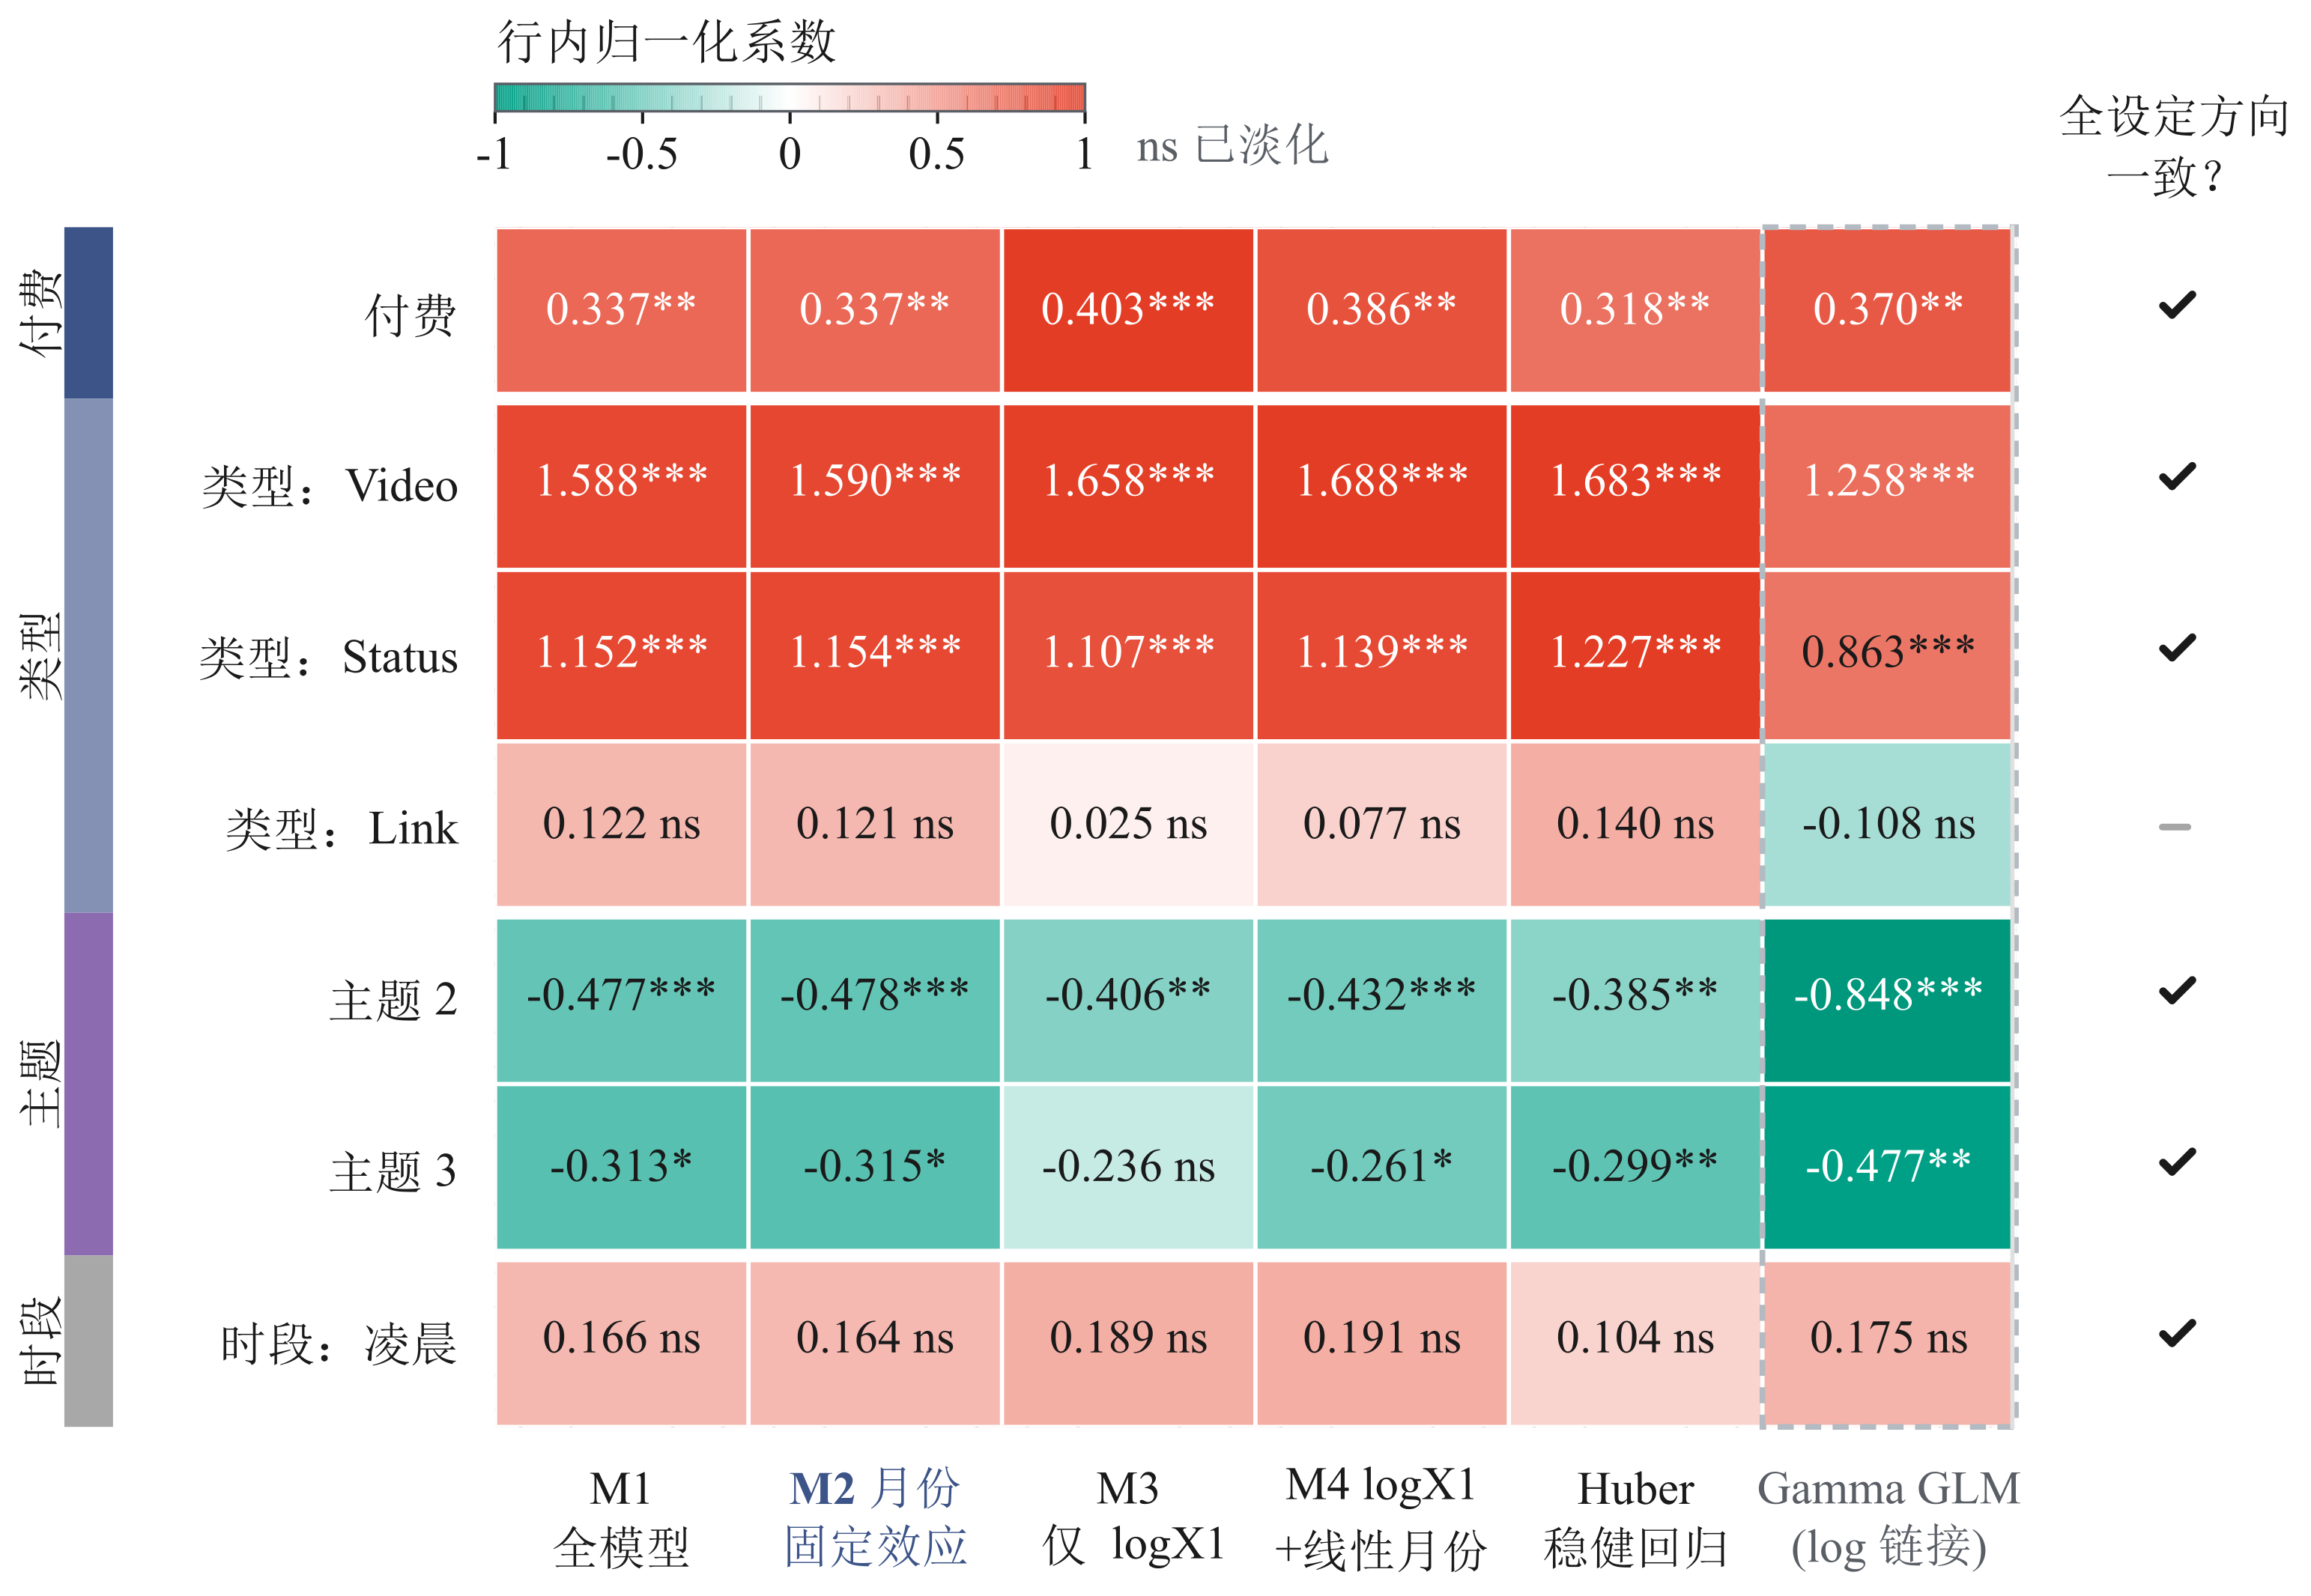
\includegraphics[width=0.70\textwidth]{../求解/问题四/结果/图16_系数稳健性矩阵.png}
  \caption{七个主效应在六种设定下的系数稳健性矩阵}
  \label{fig:q4_matrix}
\end{figure}

最后检验付费效应是否随内容特征变化。图\ref{fig:q4_het}按全样本、帖子类型、内容主题与发布时段分组，报告各组内的付费系数与交互联合检验的 $P$ 值。类型组的组内 $P$ 为 0.531，时段组为 0.474，均未拒绝“付费效应不随该维度变化”的原假设；主题组的组内 $P$ 为 0.036，在 5\% 水平显著。具体看，主题 1 的付费系数为 0.57（95\% 区间 0.15 至 0.99，$p=0.008$），主题 2 为 0.43（区间 $-0.01$ 至 0.86，$p=0.056$），主题 3 仅为 0.02（区间 $-0.40$ 至 0.45，$p=0.911$）。这说明付费投放的增量主要集中在主题 1，主题 2 处于边缘显著，主题 3 几乎看不到付费效果。若改用互斥子样本的系数 $Q$ 检验，主题组 $p$ 值为 0.172，说明该异质性证据对检验口径有一定敏感性；本报告以与图\ref{fig:q4_pred}同口径的交互联合检验为主，把主题异质性作为定向投放的参考，而不是强因果结论。

\begin{figure}[ht]
  \centering
  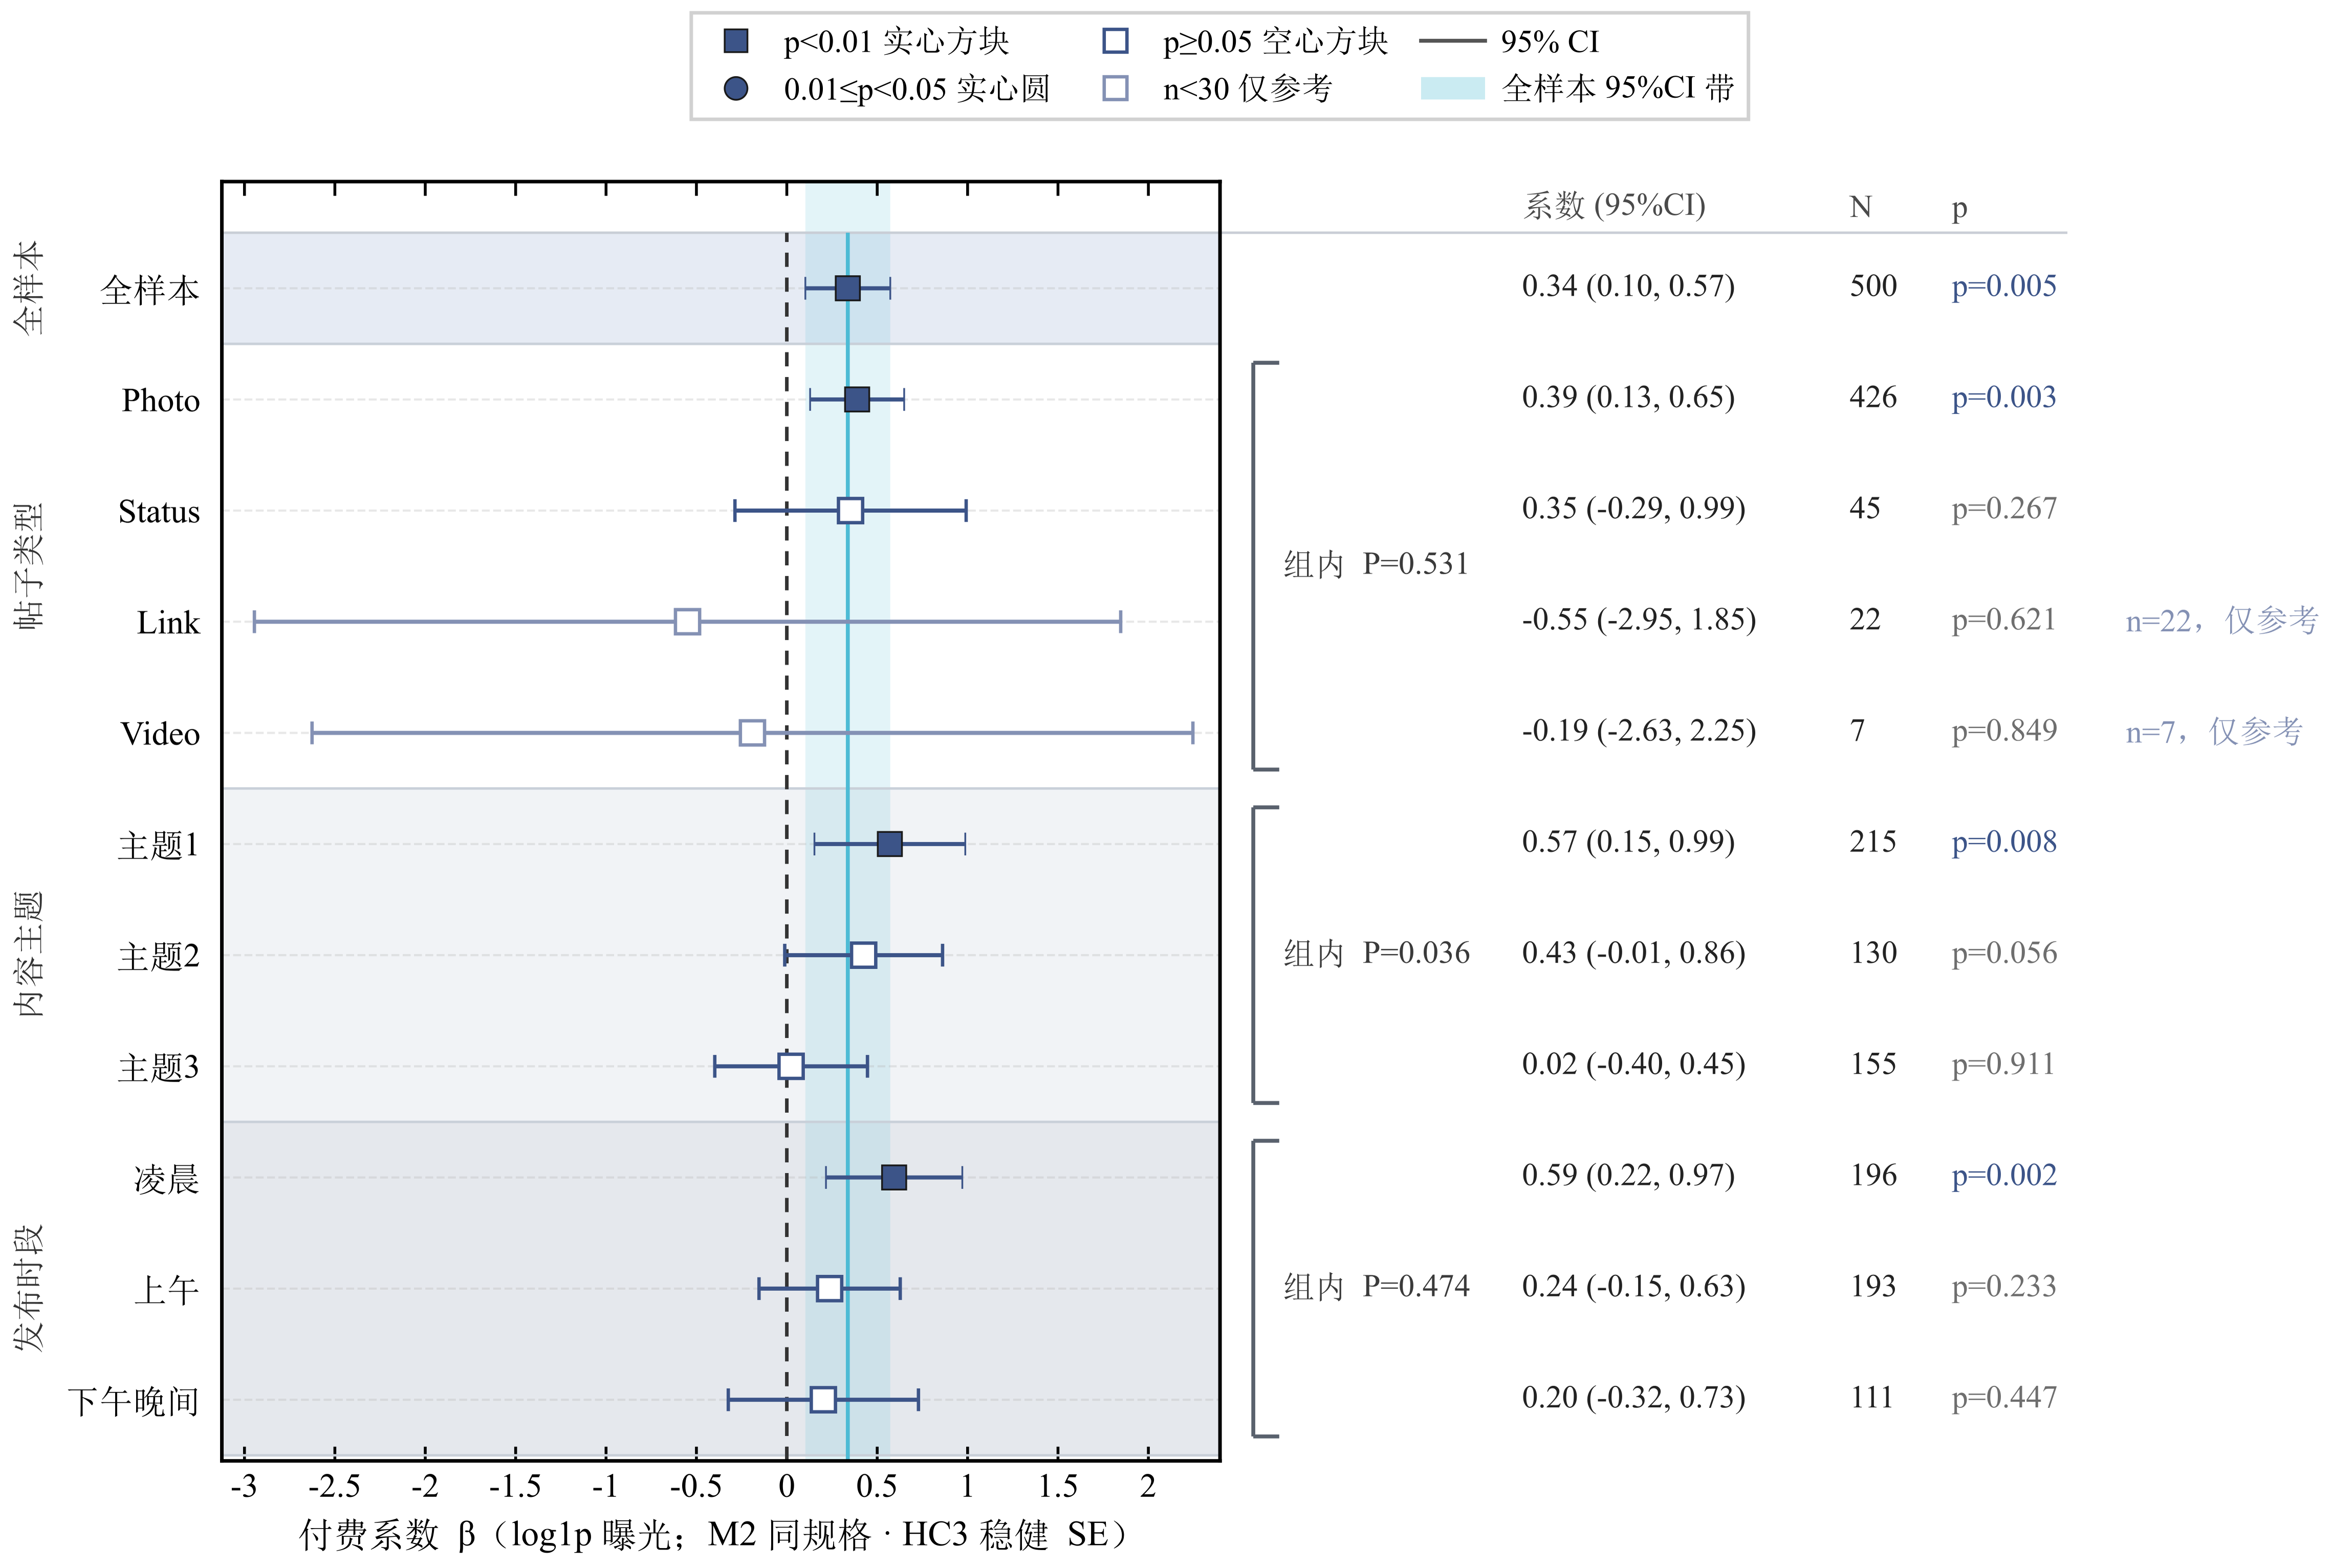
\includegraphics[width=0.70\textwidth]{../求解/问题四/结果/图17_付费效应异质性森林.png}
  \caption{付费效应在类型、主题与时段分组下的异质性}
  \label{fig:q4_het}
\end{figure}

综合以上结果，付费平均带来约 40\% 的曝光提升，代表性画像上约为 1.6 万次增量；视频相对图片约为 4.9 倍，方向明确但精度受 7 条样本限制；状态类型约为 3.2 倍，链接类型与图片无显著差异；内容主题整体显著，主题 2 与主题 3 都低于主题 1，但两者之间差异不显著。付费效应在主题维度存在异质性，主题 1 的增量最大，主题 3 接近于零。上述结论在六种模型设定下保持一致，可作为品牌主页内容编排与付费投放的参考。

